% -*- TeX -*- -*- Soft -*-

We make an explicit correspondence between the game denotation of a term and its syntax. Our approach follows ideas recently introduced in \cite{OngLics2006}, mainly the notion of computation tree of a simply-typed $\lambda$-term and traversals over the computation tree. A computation tree can be regarded as an abstract syntax tree (AST) of the $\eta$-long normal form of a term. A traversal is a justified sequence of nodes of the computation tree respecting some formation rules. Traversals are used to describe computations. An interesting property is that the \emph{P-view} of a traversal (computed in the same way as P-view of plays in Game Semantics) is a path in the computation tree.

The main result of this paper is called the \emph{Correspondence Theorem} (theorem \ref{thm:correspondence}). It states that traversals over the computation tree are just representations of the uncovering of plays in the strategy-denotation of the term. Hence there is an isomorphism between the strategy denotation of a term and its revealed game denotation ({\it i.e.}~its strategy denotation where internal moves are not hidden after composition). This theorem permits us to explore the effect that a given syntactic restriction (such as the safety restriction) has on the strategy denoting a term.

To really make use of the Correspondence Theorem, it will be necessary to restate it in the standard game-semantic framework in which internal moves are hidden. For that purpose, we will define a \emph{reduction} operation on traversals responsible of eliminating the nodes corresponding to ``internal moves'' of the game-semantics. This leads to a correspondence between the standard game denotation of a term and the set of reductions of traversals over its computation tree. Fortunately, the reduction operation preserves the good properties of traversals. This is guaranteed by the facts that the P-view of
the reduction of a traversal is equal to the reduction of the P-view of the traversal, and the O-view of a traversal is the same as the
O-view of its reduction (Proposition \ref{prop:oview_trav_projection}). \vspace{8pt} \emph{Related works}: Traversals of a computation tree provide a way to perform \emph{local computation} of $\beta$-reductions as opposed to a global approach where the $\beta$-reduction is implemented by
performing substitutions. A notion of local computation of $\beta$-reduction has been investigated in \cite{DanosRegnier-Localandasynchronou} through the use of special graphs called ``virtual nets'' that embed the lambda-calculus.

In \cite{DBLP:conf/lics/AspertiDLR94}, a notion of graph based on Lamping's graphs \citep{lamping} is introduced to represent $\lambda$-terms. The authors unify different notions of paths (regular, legal, consistent and persistent paths) that have appeared in the literature as ways to implement graph-based reduction of lambda-expressions. We can regard a traversal as an alternative notion of path adapted to the graph representation of $\lambda$-expressions given by computation trees.

%Is there any unsafe term whose game semantics is a strategy where
%pointers can be recovered?
%
%The answer is yes: take the term $T_i = (\lambda x y . y) M_i S$
%where $i =1..2$ and $\Gamma \vdash_s S : A$. $T_1$ and $T_2$ both
%$\beta$-reduce to the safe term $S$, therefore
%$\sem{T_1}=\sem{T_2}=\sem{S}$. But $T_1$ is safe whereas $T_2$ is
%unsafe. Since it is possible to recover the pointer from the game
%semantics of $S$, it is as well possible to recover the pointer from
%the semantics of $T_2$ which is unsafe.

\section{Computation tree}
We work in the general setting of the simply-typed
$\lambda$-calculus extended with a fixed set $\Sigma$ of
higher-order uninterpreted constants.\footnote{A constant $f$ is
  \emph{uninterpreted} if the small-step semantics of the language
  does not contain any rule of the form $f \dots \rightarrow e$. $f$
  can be regarded as a data constructor.}

For the rest of the section we fix a simply-typed term-in-context
$\Gamma \vdash M :T$.

\subsection{\texorpdfstring{$\eta$}{eta}-long normal form}

The $\eta$-long normal form appeared in
\citep{DBLP:journals/tcs/JensenP76} and
\citep{DBLP:journals/tcs/Huet75} under the names \emph{long reduced
form} and \emph{$\eta$-normal form} respectively. It was then
investigated in \citep{huet76} under the name \emph{extensional
form}.

The $\eta$-expansion of $M: A\typear B$ is defined as the term
$\lambda x . M x : A\typear B$ where $x:A$ is a fresh variable. Similarly, we can define the $\eta$-long-expansion of a term $M : (A_1,\ldots,A_n,o)$ as $\lambda \varphi_1 \ldots \varphi_l . M \varphi_1 \ldots \varphi_l$
where the $\varphi_i:A_i$ are fresh variables.
The \defname{$\eta$-normal
form} of a term is defined to be the term obtained by hereditarily $\eta$-long-expanding the body of every lambda abstraction as well as every subterm occurring
at an operand position (\ie occurring in the second argument of some
occurrence of the binary application operator, that is to say in $v$
for some subterm of the form $\ldots (t~v) \ldots$).
Formally:
\begin{definition}[$\eta$-long normal form]
A simply-typed term is either an abstraction or it can be written uniquely as
$s_0 s_1 \ldots s_m$ where $m\geq0$ and $s_0$ is a variable, a $\Sigma$-constant or an abstraction.

The $\eta$-long normal form of a term $t:(A_1,\ldots,A_n,o)$ for $n \geq 0$, written $\elnf{t}$ or sometimes $\etalnf{t}$, is defined by cases according to
the syntactic shape of $t$:
\begin{align*}
\elnf{\lambda x . s } &= \lambda x . \elnf{s} \\
\elnf{\alpha s_1 \ldots s_m } &= \lambda \overline{\varphi} . \alpha \elnf{s_1}\ldots \elnf{s_m} \elnf{\varphi_1} \ldots \elnf{\varphi_n}
\\
\elnf{(\lambda x . s) s_1 \ldots s_p } &= \lambda \overline{\varphi} . (\lambda x . \elnf{s}) \elnf{s_1} \ldots \elnf{s_p} \elnf{\varphi_1} \ldots \elnf{\varphi_n}
\end{align*}
where $m\geq0$, $p\geq 1$, $x$ is either a variable or a constant, $\overline{\varphi} = \varphi_1 \ldots \varphi_n$, each $\varphi_i : A_i$ is a fresh variable and $\alpha$ is either a variable or a constant.
\end{definition}

In the case $n=0$ we have
$\elnf{x s_1 \ldots s_m : o} = \lambda . x \elnf{s_1} \elnf{s_2} \ldots \elnf{s_m}$.
The `dummy' lambda in the right-hand side of the equation is deliberately kept as it plays an important role in the correspondence with game semantics.



Note that this version of the $\eta$-long normal form is defined for any simply-typed lambda term, whether $\beta$-normal or not.
Furthermore, since the transformation does not introduce any new redex, the $\eta$-long normal form of a $\beta$-normal
  term is also $\beta$-normal.




%\begin{lemma}
%The $\eta$-long normal form of a term in $\beta$-normal form is also in $\beta$-normal form.
%\end{lemma}
%\begin{proof}
%By induction on the structure of the term and the order of its type.
%\emph{Base case}:
%If $M=x:0$ then $\elnf{x} = \lambda . x$ is also in $\beta$-nf.
%\emph{Step case}:
%The case $M = (\lambda x . s) s_1 \ldots s_m : (A_1,\ldots,A_n,o)$ with $m>0$ is not possible since $M$ is in
%$\beta$-normal form.
%Suppose $M = \lambda x . s$ then $s$ is in $\beta$-nf. By the induction hypothesis $\elnf{s}$ is also in $\beta$-nf and therefore
%so is $\elnf{M} = \lambda x . \elnf{s}$.
%
%Suppose $M= \alpha s_1 \ldots s_m : (A_1,\ldots,A_n,o)$. Let $i,j$
%range over $1..n$ and $1..m$ respectively. The $s_j$ are in
%$\beta$-nf and the $\varphi_i$ are variables of order smaller than
%$M$, therefore by the induction hypothesis the $\elnf{\varphi_i}$ and
%the $\elnf{s_j}$ are in $\beta$-nf. Hence $\elnf{M}$ is also in
%$\beta$-nf.
%\end{proof}



\subsection{Computation tree}
The computation tree of a term is a certain tree representation of its
$\eta$-long normal form. It is defined as follows:

\begin{definition}
\label{dfn:comptree} Let $M$ be a simply-typed term in $\eta$-normal
form. Then $M$ must be of the form $\lambda \overline{x} . s_0 s_1
\ldots s_m$ where $s_0 s_1 \ldots s_m$ is of ground type and either
$s_0$ is a variable or a constant and $m\geq0$ or $s_0$ is an
abstraction $\lambda\overline{y}.s$ and $m\geq1$, where $s$ and the
$s_j$'s for $j\in 1..m$ are in $\eta$-normal form.

We define the tree $\tau^*(M)$ by induction on the structure of the
term as follows:
\begin{itemize}[-]
\item If $m\geq0$ and $\alpha$ is a variable or constant then:
$$ \tau^*( \lambda\overline{x} . \alpha s_1 \ldots s_m : o) =
\begin{tikzpicture}[baseline=(A.base),level distance=4ex,inner ysep=0.5mm,shape border rotate=90,sibling distance=15mm]
    \node{$\lambda\overline{x}$}
        child { node{$\alpha$}
                child[child anchor=north]{node[isosceles triangle,draw,anchor=north]{$\tau^*(s_1)$}}
                child{node{$\ldots$}}
                child[child anchor=north]{node[isosceles triangle,draw,anchor=north]{$\tau^*(s_m)$}}
        };
\end{tikzpicture}
$$

\item If $m \geq 1$ and $s_0$ is an abstraction then:
\begin{align*}
 \tau^*(\lambda\overline{x} . (\lambda\overline{y}.s) s_1 \ldots s_m : o)=
\begin{tikzpicture}[baseline=(A.base),level distance=4ex,inner ysep=0.5mm,shape border rotate=90,sibling distance=20mm]
    \node{$\lambda\overline{x}$}
        child { node{$@$}
                child[child anchor=north]{node[isosceles triangle,draw,anchor=north]{$\tau^*(\lambda\overline{y}.s)$}}
                child[child anchor=north]{node[isosceles triangle,draw,anchor=north]{$\tau^*(s_1)$}}
                child{node{$\ldots$}}
                child[child anchor=north]{node[isosceles triangle,draw,anchor=north]{$\tau^*(s_m)$}}
        };
\end{tikzpicture}
\end{align*}
\end{itemize}

Let $M$ be a simply-typed term not necessarily in $\eta$-normal
form. Let $\mathcal{D}$ denote the set of values of base type $o$.
The \defname{computation tree} of $M$, written $\tau(M)$ is the tree
obtained from $\tau^*(\etalnf{M})$ by adding leaves to the nodes as follows: every node $n \in \tau(M)$ has a
child leaf labelled $v_n$, called \defname{value-leaf}, for every
possible value $v \in \mathcal{D}$.
\end{definition}

The inner nodes of the tree are of three kinds:
\begin{itemize}
\item $\lambda$-nodes labelled $\lambda \overline{x}$ (note that a $\lambda$-node represents several consecutive variable abstractions),
\item application nodes labelled @,
\item variable or constant nodes labelled $\alpha$ for some constant or variable $\alpha$.
\end{itemize}
A node is said to be \defname{prime} if it is the 0$^{th}$ child of an @-node.
An inner node whose parent is a @-nodes or a $\Sigma$-node is called a \defname{spawn} node.
\bigskip

\begin{example}
\label{examp:comptree}
  Take $\stentail \lambda f^{o \typear o} .
(\lambda u^{o \typear o} . u) f : (o \typear o) \typear
o \typear o$.
\bigskip

\noindent
\begin{tabular}{cc}
Its $\eta$-long normal form is: & Its computation tree is:\\[8pt]
\begin{minipage}{0.45\textwidth}
\centering
$\begin{array}{ll}
 &\stentail  \lambda f^{o \typear o} z^o . \\
&\qquad(\lambda u^{o \typear o} v^o . u (\lambda.v)) \\
&\qquad(\lambda y^o. f y) \\
&\qquad(\lambda.z) \\
&: (o \typear o) \typear o \typear o
\end{array}$
\end{minipage}
&
\begin{minipage}{0.45\textwidth}
\centering
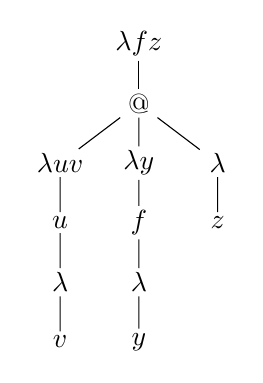
\begin{tikzpicture}[baseline=(root.base),level distance=5ex,inner ysep=0.5mm,sibling distance=10mm]
\node (root) {$\lambda f z$}
child {node {$@$}
    child {node {$\lambda u v$}
           child {node {$u$}
                  child {node {$\lambda$}
                      child {node {$v$}}
                  }
           }
    }
    child {node {$\lambda y$}
           child {node {$f$}
                  child {node {$\lambda$}
                      child {node {$y$}}
                  }
           }
    }
    child {node {$\lambda$}
           child {node {$z$}}
    }
    };
\end{tikzpicture}
\end{minipage}
\end{tabular}
\end{example}

\begin{example}
  Take $\stentail \lambda u^o v^{((o \typear o) \typear o)} . (\lambda x^o . v (\lambda z^o . x)) u : o \typear ((o \typear o) \typear o) \typear o$.
  \bigskip

\noindent
\begin{tabular}{cc}
Its $\eta$-long normal form is: & Its computation tree is:\\[8pt]
\begin{minipage}{0.45\textwidth}
\centering
$\begin{array}{ll}
 &\stentail  \lambda u^o v^{((o \typear o) \typear o)} . \\
&\qquad(\lambda x^o . v (\lambda z^o . x)) u \\
&: o \typear ((o \typear o) \typear o) \typear o
\end{array}$
\end{minipage}
&
\begin{minipage}{0.45\textwidth}
\centering
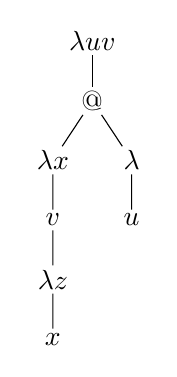
\begin{tikzpicture}[baseline=(root.base),level distance=5ex,inner ysep=0.5mm,sibling distance=10mm]
\node (root) {$\lambda u v$}
child {node {$@$}
    child {node {$\lambda x$}
           child {node {$v$}
                  child {node {$\lambda z$}
                      child {node {$x$}}
                  }
           }
    }
    child {node {$\lambda$}
           child {node {$u$}}
    }
    };
\end{tikzpicture}
\end{minipage}
\end{tabular}
\end{example}


\emph{Notations:} We write $\theroot$ to denote the root of
$\tau(M)$. We write $E$ to denote the parent-child relation of the
tree, $V$ for the set of vertices (leaves and inner nodes) of the
tree, $N$ for the set of inner nodes and $L$ for the set of
value-leaves. Thus $V = N \union L$.

We write $N_\Sigma$ for the set of $\Sigma$-labelled nodes, $N_@$ for the set
of @-labelled nodes, $N_{\sf var}$ for the set of variable nodes,
$N_{\sf fv}$ for the subset of $N_{\sf var}$ constituted of free-variable nodes, $N_{\sf prime}$ for the set of prime nodes
and $N_{\sf spawn}$ for the set of spawn nodes ($= N \inter E \relimg{N_@ \union N_\Sigma}$).

For $\$$ ranging in $\{@, \lambda, {\sf var}, {\sf fv} \}$,
we write $L_\$$ to denote the set of value-leaves of nodes from $N_\$$
{\it i.e.}\ $L_\$ = \{ v_n \ | \ n \in N_\$, v \in \mathcal{D} \}$,
and $V_\$$ to denote the set of nodes of $N_\$$ or value-leaves of nodes of $N_\$$
{\it i.e.}\ $V_\$ = N_\$ \union L_\$ $.

For any lambda node $n$ in $N_\lambda$ we write
$M^{(n)}$ for the subterm rooted at $n$ and $V^{(n)}$ for the set of nodes and leaves of the sub-computation tree $\tau(M^{(n)})$ (thus $V^{(n)} = E^*(\{n\})$).


Let $\mathcal{T}$ denote the set of $\lambda$-terms.
Each subtree of the computation tree $\tau(M)$ represents a subterm of $\elnf{M}$.
We define the function $\kappa : N \rightarrow \mathcal{T}$ that maps a node $n \in N$ to the subterm of $\elnf{M}$
corresponding to the subtree of $\tau(M)$ rooted at $n$.
In particular $\kappa(r) = \elnf{M}$.

\begin{definition}[Type and order of a node]
\label{def:nodeorder}
Suppose $\Gamma \vdash M : T$.
The \defname{type} of a node $n \in N$ of $\tau(M)$ written $\typeof{n}$ is defined as follows:
\begin{eqnarray*}
\typeof{\theroot} &=& \Gamma \typear T \\
\hbox{for $n \in (N_\lambda \union N_@) \setminus \{\theroot \}$: } \typeof{n} &=& \hbox{type of the term $\kappa(n)$,} \\
\hbox{ for $n\in N_{\sf var} \union N_\Sigma$: } \typeof{n} &=& \hbox{type of the variable labelling $n$}.
\end{eqnarray*}
The order of an inner node $n$ written $\ord{n}$ is defined to be
the order of the type of $n$. The order of a value-leaf $v \in L$ is
$0$.
\end{definition}

In particular, $\ord{@} = 0$, $\ord{\lambda \overline{\xi}} = 1+
\max_{z\in \overline{\xi}} \ord{z}$ for $\lambda \overline{\xi}\neq
r$ and if the root is $\lambda \overline{\xi}$ then $\ord{r} = 1 + \max_{z\in
\overline{\xi}\union \Gamma} \ord{z}$ with the convention $\max
\emptyset = -1$.

\begin{remark} \hfill
\begin{itemize}
\item In a computation tree, nodes at even level are $\lambda$-nodes and nodes at odd level are either application nodes,
variable or constant nodes;

\item for any ground type variable or constant $\alpha$,
\begin{tikzpicture}[baseline=(root.base),level distance=5ex,inner ysep=0.5mm,sibling distance=10mm]
\node (root) {$\lambda$}
child {node {$\alpha$} };
\end{tikzpicture};

\item for any higher-order variable or constant $\alpha : (A_1,\ldots,A_p,o)$, the computation tree $\tau(\alpha)$ has the following form:
\begin{tikzpicture}[baseline=(root.base),level distance=3ex,sibling distance=15mm]
\node (root) {$\lambda$}
child {node {$\alpha$}
    child{node {$\lambda\overline{\xi_1}$}
          child{node{$\ldots$}}}
    child{node{$\ldots$}}
    child{node {$\lambda\overline{\xi_p}$}
          child{node{$\ldots$}}}
    };
\end{tikzpicture};

\item for any tree of the form
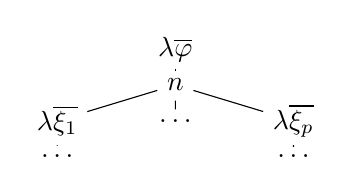
\begin{tikzpicture}[baseline=(root.base),level distance=3ex,sibling distance=15mm]
\node (root) {$\lambda\overline\varphi$}
child {node {$n$}
    child{node {$\lambda\overline{\xi_1}$}
          child{node{$\ldots$}}}
    child{node{$\ldots$}}
    child{node {$\lambda\overline{\xi_p}$}
          child{node{$\ldots$}}}
    };
\end{tikzpicture}, we have $\ord{\kappa(n)}=0$.
\end{itemize}
\end{remark}


\subsection{Pointers and justified sequence of nodes}
\subsubsection{Definitions}
\begin{definition}[Binder]
Let $n$ be a variable node of the computation tree labelled $x$. We
say that a node $n$ is bound by the node $m$, and $m$ is called the
binder of $n$, if $m$ is the closest node in the path from $n$ to
the root of the tree such that $m$ is labelled $\lambda
\overline{\xi}$ with $x\in \overline{\xi}$.
\end{definition}

\begin{definition}[Enabling]
The \defname{enabling relation} $\vdash$ is defined on the set of
nodes and leaves of the computation tree as follows. We write $m \vdash n$ and we say that $m$ enables $n$ if and only if
$m \in L \union N_\lambda \union N_{\sf var}$
and one of the following conditions holds:
\begin{itemize}
\item $n \in N_{\sf fv}$ and $m$ is the root $\theroot$;
\item $n \in N_{\sf var} \setminus N_{\sf fv}$ and
        $m$ is $n$'s binder, in which case we write $m \vdash_i n$ to precise that $n$ is the $i^{\sf th}$ variable bound by $m$;
\item $n\in N_\lambda$ and  $m$ is $n$'s parent;
\item $n \in L$ and $m$ is $n$'s parent ({\it i.e.}\ $n=v_m$ for some $v\in\mathcal{D}$).
\end{itemize}
Formally:
$$ \begin{array}{lcl}
  \vdash & = & \{ (\theroot,n) \ | n \in N_{\sf fv} \} \\
&&\union\  \{ (\lambda \overline{x},x) \ | x \in N_{\sf var}\setminus N_{\sf fv} \zand \lambda\overline{x} \mbox{ is $x$'s binder} \} \\
&& \union\ \{ (m,\lambda\overline\eta) \ | \ m \mbox{ is $\lambda\overline\eta$'s parent and } \lambda\overline\eta \in N_\lambda \} \\
&& \union\ \{ (m,v_m) \ | \ v \in \mathcal{D}, m \in N  \}
\end{array}$$
Note that in particular, free variable nodes are enabled by the root.
Table \ref{tab:enabler_type} recapitulates the possible node types for the enabler node depending on the type of $n$.
\end{definition}


\begin{table}[htbp]
$$
\begin{array}{ccl}
\mbox{If } n\in \_  & \mbox{then} & m\in \_ \\ \hline
N_\lambda & & N_{\sf var} \union N_\Sigma \union N_@ \\
L_{\sf var} & & N_{\sf var} \\
L_@ & &  N_@ \\
L_\Sigma & & N_\Sigma\\
\\
N_{\sf var} & & N_\lambda\\
N_\Sigma & & \mbox{n.a.} \\
N_@ & & \mbox{n.a.} \\
L_\lambda & & N_\lambda\\
\end{array}
$$
\caption[Category of the justifying node]{Category of the enabler node in ``$m\vdash n$''.}
\label{tab:enabler_type}
\end{table}

We say that a node $n_0$ of the computation tree is \defname{hereditarily enabled} by $n_p \in N$ if there are nodes $n_1,\ldots, n_{p-1} \in N$ such that $n_{i+1}$ enables $n_{i}$
for all $i\in 0..p-1$.

For any set of nodes $S, H \subseteq N$ we write $S^{H\vdash}$ for $S \inter \vdash^*(H) = \{ n \in S \ | \exists n_0 \in H \mbox{ s.t. }n_0  \vdash^* n \}$ -- the subset of $S$ constituted of nodes hereditarily enabled by some node in $H$. We will abbreviate $S^{\{n_0\}\vdash}$ into $S^{n_0\vdash}$.

We call \defname{input-variables nodes} the elements of $V_{\sf var}^{\theroot\vdash}$ i.e.\
variables that are hereditarily enabled by the root of $\tau(M)$. Thus we have
$V_{\sf var}^{\theroot\vdash} = V \setminus ( V_{\sf var}^{N_@\vdash}
\union V_{\sf var}^{N_\Sigma\vdash})$.
\smallskip

We use the following numbering conventions:
the first child of a @-node - a prime node - is numbered $0$;
the first child of a variable or constant node is numbered $1$;
and variables in $\overline{\xi}$ are numbered from $1$ onward ($\overline{\xi} = \xi_1 \ldots \xi_n$).
We write $n.i$ to denote the $i$th child of node $n$.

\begin{definition}[Justified sequence of nodes]
\label{dfn:justseqnode} A \defname{justified sequence of nodes} is a
sequence of nodes $s$ of the computation tree $\tau(M)$ with
pointers. Each occurrence in $s$ of a node $n$
in $L \union N_\lambda \union N_{\sf var}$ has a link pointing to some preceding occurrence of a node $m$ verifying $m \vdash n$;
and occurrences of nodes in $N_@ \union N_\Sigma$ do not have pointer.

If an occurrence $n$ points to an occurrence $m$ in $s$ then we say that $m$ \defname{justifies} $n$.
If $n$ is an inner node then we represent this pointer in the sequence as \Pstr[0.4cm]{(m){m} \ldots (n-m,45:i) n } where the label indicates that either $n$ is labelled with the $i$th variable abstracted by the
$\lambda$-node $m$ or that $n$ is the $i^{\sf th}$ child of $m$.
For leaves, pointers are represented as
$\Pstr[0.5cm]{ (m){m} \cdot \ldots \cdot (vm-m,40:v){v_m} }$.
\end{definition}

Thus a pointer in a justified sequence of nodes has
one of the following forms:
\smallskip

\begin{tabular}{clp{8cm}}
    & \Pstr[0.7cm]{ (m){r} \cdot \ldots \cdot (n-m,40){z} }
    & for some occurrences $r$ of $\tau(M)$'s root and $z \in N_{\sf fv}$;
\\
    or
    & \Pstr[0.7cm]{ (m){\lambda \overline{\xi}} \cdot \ldots \cdot (n-m,40:i){\xi_i} }
& for some variable $\xi_i$ bound by $\lambda \overline{\xi}$, $i \in 1..|\overline{\xi}|$;
\\
    or
    & \Pstr[0.7cm]{ (m){@} \cdot \ldots \cdot (n-m,40:j){\lambda \overline{\eta}} }
    & $j\in \{ 1 ..(arity(@)-1) \}$;
\\
    or
    & \Pstr[0.7cm]{ (m){\alpha } \cdot \ldots \cdot (n-m,40:k){\lambda \overline{\eta}} },
    & for $\alpha \in N_{\Sigma} \union N_{\sf var}$,  $k \in \{ 1 ..arity(\alpha) \}$;
\\
    or
    & $\Pstr[0.7cm]{ (m){m} \cdot \ldots \cdot (vm-m,40:v){v_m} }$
    & for some value $v\in \mathcal{D}$.
\end{tabular}
\bigskip


We say that an inner node $n$ in of a justified sequence of nodes is
\defname{answered}\footnote{This terminology is deliberately suggestive of the correspondence with game-semantics.} by the value-leaf $v_n$ if there is an occurrence of $v_n$ for some value $v$ in the
sequence that points to $n$, otherwise we say that $n$ is
\defname{unanswered}. The last unanswered node is called the
\defname{pending node}.  A justified sequence of nodes is
\defname{well-bracketed} if each value-leaf occurring in it is justified by the pending node at that point.

For any justified sequence of nodes and leaves $t$ we write $?(t)$
to denote the subsequence of $t$ consisting only of unanswered
nodes. Formally:
\begin{align*}
  ?(\Pstr[0.4cm]{u_1 \cdot (n){n} \cdot u_2 \cdot (nv-n){v_n} }  ) &= ?(u_1 \cdot n \cdot u_2) \setminus \{ n \}
        & \mbox{for some value $v\in\mathcal{D}$} \\
  ?(u \cdot n)   &= ?(u)\cdot n    & \mbox{for $n\not\in L$}
\end{align*}
where $u \setminus \{ n \}$ denotes the subsequence of $u$ obtained by removing the occurrence $n$.

If $u$ is a well-bracketed sequences then $?(u)$ can be defined as follows:
\begin{align*}
  ?(\Pstr[0.4cm]{u \cdot (n){n} \ldots (nv-n){v_n} }  ) &= ?(u)
          & \mbox{for some value $v\in\mathcal{D}$}  \\
    ?(u \cdot n) &= ?(u)\cdot n    & \mbox{where $n\not\in L$} \ .
\end{align*}

\bigskip

\emph{Notations}: We write $s = t$ to denote that the justified sequences $t$ and $s$
have same nodes \emph{and} pointers. Justified sequence of nodes can
be ordered using the prefix ordering: $t \sqsubseteq t'$ if and only
if $t=t'$ or the sequence of nodes $t$ is a finite prefix of $t'$
(and the pointers of $t$ are the same as the pointers of the
corresponding prefix of $t'$). Note that with this definition,
infinite justified sequences can also be compared. This ordering
gives rise to a complete partial order.
We say that a node $n_0$ of a justified sequence is \defname{hereditarily justified} by $n_p$ if there are nodes $n_1, n_2, \ldots n_{p-1}$ in the sequence such that for all $i\in 0..p-1$, $n_i$ points to $n_{i+1}$.
We write $t^\omega$ to denote the last occurrence of $t$ and $\ip(t)$ for the immediate prefix of $t$ obtained by removing $t$'s last occurrence. We write $\jp(t)$ for the sequence $t_{\prefixof j}$ where $j$ is the justifier of $t^\omega$ in $t$.
\smallskip

\subsubsection{Projection}

We define two different projection operation on justified sequences
of nodes.

Let $A$ be a subset of $V$, the set of nodes and leaves of
$\tau(M)$, and $t$ be  a justified sequence of nodes then we write
$t\filter A$ for the subsequence of $t$ consisting of nodes in $A$.
This operation can cause a node $n$ to lose its pointer. In that
case we reassign the target of the pointer to be the last node in
$t_{\prefixof n}\filter A$ that hereditarily justifies $n$ ({\it
i.e.}\ this node can be found by following the pointers from $n$
until we reach a node that appear in $A$). If there is no such node
then $n$ just loses its pointer.


\begin{definition}[Hereditary projection]
Let $t$ be a justified sequence of nodes of $\travset(M)$ and $n$ be
some occurrence in $t$. We define the justified sequence $t \filter
n$ as  the subsequence of $t$ consisting of nodes hereditarily
justified by $n$ in $t$.
\end{definition}

\begin{lemma}
\label{lem:projection_continuous} The projection function $\_
\filter n$ defined on the cpo of justified sequences ordered by the
prefix ordering is continuous.
\end{lemma}
\begin{proof}
Clearly $\_ \filter n$ is monotonous.
Suppose that $(t_i)_{i\in\omega}$ is a chain of justified sequences. Let $u$ be a finite prefix of $(\bigvee t_i) \filter n$.
Then $u = s \filter n$ for some finite prefix $s$ of $\bigvee t_i$. Since $s$ is finite we must have $s \prefixof t_j$ for some $j\in\omega$.
Therefore $u \prefixof t_j \filter n \prefixof \bigvee (t_j \filter  n)$.
This is valid for any finite prefix $u$ of $(\bigvee t_i) \filter n$ thus $(\bigvee t_i) \filter  n \prefixof \bigvee (t_j \filter n)$.
\end{proof}


The nodes occurrences that do not have pointers in a justified
sequence are called \defname{initial occurrences}. An initial
occurrence is either the root of the computation tree,
an @-node or a $\Sigma$-node. Let $n$ be occurrence in a justified
sequence of nodes $t$. We call
\defname{thread of the occurrence $n$} the subsequence of $t$
consisting of occurrences that are her.\ just.\ by the same initial
occurrence. In other words the thread of $n$ is $n \filter i$ where
$i$ is the first node in $t$ hereditarily justifying $n$; $i$ is
called the \defname{initial occurrence of the thread of $n$}.

\subsubsection{Views}
The notion of \defname{P-view} $\pview{t}$ of a justified sequence
of nodes $t$ is defined the same way as the P-view of a justified
sequences of moves in Game Semantics:

\begin{definition}[P-view of justified sequence of nodes]
The P-view of a justified sequence of nodes $t$ of $\tau(M)$, written $\pview{t}$, is defined as follows:
$$\begin{array}{rcll}
 \pview{\epsilon} &=&  \epsilon \\
 \pview{s \cdot n }  &=&  \pview{s} \cdot n
    & \mbox{for $n \in N_{\sf var} \union N_\Sigma \union N_@ \union L_\lambda$;}
    \\
 \pview{\Pstr[10pt]{ s \cdot (m){m} \cdot \ldots \cdot (lmd-m,25){n}}} &=&
        \Pstr{ \pview{s} \cdot (m2){m} \cdot (lmd2-m2,60){n} }
    & \mbox{for $n \in L_{\sf var} \union L_\Sigma \union L_@ \union N_\lambda$;}
    \\
 \pview{s \cdot r }  &=&  r
    & \mbox{if $r$ is an occurrence of $\theroot$, the root of the tree $\tau(M)$. }
\end{array}$$
The equalities in the definition determine pointers implicitly. For
instance in the second clause, if in the left-hand side, $n$ points
to some node in $s$  that is also present in $\pview{s}$ then in the
right-hand side, $n$ points to that occurrence of the node in
$\pview{s}$.
\end{definition}

The O-view of $s$, written $\oview{s}$, is defined dually.
\begin{definition}[O-view of justified sequence of nodes]
\label{dfn:oview} The O-view of a justified sequence of nodes $t$ of
$\tau(M)$, written $\oview{t}$, is defined as follows:
$$\begin{array}{rcll}
 \oview{\epsilon} &=&  \epsilon \\
 \oview{s \cdot n }  &=&  \oview{s} \cdot n
    & \mbox{for $n \in L_{\sf var} \union L_\Sigma \union L_@ \union N_\lambda$;}
    \\
 \oview{\Pstr[10pt]{s \cdot (m){m} \cdot \ldots \cdot (x-m,30){n}}} &=&
    \Pstr{ \oview{s} \cdot (m2){m} \cdot (n2-m2,60){n} }
    & \mbox{for $n \in N_{\sf var} \union L_\lambda$;}
%    (if $n \in N_{\sf var}$ then the pointer considered is its main link);}
    \\
 \oview{s \cdot n }  &=&  n
    & \mbox{for $n \in N_@ \union N_\Sigma$.}
\end{array}$$
\end{definition}

We borrow some game semantic terminology:
\begin{definition} A justified sequence of nodes $s$ satisfies:
\begin{itemize}[-]
\item \defname{Alternation} if for any two consecutive nodes in $s$, one is in $V_\lambda$ and not the other one;
\item \defname{P-visibility} if for every occurrence in $s$
of a node in $N_{\sf var} \union L_\lambda$, its justifier occur in the P-view a that point;
\item  \defname{O-visibility} if the justifier of each lambda node in $s$ occurs in the O-view a that point.
\end{itemize}
\end{definition}

\begin{property}
\label{proper:pview_visibility}
The P-view (resp. O-view) of a justified sequence verifying P-visibility (resp. O-visibility)
is a well-formed justified sequence verifying P-visibility (resp. P-visibility).
\end{property}
This is proved by an easy induction.


\subsection{Traversal of the computation tree}
\label{subsec:traversal}
A \emph{traversal} is a justified sequence of nodes of the computation tree where each node indicates a step that is taken during the evaluation of the term.

\subsubsection{Traversals for simply-typed \texorpdfstring{$\lambda$}{lambda}-terms}

We first consider the simply-typed $\lambda$-calculus without interpreted constants.
Everything remains valid in the presence of \emph{uninterpreted} constants as we can just
consider them as free variables.

We define the notion of traversal over the computation tree $\tau(M)$.
We will then we show how to extend the notion of traversal to more general settings with interpreted constants.

\begin{definition}[Traversals for simply-typed $\lambda$-terms] \rm
\label{def:traversal} The set $\travset(M)$ of \defname{traversals}
over $\tau(M)$ is defined by induction over the rules of Table
\ref{tab:trav_rules}. A traversal that cannot be extended by any
rule is said to be \emph{maximal}.
\end{definition}

\begin{FramedTable}
\noindent {\bf Initialization rules}
\begin{itemize}[]
\item\rulenamet{Empty} $\epsilon \in \travset(M)$.
\item\rulenamet{Root} The sequence constituted of a single occurrence of $\tau(M)$'s root is a traversal.
\end{itemize}

\noindent {\bf Structural rules}
\begin{itemize}[]
    \item \rulenamet{Lam} If $t \cdot \lambda \overline{\xi}$ is a traversal then so is
        $t \cdot \lambda \overline{\xi} \cdot n$ where $n$
        denotes $\lambda \overline{\xi}$'s child and:
        \begin{compactitem}
            \item If $n \in N_@ \union N_\Sigma$ then it has no justifier;
            \item if  $n \in N_{\sf var}\setminus N_{\sf fv}$ then it points to the only occurrence\footnote{Prop.\ \ref{prop:pviewtrav_is_path} will show that P-views
            are paths in the tree thus $n$'s enabler occurs
            exactly once in the P-view.} of its binder in
            $\pview{t\cdot \lambda \overline{\xi}}$;
            \item if  $n \in N_{\sf fv}$ then it points
            to the only occurrence of the root $\theroot$ in
            $\pview{t \cdot \lambda \overline{\xi}}$.
        \end{compactitem}
    \item \rulenamet{App} If $t \cdot @$ is a traversal then so is \Pstr[0.4cm]{t \cdot (m) @  \cdot (n-m,40:0) n}.
\end{itemize}

\emph{\bf Input-variable rules}
\begin{itemize}[]
\item \rulenamet{InputVar} If $t$ is a traversal where $t^\omega \in N_{\sf var}^{\theroot\vdash} \union L_\lambda^{\theroot\vdash}$
and $x$ is an occurrence of a variable node in $\oview{t}$ then
so is $t \cdot n$ for any child $\lambda$-node $n$ of $x$, $n$
pointing to $x$.



\item \rulenamet{InputValue} If $t_1
\cdot x \cdot t_2$ is a traversal with pending node $x \in
N_{\sf var}^{\theroot\vdash}$ then so is \Pstr[0.5cm]{t_1 \cdot
(x){x} \cdot t_2 \cdot (xv-x,38:v){v_x} } for all $v \in
\mathcal{D}$.
\end{itemize}

\emph{\bf Copy-cat rules}
\begin{itemize}[]
\item\rulenamet{Var}
If \Pstr[0.5cm]{t \cdot (n){n} \cdot (lx){\lambda \overline{x}}
    \ldots (x-lx,50:i){x_i} } is a traversal where $x_i \in
    N_{\sf var}^{@\vdash}$ then so is \Pstr[0.5cm]{ t \cdot
(n){n} \cdot (lx){\lambda \overline{x}}  \ldots (x-lx,30:i){x_i}
    \cdot (letai-n,40:i){\lambda \overline{\eta_i}}
     }.

\item\rulenamet{Value}
  If \Pstr{t \cdot (m){m} \cdot (n){n}  \ldots
(vn-n,60:v){v}_{n} } is a traversal where $n\in N$ then so is
\Pstr[0.6cm]{t \cdot (m){m} \cdot (n){n} \ldots
(vn-n,60:v){v}_{n} \cdot (vm-m,45:v){v}_m}.
\end{itemize}
\caption[Traversal rules for the simply-typed
lambda-calculus]{Traversal rules for the simply-typed
$\lambda$-calculus.}
 \label{tab:trav_rules}
\end{FramedTable}



\begin{example}
\label{examp:trav} The following justified sequence is a traversal
of the computation tree of example \ref{examp:comptree}:
$$\pstr[1.3cm]{\nd t= (n0){\lambda f z}
        \nd\cdot (n1){@}
        \nd\cdot (n2-n1){\lambda u v}
        \nd\cdot (n3-n2){u}
        \nd\cdot (n4-n1){\lambda y}
        \nd\cdot (n5-n0){f}
        \nd\cdot (n6-n5){\lambda }
        \nd\cdot (n7-n4){y}
        \nd\cdot (n8-n3){\lambda }
        \nd\cdot (n9-n2){v}
        \nd\cdot (n10-n1){\lambda }
        \nd\cdot (n11-n0){z} \ .
}$$
\end{example}


\begin{remark} \hfill
\label{rem:traversal_rules}
\begin{enumerate}
\item
    The rule \rulenamet{Value} from Table \ref{tab:trav_rules}
    can be equivalently reformulated into four distinct rules
    \rulenamet{Value^{\lambda\mapsto @}},
    \rulenamet{Value^{@\mapsto\lambda}},
    \rulenamet{Value^{\lambda\mapsto{\sf var}}} and
    \rulenamet{Value^{{\sf var}\mapsto\lambda}}, each one
    dealing with a different possible category for the nodes $n$
    and $m$:
    \begin{description}
    \item[\rulenamet{Value^{\lambda\mapsto @}}]
      If \Pstr{t \cdot (app){@} \cdot (lz-app,60:0){\lambda
    \overline{z}}  \ldots  (lzv-lz,60:v){v}_{\lambda \overline{z}} }
    is a traversal then so is \Pstr[0.5cm]{t \cdot (app){@} \cdot
    (lz-app,60){\lambda \overline{z}} \ldots
    (lzv-lz,60:v){v}_{\lambda \overline{z}} \cdot
    (appv-app,45:v){v}_@}.

    \item[\rulenamet{Value^{@\mapsto\lambda}}] If \Pstr[0.4cm]{t \cdot \lambda \overline{\xi} \cdot (x){@}  \ldots   (xv-x,50:v){v}_@}
    is a traversal then so is \Pstr[0.5cm]{t \cdot (lmd){\lambda
    \overline{\xi}} \cdot (x){@}  \ldots  (xv-x,50:v){v}_@  \cdot
    (lmdv-lmd,33:v){v}_{\lambda \overline{\xi}} }.

    \item[\rulenamet{Value^{\lambda\mapsto{\sf var}}}] If \Pstr[0.4cm]{t \cdot y \cdot (lmd){\lambda \overline{\xi}}
    \ldots (lmdv-lmd,50:v){v}_{\lambda \overline{\xi}} } is a
    traversal where $y\in N_{\sf var}^{@\vdash}$ then so is
    \Pstr[0.5cm]{t \cdot (y){y} \cdot (lmd){\lambda \overline{\xi}}
    \ldots (lmdv-lmd,30:v){v}_{\lambda \overline{\xi}}  \cdot
    (vy-y,50:v){v}_y }.

    \item[\rulenamet{Value^{var\mapsto\lambda}}] If \Pstr[0.4cm]{t \cdot \lambda \overline{\xi} \cdot (x){x}  \ldots   (xv-x,50:v){v}_x}
    is a traversal where $x\in N_{\sf var}$ then so is
    \Pstr[0.5cm]{t \cdot (lmd){\lambda \overline{\xi}} \cdot (x){x}
    \ldots  (xv-x,50:v){v}_x  \cdot (lmdv-lmd,30:v){v}_{\lambda
    \overline{\xi}} }.
    \end{description}
    In the rest of this chapter we will prove various resulting
    by induction on the structure of some traversal and by case
    analysis on the last rule used to form it. For the sake of
    these proofs, we will use the above-defined reformulation of
    \rulenamet{Value} in place of its original definition.

    \item In the rule \rulenamet{InputValue}, although it is not specified, the last node in the traversal $t_1 \cdot x \cdot t_2$ must necessarily belong to $N_{\sf var} \union L_\lambda$. Indeed, since the pending node $x$ is a variable node, it is of the form
$$\Pstr[0.5cm]{\ldots \cdot x \cdot  (l){\lambda \overline{\eta}_1}\ldots (v-l){v^1_{\lambda \overline{\eta}_1}}
(l2){\lambda \overline{\eta}_2}\ldots (v2-l2){v^2_{\lambda \overline{\eta}_2}}
\ldots (lk){\lambda \overline{\eta}_k}\ldots (vk-lk){v^k_{\lambda \overline{\eta}_k}}
}$$ for some nodes $\lambda \overline{\eta}_k$, values $v^k \in \mathcal{D}$ and $k\geq 0$; thus the last occurrence belongs to $N_{\sf var}$ if $k=0$ and to $L_\lambda$ if $k\geq1$.

    Furthermore, the pending node appears necessarily in the O-view.

    These two observations show that the rule \rulenamet{InputValue} is essentially \rulenamet{InputVar} specialized for value-leaves. The only difference is that \rulenamet{InputVar}
    allows the visited node to be justified by \emph{any} variable node occurring in the O-view whereas \rulenamet{InputValue} constrains the node
    to be justified by the pending node (which necessarily occurs in the O-view). This restriction is here to ensure that traversals are well-bracketed.

\item In the rule
\rulenamet{Value}, it is possible to replace the condition ``$n\in N$'' by the stronger ``$n\in N\setminus N_{\sf \lambda}^{\vdash\theroot}$''. Indeed a later result (Lemma \ref{lem:trav_oview_single_threaded}) will show that if $n$ belongs to $N_{\lambda}^{\vdash\theroot}$ then the preceding occurrence $m$ is necessarily an input-variable.
Furthermore, another result (Prop.\ \ref{prop:pviewtrav_is_path}) shows that traversals are well-bracketed, therefore $m$ is necessarily the pending node. Hence the rule \rulenamet{InputValue} can be use in place of
\rulenamet{Value} to visit $v_m$.


The advantage of this alternative formulation is that the traversal rules have a disjoint domains of definition.
\end{enumerate}
\end{remark}
\bigskip

A traversal always starts with the root node and mainly follows the
structure of the tree. The exception is the \rulenamet{Var} rule
which permits the traversal to jump across the computation tree. The
idea is that after visiting a non-input variable node $x$, a jump
can be made to the node corresponding to the subterm that would be
substituted for $x$ if all the $\beta$-redexes occurring in the term
were to be reduced. Let $\lambda \overline{x}$ be $x$'s binder and
suppose $x$ is the $i$th variable in $\overline{x}$. The binding
node necessarily occurs previously in the traversal (this will be
proved in Prop.\ \ref{prop:pviewtrav_is_path}). Since $x$ is not
hereditarily justified by the root, $\lambda \overline{x}$ is not
the root of the tree and therefore it is not the first node of the
traversal. We do a case analysis on the node preceding $\lambda
\overline{x}$:
    \begin{itemize}
    \item If it is an @-node then $\lambda \overline{x}$ is necessarily the first child node of that node
    and it has has exactly $|\overline{x}|$ siblings:
\begin{center}
\begin{tikzpicture}[baseline=(root.base),level distance=6ex,sibling distance=17mm,
level 2/.style={level distance=10ex},
level 3/.style={level distance=6ex}]
\node(root){}
child[dotted]{
    node[anchor=south]{$@$}
    child[solid] {node {$\lambda\overline x$}
        child[dotted,level distance=8ex]{node{$x$}}
        edge from parent node[fill=white]{$0$}
        }
    child[solid] {node {$\lambda\overline\eta_1$}
        child[dotted] {node{}}
        edge from parent node[fill=white]{$1$}
        }
    child[dotted]{node{}}
    child[solid] {node {$\lambda\overline\eta_i$}
        child[dotted]{node{}}
        edge from parent node[fill=white]{$i$}
        }
    child[dotted]{node{}}
    child[solid] {node {$\lambda\overline\eta_{|x|}$}
        child[dotted]{node{}}
        edge from parent node[fill=white]{$|x|$}
        }
};
\end{tikzpicture}
\end{center}

    In that case, the next step of the traversal is a jump to $\lambda \overline{\eta_i}$ -- the $i$th child of
    @ -- which corresponds to the subterm that would be substituted for $x$ if the $\beta$-reduction was
    performed:
    $$\Pstr[19pt]{ t' \cdot
            (n){@} \cdot
            (lx){\lambda \overline{x}} \cdot \ldots \cdot
            (x-lx,40:i){x} \cdot
            (mi-n,40:i){\lambda \overline{\eta_i}} \cdot \ldots
            \in {\travset(M)}   }
    $$

    \item If it is a variable node $y$, then
    the node $\lambda \overline{x}$ was necessarily added to the traversal $t_{\leq y}$ using the \rulenamet{Var} rule.
    (Indeed, if it was visited using \rulenamet{InputVar} then $\lambda \overline{x}$ would be hereditarily justified by the root. But this is not possible since $x_i$, bound by $\lambda \overline{x}$, is not an input-variable.)
    Therefore $y$ is substituted by the term $\kappa(\lambda \overline{x})$ during the evaluation of the term.

    Consequently, during reduction, the variable $x$ will be substituted by the subterm represented by
    the $i$th child node of $y$. Hence the following justified sequence is also a traversal:
    $$\Pstr[18pt]{ t' \cdot
            (y){y} \cdot
            (lx){\lambda \overline{x}} \cdot \ldots \cdot
            (x-lx,40:i){x} \cdot
            (mi-y,40:i){\lambda \overline{\eta_i}} \cdot \ldots
    }
    $$
    \end{itemize}

\begin{remark}
Our notions of computation tree and traversal differ slightly from \cite{OngLics2006}:
\begin{itemize}[-]
    \item In \cite{OngLics2006} computation trees can have (uninterpreted first-order) constants. At the moment we do not have taken constants into account but as we have already observed, uninterpreted constants can be just regarded as free variables, thus we do not lose any expressivity here.

    \item In \cite{OngLics2006}, constants are restricted to order one at most since computation tree
    are used to model computation of tree structures. Here we do not need this restriction (as long as constants are uninterpreted we can regard them as free variables for any higher order).


    \item In \cite{OngLics2006}, the rule \rulenamet{Sig} suffices to model the first-order constants used as constructors for tree structures. In our setting, however, we have to deal with the full power of \emph{free variables}.
        In order to model them, it was necessary to introduce the more subtle rules \rulenamet{InputValue}, \rulenamet{InputVar}.

    \item In our setting, we have introduced the notion of value-leaves. This extra machinery will be necessary when we extend traversal rules to model interpreted constants. (We will show how to do so for the constants of \pcf\ and \ialgol.)
    \end{itemize}
\end{remark}

\begin{example}
Consider the following computation tree:
\begin{center}
\begin{tikzpicture}[baseline=(root.base),level distance=5ex,inner ysep=0.5mm,sibling distance=12mm,
level 2/.style={sibling distance=40mm,level distance=5ex},
level 3/.style={sibling distance=10mm,level distance=7ex},
level 4/.style={sibling distance=10mm,level distance=6ex}]
\node (root) {$\lambda$}
child {
    node {$@$}
    child {
        node {$\lambda y$}
        child[dotted] {node {$y$}
           child{node {$\lambda\overline\eta_1$}
               child{node{}}
               edge from parent node[fill=white] {$1$}
           }
           child{node{}}
           child{node{$\lambda\overline\eta_i$}
             child{node{}}
             edge from parent node[fill=white] {$i$}
           }
           child{node{}}
           child{node{$\lambda\overline\eta_n$}
             child{node{}}
             edge from parent node[fill=white] {$n$}
           }
        }
        edge from parent node[fill=white] {$0$}
    }
    child {node{$\lambda\overline{x}$}
        child[dotted] {node{$x_i$}
           child{node{}}
           child{node{}}
        }
        edge from parent node[fill=white]{$1$}
    }
};
\end{tikzpicture}
\end{center}
An example of traversal of this tree is:
\vspace{0.3cm}
$$ \Pstr{ \lambda \cdot
            (app){@}  \cdot
            (ly){\lambda y} \cdot \ldots \cdot
            (y-ly,40:1){y} \cdot
            (lx-app,50:1){\lambda \overline{x}} \cdot \ldots \cdot
            (x-lx,40:i){x_i} \cdot
            (leta-y,50:i){\lambda \overline{\eta_i} } \cdot \ldots
        }$$
\end{example}



\begin{lemma}
\label{lem:jump_in_thread}
Take a traversal $t$ ending with an inner node hereditarily justified by an application node @. Then if we represent only the nodes appearing in the O-view, the thread of $t^\omega$ has the following shape:
$$ \Pstr[0.5cm]{ (app){@}\cdot
(l0-app){\lambda \overline{\xi}_0} \ldots (x1-l0){x_1} \cdot
(l1-app){\lambda \overline{\xi}_1} \ldots (x2-l1){x_2} \cdot
(l2-x1){\lambda \overline{\xi}_2} \ldots (x3-l2){x_3} \cdot
(l3-x2){\lambda \overline{\xi}_3} \ldots (x4-l3){x_4} \ldots
(xkm1){x_{k-1}}
(lkm1){\lambda \overline{\xi}_{k-1}} \ldots (xk-lkm1){x_k}
(lk-xkm1){\lambda \overline{\xi}_k}
 } $$
Suppose that the initial node $@$ occurs in the computation as follows:
\begin{center}
\begin{tikzpicture}[baseline=(root.base),level distance=6ex,inner ysep=0.5mm,sibling distance=15mm]
\node (root) {$\ldots$}
child {node {$@$}
    child{node {$\lambda\overline\eta_1$}
          child[dotted]{node{}}}
    child{node{$\ldots$}}
    child{node {$\lambda\overline\eta_q$}
          child[dotted]{node{}}}};
\end{tikzpicture}
\end{center}
Let us write $\tau_i$ for the sub-tree rooted at $\lambda \overline{\eta}_i$ for $i\in \{1.. q\}$.
Then for every $j\in \{1.. k\}$, $x_j$ and $\lambda \overline{\xi}_j$ must belong to two different subtrees $\tau_i$ and $\tau_{i'}$. Furthermore, $x_j$ is hereditarily justified by
some occurrence of $\lambda \overline{\eta}_i$ in $t$ and
$\lambda \overline{\xi}_j$ is hereditarily justified by
some occurrence of $\lambda \overline{\eta}_{i'}$ in $t$
(and therefore $\lambda \overline{\xi}_j \in V^{\lambda \overline{\eta}_{i} \vdash}$
and $x_j \in V^{\lambda \overline{\eta}_{i'} \vdash}$).
\end{lemma}
\proof The proof is by an easy induction. \qed


\subsubsection{Traversal rules for interpreted constants}

The framework that we have established up to know aims at providing
a computation model of simply-typed lambda terms. It is however
possible to extend it to other higher-order languages that are based
on the simply-typed lambda calculus. To achieve, one needs to
complete the core traversal rules from Table \ref{tab:trav_rules}
with new rules describing the behaviour of the interpreted constants
of the language considered. For instance in the case of \pcf, we
need to define rules for the interpreted constant $\pcfcond$ that
replicate the behaviour of the conditional operation. (In a
forthcoming section of this chapter we will give a complete
definition of the constant traversal rules for \pcf\ and \ialgol.)

We mentioned before that uninterpreted constants can be regarded as
free variables. In the same way, we can consider interpreted
constants as a \emph{generalization} of free variables: for both of
them, the ``code'' describing their computational behaviour is not
defined within the scope of the term; it is instead assumed that the
environment knows how to interpret them. Free variables, however,
have less power than interpreted constants in that when evaluating
an applicative term with a free variable in head position, the
evaluation of the head variable does not depend on the result of the
evaluation of its parameter; whereas for applicative term with an
interpreted constant in head position, the evaluation can be driven
by the result of the the evaluation of its parameter. (e.g.\ the
\pcf\ constant $\pcfcond$ is capable of branching between two of its
parameters depending on the result of the evaluation of its first
parameter.)

Based on these observation, we can define a prototype for constant
traversal rules inspired by the definition of the rules
\rulenamet{InputValue} and \rulenamet{InputVar}:
\begin{definition}[Constant traversal rule]
    \label{def:constant_traversal} A \defname{constant traversal} has
    one of the following two forms:
        $$\rulename{\Sigma\mbox{-Value}}\ \rulef{t = t_1\cdot \alpha \cdot t_2 \in \travset(M) \quad \alpha \in N_\Sigma \union N^{N_\Sigma\vdash}_{\sf var} \quad ?(t)^\omega = \alpha \quad P(t)}
          {
            \stackrel{\rule{0pt}{3pt} }{
                \Pstr[8pt]{ t' = t_1\cdot (alpha){\alpha} \cdot t_2 \cdot (v-alpha,35){v(t)} \in {\travset(M)}}
                }
           }
           $$
    or
    $$\rulename{\Sigma}/\rulename{\Sigma\mbox{-Var}}\ \rulef{t \in \travset(M) \quad t^\omega\in N_\Sigma \union N^{N_\Sigma\vdash}\union L_\lambda \quad P(t)}
      { \stackrel{  \rule{0pt}{3pt} }{\Pstr[5pt]{ t \cdot {n(t)} \in {\travset(M)}}}
       }$$
        where:
        \begin{compactitem}
          \item $P(t)$ is a predicate expressing some condition on $t$;
          \item $v(t)$ is a value-leaf of the node $\alpha$ that is determined by the traversal $t$;
          \item $n(t)$ is a lambda-node determined by $t$, and its link, also determined by $t$, points to some occurrence of its parent node in $\oview{t}$.
        \end{compactitem}
    Clearly, such rules preserve well-bracketing, alternation and visibility.
\end{definition}

\begin{remark}
The extra power of the constant rules over the input-variable rules
\rulenamet{InputValue} and \rulenamet{InputVar} lies in their
ability to base their choice of the next node to visit on
the shape of the traversal $t$.
\end{remark}

From now on, to make our argument as general as possible, we
consider a simply-typed $\lambda$-calculus language extended with
higher-order interpreted constants for which some constant traversal
rules have been defined (in the sense of Def.
\ref{def:constant_traversal}). Furthermore, we complete the set of
rules with the following additional copy-cat rule:
\begin{quote}
\rulenamet{Value^{\Sigma\mapsto\lambda}} If \Pstr[0.4cm]{t \cdot
\lambda \overline{\xi} \cdot (x){c}  \ldots   (xv-x,50:v){v}_c} is a
traversal where $c\in\Sigma$ then so is \Pstr[0.5cm]{t \cdot
(lmd){\lambda \overline{\xi}} \cdot (x){c}  \ldots  (xv-x,50:v){v}_c
\cdot (lmdv-lmd,33:v){v}_{\lambda \overline{\xi}} }.
\end{quote}


We now introduce a special kind of constant traversal rules:
\begin{definition}[Well-behaved traversal rule]
\label{def:wellbehaved_traversal} A constant traversal rules is
    \defname{well-behaved} if
    for every traversal  \Pstr[0.5cm]{ t \cdot (a){\alpha} \cdot u \cdot (n-a,35){n}} formed with the rule
    we have $?(u) = \epsilon$.
\end{definition}

The rule $\rulename{\Sigma\mbox{-Value}}$, for instance, is clearly
well-behaved (because of well-bracketing of traversals), whereas
$\rulename{\Sigma}/\rulename{\Sigma\mbox{-Var}}$ is not well-behaved
in general since $n(t)$ does not necessarily points to the pending
node in $t$.

\begin{lemma}
\label{lem:sigma_order1_are_wellbehaved} If $\Sigma$-constants have
order $1$ at most, then constant rules are necessarily all
well-behaved.
\end{lemma}
\proof In the computation tree, an order-$1$ constant hereditarily
enables only its immediate children (which are all dummy lambda
nodes $\lambda$). Hence a traversal formed with the rule
$\rulename{\Sigma}/\rulename{\Sigma\mbox{-Var}}$ is of the form:
$$\Pstr[0.5cm]{ t = \ldots \cdot (a){\alpha} \cdot u \cdot
 (n-a,35){\lambda}}$$
where $\alpha$ appears in $\oview{t}$.

If $u=\epsilon$  then the result trivially holds. Otherwise, $u$'s
first node has necessarily been visited with the rule
$\rulename{\Sigma}/\rulename{\Sigma\mbox{-Var}}$ thus $u$'s first
node is a dummy lambda node $\lambda'$ pointing to $\alpha$. Since
$\alpha$ occurs in $\oview{t}$ and since the node $\lambda'$ enables
only its value-leaf in the computation tree, $t$ must be of the
following shape:
$$\pstr[0.5cm]{ t = \ldots \cdot \nd(a){\alpha} \cdot \underbrace{\nd(lp-a,35){\lambda'} \cdot  \ldots \cdot \nd(v-lp){v_{\lambda'}} \ldots }_{u} \cdot
 \nd(l-a,35){\lambda}}$$
for some value leaf $v_{\lambda'}$ of $\lambda'$.

Again, the node following $v_{\lambda'}$ must be a dummy lambda node
pointing to $\alpha$. By iterating the same argument we obtain that
the segment $u$ is a repetition of segments of the form
\Pstr[0.5cm]{(lp){\lambda'} \cdot  \ldots (v-lp){v_{\lambda'}}}.
Hence $?(u)=\epsilon$. \qed
%%% end of proof



\subsubsection{Property of traversals}

\begin{proposition}[counterpart of proposition 6 from \cite{OngHoMchecking2006}]
\label{prop:pviewtrav_is_path}
Let $t$ be a traversal. Then:
\begin{itemize}
\item[(i)] $t$ is a well-defined and well-bracketed justified sequence;
\item[(ii)] $t$ is a well-defined justified sequence verifying alternation, P-visibility and O-visibility;
\item[(iii)] If $t^\omega \not\in L_\lambda$ {\it i.e.}~$t$'s last occurrence is not a lambda value-leaf, then $\pview{t}$ is the path in the computation tree going from the root to the node $t^\omega$.
\end{itemize}
\end{proposition}

This is the counterpart of proposition 6 from
\cite{OngHoMchecking2006} which is proved by induction on the
traversal rules. This proof can be easily adapted to take into
account the constant rules and the presence of value-leaves in the
traversal.
\begin{proof}
The proof of (i), (ii) and (iii) is done simultaneously by induction on the traversal rules. We consider the rule \rulenamet{Lam} only:
We need to show that $n$'s binder occurs only once in the P-view at that point. By the induction hypothesis (iii) we have that $\pview{t \cdot \lambda \overline{\xi}}$ is a path in the computation tree from the root to $\lambda \overline{\xi}$. But $n$'s binder occurs only once in this path, therefore the traversal $t \cdot \lambda \overline{\xi} \cdot n$ is well-defined and satisfies P-visibility. Thus (i) and (ii) are verified. Furthermore $n$ is a child of $\lambda \overline{\xi}$ therefore (iii) also holds.
\end{proof}

%In particular to prove that the copy-cat rules are well-defined, one needs to ensure that
%if the last two unanswered nodes are $y$ and $\lambda \overline{\xi}$ in that order, for some non input-variable node $y$ then necessary
%      $y$ and $\lambda \overline{\xi}$ are consecutive nodes in the traversal.
%    This is because in a traversal, a non input-variable $y$ is always followed by a lambda node and whenever this lambda node is answered
%    there is only one way to extend the traversal : by using the copy cat rule to answer the $y$ node.


\begin{lemma}
\label{lem:trav_last_not_leaf} If $t \cdot n $ is a traversal with
$n \in N_{\sf var} \union N_\Sigma \union N_@$ then $t^\omega$ is a
lambda node and is $n$'s parent in $\tau(M)$. (Thus $t^\omega$ is
not a leaf: $n\not\in L$).
\end{lemma}
\begin{proof}
By inspecting the traversal rules, we observe that \rulenamet{Lam}
is the only rule  which can visit a node in $N_{\sf var} \union
N_\Sigma \union N_@$. Hence $t'^\omega$ must be $n$'s parent in
$\tau(M)$.
\end{proof}


\begin{lemma}
\label{lem:betanorm_enabling}
Suppose that $M$ is $\beta$-normal and let $t$ be a traversal of $\tau(M)$.
For any node $n$ occurring in $t$ we have:
$$ n \not\in N^{\theroot\vdash} \quad \iff \quad n \in N^{N_{\Sigma}\vdash}$$
{\it i.e.}~ $\theroot$ does not hereditarily enable $n$ if and only if $n$ is
hereditarily enabled by some node in $N_\Sigma$.
\end{lemma}
\begin{proof}
 In a computation tree, the only nodes that do not have justification pointer are:
the root $\theroot$, @-nodes and $\Sigma$-constant nodes. But since $M$ is
in $\beta$-normal form, there is no @-node in the computation tree.
Hence nodes are either hereditarily enabled by $\theroot$ or hereditarily
enabled by some node in $N_\Sigma$. Moreover $\theroot$ is not in $N_\Sigma$
therefore the ``or'' is exclusive : a node cannot be both hereditarily
enabled by $\theroot$ and by some node in $N_\Sigma$.
\end{proof}


\begin{lemma}[The O-view is contained in a single thread]
\label{lem:trav_oview_single_threaded}
Let $t \in \travset(M)$.
\begin{itemize}
\item[(a)] If $t= \ldots \cdot m \cdot n$ where
$m\in N_{\sf var} \union N_\Sigma \union N_@ \union
L_\lambda$ and $n\in N_\lambda \union L_{\sf var}
\union L_\Sigma \union L_@$ then
$m$ and $n$ are in the same thread in $t$: they are her.\ just.\ by the same initial occurrence (which is either $\tau(M)$'s root, a $\Sigma$-constant or an @-node);

\item[(b)] All the nodes in $\oview{t}$ belong to the same thread.
\end{itemize}
\end{lemma}
\proof
Clearly (b) follows immediately from (a) due to the way the O-view is computed. We show (a) by induction on the last traversal rule used to form $t$. The results trivially hold for the base cases \rulenamet{Empty} and \rulenamet{Root}.
Step case: Take $t = t' \cdot n$. If $n \in N_\lambda\union L_{\sf var} \union L_\Sigma \union L_@$ then we do not need to show (a).
Otherwise $n \in  N_\lambda \union L_{\sf var} \union L_\Sigma \union L_@$. By O-visibility, $n$ points in $\oview{t'}$, thus by the I.H., it must belong to the same thread as all the nodes in $\oview{t'}$ and in particular to the thread of $t'^\omega$. Therefore both (i) and (ii) hold.
\qed


\subsubsection{Traversal reduction}


A traversal ending with an input-variable, \ie hereditarily enabled by the root, can be extended in a non-deterministic way. Occurrences of these nodes correspond to point of the computation at which the term interacts with its context. In contrast, if a traversal ends with a node hereditarily enabled by an @-node or by a constant nodes then the next visited node is uniquely determined. We can therefore think of them as nodes ``internal'' to the computation: their semantics is predefined and cannot be altered by the context in which the term appears. Hence, if we want to extract the essence of the computation from a traversal, a natural way to proceed is to keep only occurrences of nodes that are hereditarily enabled by the root:
\begin{definition}
The \defname{reduction of a traversal} $t$, written $t\filter \theroot$, is defined as the subsequence of $t$ consisting of the occurrences of nodes that are hereditarily enabled by the root $\theroot$ of the computation tree.
\end{definition}

\begin{example}
The reduction of the traversal given in example \ref{examp:trav} is:
$$ \Pstr[0.7cm]{t \filter \lambda f z = (n0){\lambda f z} \cdot (n1-n0){f}\cdot (n2-n1){\lambda }\cdot (n3-n0){z} } \ .$$
\end{example}


\begin{remark}\hfill
  \begin{itemize}
    \item The root occurs at most once in a traversal, therefore if $t$ is a non-empty traversal then the reduction of $t$ is equal to $t\filter r$ where $r$ denotes the only occurrence of $\theroot$ in $t$.
    \item Since @-nodes and $\Sigma$-constants do not have pointers, the reduction of traversal contains only nodes in $V_\lambda \union V_{\sf var}$.
\end{itemize}
\end{remark}

We define $\travset(M)^{\filter \theroot}$ as the set of reductions of traversals of $M$:
$$\travset(M)^{\filter \theroot} = \{ t \filter r\ :\  t  \in \travset(M) \hbox{ and $r$ is the only occurrence of $\theroot$ in $t$}\} \ . $$


\subsubsection{Removing @-nodes and \texorpdfstring{$\Sigma$}{constant}-nodes from traversals}
\label{subsec:tstar}

When defining computation trees, it was necessary to introduce
application nodes (labelled @) in order to connect the operator and
the operand of an application. The presence of @-nodes has also
another advantage: it ensures that the lambda-nodes are all at even
level in the computation tree, and thus a traversal respects a
certain form of alternation between lambda nodes and non-lambda
nodes. Application nodes are however redundant in the sense that
they do not play any role in the computation of the term. In fact it
will be necessary to filter them out in order to establish the
correspondence with the interaction game semantics.

\begin{definition}[@-free traversal]
\label{dfn:appnode_filter} Let $t$ be a traversal of $\tau(M)$. We
write $t-@$ for the sequence of nodes-with-pointers obtained by
\begin{itemize}
\item removing from $t$ all @-nodes and value-leaves of some @-node;
\item replacing any link pointing to an @-node by a link pointing to the immediate predecessor of @ in $t$.
\end{itemize}


Suppose $u = t-@$ is a sequence of nodes obtained by applying the
previously defined transformation on the traversal $t$, then $t$ can
be partially recovered from $u$ by reinserting the @-nodes as
follows. For each @-node in the computation tree with parent node
denoted by $p$, we perform the following operations:
\begin{enumerate}
\item replace every occurrence of the pattern $p \cdot n$ for some $\lambda$-node $n$, by $p \cdot @ \cdot n$;
\item replace any link in $u$ starting from a $\lambda$-node and pointing to $p$ by a link pointing to the inserted @-node;
\item for each occurrence in $u$ of a value-leaf $v_p$ pointing to $p$, insert the value-leaf $v_@$
    immediately before $v_p$ and make it point to the
    immediately successor of $p$ (which is precisely the $@$-node
inserted in step 1.).
\end{enumerate}
We write $u+@$ for this second transformation.
\end{definition}
These transformations are well-defined because in a traversal, an
@-node always occurs in-between two nodes $n_1$ and $n_2$ such that
$n_1$ is the parent node of @ and $n_2$ is the first child node of @
in the computation tree:
\begin{center}
\begin{tikzpicture}[baseline=(root.base),level distance=4ex,sibling distance=12mm,level 2/.style={sibling distance=8mm}]
\path node (root) {$n_1$}
child{node {$@$}
    child{node {$n_2$} child[dotted]{node{}}}
    child[dotted]{node{}}
    child[dotted]{node{}}};
\end{tikzpicture}
\end{center}
\begin{example} Suppose $f$ is a $\Sigma$-constant.
If $t = \Pstr[0.4cm]{ (l){\lambda \overline{\xi}} \cdot (at)@ \cdot (lx-at){\lambda x}\cdot (f)f \cdot (l-f){\lambda} \cdot (x-lx,60)x}$ then
$$t-@ = \Pstr[0.5cm]{ (l){\lambda \overline{\xi}}
 \cdot (lx-l){\lambda x}\cdot (f)f\cdot (l-f){\lambda} \cdot (x-lx)x} \ .$$
\end{example}

\begin{example}
Let $t$ be the traversal given in example \ref{examp:trav}, we have:
  $$\Pstr[1.3cm]{ t - @ = (n0){\lambda f z}\cdot (n1-n0){\lambda u v}\cdot (n2-n1){u}\cdot (n3-n0){\lambda y}\ (n4-n0){f}\cdot (n5-n4){\lambda }\cdot (n6-n3){y}\cdot (n7-n2){\lambda }\cdot (n8-n1){v}\cdot (n9-n0){\lambda }\cdot (n10-n0){z}} \ .$$
\end{example}


We also want to remove $\Sigma$-nodes form the traversals. To that end we define the operation $-\Sigma$ and $+\Sigma$ in the exact same way as $-@$ and $+@$. Again these transformations are well-defined since in a traversal, a $\Sigma$-node $f$ always follows immediately its parent $\lambda$-node $p$, and an occurrence of a value-node $v_p$ always follows immediately a value-node $v_f$.

Note that the operations $-@$ and $-\Sigma$ are commutative:
$(t-@)-\Sigma = (t-\Sigma)-@$.

\begin{lemma} \label{lem:minus_at_plus_at}
For any traversal $t$ in $\travset(M)$:
\begin{align*}
(t-@)+@ = \left\{
            \begin{array}{ll}
              t, & \hbox{if $t^\omega \not\in V_@$\ ;} \\
              \ip\ t, & \hbox{if $t^\omega \in V_@$\ ;}
            \end{array}
          \right.
\\
(t-\Sigma)+\Sigma = \left\{
            \begin{array}{ll}
              t, & \hbox{if $t^\omega \not\in V_\Sigma$\ ;} \\
              \ip\ t, & \hbox{if $t^\omega \in V_\Sigma$\ .}
            \end{array}
          \right.
\end{align*}
\end{lemma}
\proof The result follows immediately from the definition of the
operation -@ and +@ (resp.\ $-\Sigma$ and $+\Sigma$ ). \qed

\begin{remark}
Sequences of the form $t-@$ (resp.\ $t-\Sigma$) are not, strictly
speaking, proper justified sequences of nodes since after removing
@-nodes, all the prime $\lambda$-nodes become justified by their
parent's parent which are also $\lambda$-nodes!  Moreover, these
sequences do not respect alternation since two $\lambda$-nodes may
become adjacent after removing a @-node.
\end{remark}
\bigskip

We write $t^\star$ to denote the sequence obtained from $t$ by
removing all the @-nodes as well as the constant nodes together with
their associated value-leaves:
$$ t^\star \defeq t -@ - \Sigma \ .$$
\begin{example} Suppose $f$ is a $\Sigma$-constant.
If $t = \Pstr[0.4cm]{ (l){\lambda \overline{\xi}} \cdot (at)@ \cdot
(lx-at){\lambda x}\cdot (f)f \cdot (l-f){\lambda} \cdot (x-lx,60)x}$
then
$$t^\star = \Pstr[0.5cm]{ (l){\lambda \overline{\xi}}
 \cdot (lx-l){\lambda x}\cdot (l-lx){\lambda} \cdot (x-lx)x} \ .$$
\end{example}

We introduce the set
$$\travset(M)^\star = \{ t^\star \ | \  t \in \travset(M) \} \ .$$

\begin{remark}
If $M$ is a $\beta$-normal term and if there are no
$\Sigma$-constant (as in the simply-typed lambda calculus) then
$\tau(M)$ does not contain any @-node or $\Sigma$-node therefore all
nodes are hereditarily enabled by $\theroot$ and we have $\travset(M) =
\travset(M)^{\filter \theroot} = \travset(M)^\star$.
\end{remark}


We extend the notion of P-view to sequences of the form $t^\star$
(the definition is the same as for traversals). It is easy to check
that if $t^\omega$ is not in $L_@ \union L_\Sigma$ then the P-view
of $t^\star$ is obtained from $\pview{t}$ by keeping only the non
@/$\Sigma$-nodes:
\begin{equation}
 \pview{t^\star} = \pview{t} \setminus (V_@ \union V_\Sigma) \label{eqn:pview_tstar}
\end{equation}

We define a projection operation for sequences of the form $t^\star$
as follows:
\begin{definition}
\label{def:subterm_trav_projection}
  Let $t$ be a traversal such that $t^\omega\not\in L_@ \union L_\Sigma$ and $r_0$ be an occurrence of some
lambda-node $n$. Then the projection $t^\star \filter V^{(n)}$ is
defined as the subsequence of $t^\star$ constituted of nodes of
$V^{(n)}$ only. If a variable node loses its pointer in $t^\star
\filter V^{(n)}$ then its justifier is reassigned to the only
occurrence of $n$ in $\pview{t^\star}$.
\end{definition}
Note that this operation is well-defined. Indeed if a variable $x$
loses its pointer in $t^\star \filter V^{(n)}$ then it means that
$x$ is free in $M^{(n)}$. But then $n$ must occur in the path to
the root $\theroot$ which is precisely $\pview{t_{\prefixof x}}$.
Thus by Eq.\ \ref{eqn:pview_tstar}, $n$ must occur in
$\pview{{t_{\prefixof x}}^\star}$.



\subsubsection{Subterm projection (with respect to a reference node occurrence)}
\label{sec:tstar}
Let us fix a reference node-occurrence $n_0$ in a traversal $t$.
The \defname{subterm projection} $t \filterplus n_0$ is defined to be the subsequence of $t$ consisting of the occurrences
whose P-view at that point contain the node $n_0$. Formally:
\begin{definition}
For any traversal $t\in \travset(M)$ and reference-node $n_0$ occurring in $t$, $t \filterplus n_0$
is the subsequence of $t$ defined by induction on $t$ as follows:
\begin{compactitem}
\item If $n\in N_\lambda \union L_{\sf var} \union L_\Sigma \union L_@$ then
\begin{align*}
\hbox{for $n\neq n_0$,}\quad (t' \cdot n) \filterplus n_0 &= \left\{
                                  \begin{array}{ll}
                                    (t'\filterplus n_0) \cdot n, & \hbox{If $n$'s justifier appears in $t'\filterplus n_0$;} \\
                                    t'\filterplus n_0, & \hbox{otherwise;}
                                  \end{array}
                                \right. \\
\hbox{and}\quad         (t' \cdot n_0) \filterplus n_0& = n_0 \ .
\end{align*}

\item If $n \in N_{\sf var} \union N_\Sigma \union N_@ \union L_\lambda$ then
$$
(t' \cdot n) \filterplus n_0 = \left\{
                                  \begin{array}{ll}
                                    (t'\filterplus n_0) \cdot n, & \hbox{If $t'^\omega$'s appears in $t'\filterplus n_0$;} \\
                                    t'\filterplus n_0, & \hbox{otherwise.}
                                  \end{array}
                                \right.
$$
where in the first subcase whenever $n$ loses its justifier in
$t'\filterplus r_0$ it is reassigned to be $r_0$.
\end{compactitem}
\end{definition}

We call this transformation a subterm projection with respect to a reference node occurrence because it keeps only nodes
that appear in the sub-tree rooted at this node. If $n_0$ is an occurrence of a lambda node $n \in N_\lambda$ then we
will call $t \filterplus n_0$ a \defname{sub-traversal of the
computation tree $\tau(M)$}. This appellation is suggestive of the
forthcoming Proposition \ref{prop:trav_projection} stating that $t
\filterplus n_0$ is a traversal of the sub-computation tree of
$\tau(M)$ rooted at $n$.
\bigskip


\begin{remark}
\label{rem:tplus} There is an alternative way to define $t \filterplus r_0$: For any traversal $t$ we write $t^+$ to denote the sequence-with-pointers obtained from $t$ by adding pointers as follows: for every occurrence of a $@$ or $\Sigma$ node $m$ in $t$ we add a pointer going from $m$ to its predecessor in $t$ (which is necessarily an occurrence of its parent node). Further, for every variable node $x$ we add auxiliary pointers going to each lambda nodes occurring in the P-view at that point after $x$'s binder. Reciprocally, for any sequence-with-pointers $u$ we define $u^-$ as the sequence obtained from $u$ by removing the links associated to $@$ and $\Sigma$-nodes and where for each occurrence of a variable node, only the ``longest'' link is preserved. (The length of a link being defined as the distance between the source and the target occurrence.) Clearly the operation $\_^-$ is the inverse of $\_^+$: for any traversal $t$ we have $t= (t^+)^-$.
Then it can be easily shown that the sequence $t \filterplus n$ is
precisely the subsequence of $t$ constituted of nodes hereditarily
justified by $n$ \emph{with respect to the justification pointers of
$t^+$}:
$$t \filterplus n = (t^+ \filter n)^- \ .$$
(Note that since the operation $\_^+$ changes the justification pointers, the hereditary justification relation in a traversal $t$ is different from the hereditary justification relation in $t^+$ and therefore we have $(t\filter n)^+ \subseqof t^+ \filter n$ but $(t\filter n)^+ \neq t^+ \filter n$.) End of remark.
\end{remark}
\bigskip


The following lemmas follow directly from the definition of
$t\filterplus r_0$:
\begin{lemma}
\label{lem:ifin_projplus_so_does_justifier} Let $t$ be a traversal
and  $r_0$ be an occurrence of a lambda node $r'$ in $t$.
\begin{enumerate}[a.]
  \item Suppose that \Pstr[0.5cm]{t = \ldots (m){m} \ldots (n-m){n}} with $n \in N_\lambda \union L_@ \union L_\Sigma \union L_{\sf
var}$ and $n \neq r_0$. Then $n$ appears in $t\filterplus r_0$ if
and only if $m$ appears in $t\filterplus r_0$.

  \item Suppose that $t = \ldots \cdot n$ where $n\in N_{\sf var}\union N_@\union
N_\Sigma\union L_\lambda$
    Then $n$ appears in $t\filterplus r_0$ if and only if the
    last lambda node in $\pview{t}$ does.

    \item Suppose that \Pstr[0.4cm]{t = \ldots (m){m} \ldots (vm-m){v_m}} with $v_m \in L = L_\lambda \union L_@ \union L_\Sigma \union L_{\sf
var}$. Then $v_m$ appears in $t\filterplus r_0$ if and only if
$m$ does.
\end{enumerate}
\end{lemma}
\proof a.\ holds by definition of $t\filterplus r_0$.

b.\ is due to the fact that $t\filterplus r_0$ is defined by
induction with inductive steps following the structure of those used
in the definition of the traversal P-view. The formal proof is by a
trivial induction on $t$.

c.\ If $v_m \in L_@ \union L_\Sigma \union L_{\sf var}$ then it
falls back to a.. Otherwise $v_m \in L_\lambda$ and by b.\, $v_m$
appears in $t\filterplus r_0$ if and only if the last lambda node in
$\pview{t}$ does. But the last node in $\pview{t}$ is necessarily
$m$ (since $v_m$ is necessarily visited with a copy-cat rule). \qed
\smallskip


\begin{lemma}
\label{lem:projplus_pendingnode}
 Let $t \in \travset(M)$ and $r_0$ be the occurrence in $t$ of a $\lambda$-node.
 We have:
  $$?(t\filterplus r_0) =\ ?(t) \filterplus r_0 \ .$$
\end{lemma}
\proof Take a prefix $u$ of $t$ ending with a value-leaf $v_n$ of an
occurrence $n$. By Lemma
\ref{lem:ifin_projplus_so_does_justifier}(c), the operation $\_
\filterplus r_0$ removes $v_n$ from $t$ if and only if also removes
$n$. \qed
% end of proof
\smallskip

\begin{lemma}
\label{lem:he_proj_root_is_hj_proj_r} For any non-empty traversal
$t$ we have  $t^\star\filter V^{\theroot\vdash} = t \filter r$ where
$r$ denotes the only occurrence of the root in $t$.
\end{lemma}
\proof The result follows from the following two observations: 1.\
Nodes that are not her.\ just.\ by $r$ in $t$ may become her.\
just.\ by $r$ in $t^\star$, however these nodes are not hereditarily
\emph{enabled}
 by $\tau(M)$'s root and thus are not in $V^{\theroot\vdash}$.
2.\ Reciprocally, all the nodes that are hereditarily justified by
$r$ in $t$ are necessarily hereditarily \emph{enabled} by the root
and therefore appear in $t^\star \filter V^{\theroot\vdash}$. \qed


\subsubsection{O-view and P-view of the subterm projection}

\paragraph{P-view projection}


\begin{lemma}[P-view Projection for traversals]
\label{lem:pviewproj_traversal} Let $t$ be a traversal and
$r_0$ be an occurrence in $t$ of a lambda node $r' \in N_\lambda$. Then:
\begin{itemize}
\item[(i)] If $t^\omega$ appears in $t\filterplus r_0$ then
    \begin{itemize}
    \item[a.] $r_0$ appears in $\pview{t}$, all the nodes occurring after $r_0$ in $\pview{t}$ appear in $t\filterplus r_0$
    and all the nodes occurring before $r_0$ in $\pview{t}$ do not appear in $t\filterplus r_0$;

    \item[b.] $\pview{t\filterplus r_0}^{M^{(r')}} = \pview{t}^M_{\suffixof r_0} = r_0\cdot \ldots$; % = \pview{t}^M \filterplus r_0$.

    \item[c.] If $t^\omega$ also appears in $t\filterplus r_1$ for some occurrence $r_1$ $r'$ then $r_0 = r_1$;

    \item[d.] if \pstr[0.5cm]{t = \ldots \nd(l){m} \ldots \nd(n-l,30){n} } and $m$ does not appear in $t\filterplus r_0$ then
    $r_0$ occurs after $m$ in $t$ and $m$ is a free variable
    node in the sub-computation tree $\tau(M^{(r')})$;
    \end{itemize}
\item[(ii)] Suppose \pstr[0.3cm]{t = \ldots r_0 \ldots \nd(l){m} \ldots \nd(n-l,30){n} }. The node  $n$ appears in $t\filterplus r_0$ if and only if $m$ does.
\end{itemize}
\end{lemma}
\proof (i) a.\ and b.\  The projection operation $\_ \filterplus r_0$ is
defined by an induction whose inductive steps correspond precisely
to those used in the P-view computation. Thus a trivial induction
shows that both a.\ and b.\ hold.

c.\ By a., both $r_0$ and $r_1$ appears in the P-view. But the
P-view is the path from $t^\omega$ to the root, hence it cannot
contain two different occurrences of the same node $r'$.\qed

d.\ Since $t^\omega$ appears in $t\filterplus r_0$ and its justifier
$m$ is not in $t\filterplus r_0$, by (i)a.\ the justifier $m$
necessarily precedes $r_0$ in $t$, and by Lemma
\ref{lem:ifin_projplus_so_does_justifier}, $n$ is necessarily a variable node.
Thus $m$ occurs before $r_0$ in the P-view $\pview{t}$. In other words, $r_0$ lies in the path from
$n$ to its binder $m$. Consequently, $n$ is a free variable node in
$\tau(M^{(r')})$.

(ii) The case $n\not\in  N_{\sf var}$ is handled by Lemma
\ref{lem:ifin_projplus_so_does_justifier}(a) and (c). Suppose that
$n\in  N_{\sf var}$. If $n$ appears in $t\filterplus r_0$ then by
(i) all the nodes occurring in $\pview{t}$ up to $r_0$ appear in
$t\filterplus r_0$. By P-visibility, $m$ appears in $\pview{t}$ and
since $r_0$ precedes it by assumption, $m$ also appears in
$t\filterplus r_0$.

If $m$ appears in $t\filterplus r_0$ then clearly, by definition of
$t\filterplus r_0$, since $m$ appears in the P-view at $x$, $x$ must
also appears in $t\filterplus r_0$. \qed


\begin{lemma}
\label{lem:insubterm_equ_inprojplus}
   Let $t \in \travset(M)$ such that $t^\omega \not\in L_\lambda$. Let $r'$ be some lambda node in $N_\lambda$.

   Then $t^\omega$ belongs to the subtree of $\tau(M)$ rooted at $r'$ ({\it i.e.}\ $t^\omega \in V^{(r')}$) if and only if
   $t^\omega$ appears in $t\filterplus r_0$ for some occurrence $r_0$ of $r'$ in $t$.
\end{lemma}

\proof
\emph{Only if part:} Since $t$'s last move in not a lambda leaf, by
Proposition \ref{prop:pviewtrav_is_path}, the P-view $\pview{t}$
gives the path to the root $\theroot$ hence since $t^\omega$ belongs
to the subtree of $\tau(M)$ rooted at $r'$, $\pview{t}$ must contain
(exactly) one occurrence $r_0$ of $r'$. But then by definition of $t\filterplus r_0$, all the nodes following $r_0$
occurring in the P-view must also belong to $t\filterplus r_0$. In particular, $t^\omega$ appears in $t\filterplus r_0$.

\emph{If part:} By Lemma \ref{lem:pviewproj_traversal}(i), $r_0$ must occur in $\pview{t}$
and therefore $r_0$ lies in the path from $t^\omega$ to the root $\theroot$ of the computation
tree $\tau(M)$. Consequently, $t^\omega$ necessarily belongs to the subtree of $\tau(M)$ rooted at $r'$.
\qed
\smallskip
%end of proof

\begin{lemma}
\label{lem:intfilterstar_iff_hjintstarfiltersubtree}
 Let $t$ be a traversal such that $t^\omega \not\in V_@ \union V_\Sigma$
and $r_0$ be an occurrence of a lambda node $r'$ in $t$. Then an
occurrence $n$ is her.\ just.\ by $n_0$ in $t^\star\filter V^{(r')}$
if and only if $n$ appears in $t\filterplus r_0$.
\end{lemma}
\proof We suppose that $n$ is the last node in $t$ and we proceed by
induction on $t$. If $n=r_0$ or if $r_0$ does not occur in $t$ then
the result holds trivially. Suppose that $r_0$ occurs in $\ip(t)$.
Let $m$ be $n$'s justifier in $t$. The case $n\in L_@ \union
L_\Sigma \union N_@ \union N_\Sigma$ is excluded by the hypothesis.

Suppose $n \in L_\lambda \union L_{\sf var} \union N_\lambda$ then
\begin{align*}
\mbox{$n$ appears in $t\filterplus r_0$} &\iff \mbox{$m$ appears in $t\filterplus r_0$} & \mbox{by Lemma
\ref{lem:ifin_projplus_so_does_justifier}(a)} \\
&\iff \mbox{$m$ her.\ just.\ by $n_0$ in $t^\star\filter V^{(r')}$} & \mbox{by I.H.\ on $t_{\prefixof m}$} \\
&\iff \mbox{$n$ her.\ just.\ by $n_0$ in $t^\star\filter V^{(r')}$} & \mbox{since $m$ is $n$'s parent in $\tau(M^{(r')})$.}
\end{align*}

Suppose that $n \in N_{\sf var}$.
\begin{align*}
\mbox{$n$ appears in $t\filterplus r_0$} &\iff \mbox{$r_0$ appears in $\pview{t}$} \qquad
\mbox{(by Lemma \ref{lem:insubterm_equ_inprojplus} and \ref{lem:pviewproj_traversal}(i))} \\
&\iff \left\{
        \begin{array}{l}
          \hbox{$r_0$ precedes $m$ in $\pview{t}$, and thus $n$ is a bound variable in $M^{(r')}$} \\
          \hbox{or $r_0$ appears strictly after $m$ in $\pview{t}$ and $n$ is free in $M^{(r')}$}
        \end{array}
      \right. \\
&\iff \left\{
        \begin{array}{l}
          \hbox{$m$ appears in $t\filterplus r_0$} \qquad\qquad  \mbox{(by Lemma \ref{lem:pviewproj_traversal}(i))} \\
          \hbox{or $n$ points to $r_0$ in $t^\star\filter V^{(r')}$} \qquad \mbox{(by def.\ of $\_ \filter V^{(r')}$)}
        \end{array}
      \right. \\
&\iff \left\{
        \begin{array}{l}
          \hbox{$m$ her.\ just.\ by $n_0$ in $t^\star\filter V^{(r')}$} \qquad \mbox{(by I.H.\ on $t_{\prefixof m}$)} \\
          \hbox{or $n$ points to $r_0$ in $t^\star\filter V^{(r')}$.}
        \end{array}
      \right. \\
&\iff \left\{
        \begin{array}{l}
          \hbox{$n$ her.\ just.\ by $n_0$ in $t^\star\filter V^{(r')}$} \quad \mbox{($n$ is in $V^{(r')}$ iff its binder $m$ is)} \\
          \hbox{or $n$ points to $r_0$ in $t^\star\filter V^{(r')}$}
        \end{array}
      \right.\\
&\iff \hbox{n is her.\ just.\ by $n_0$ in $t^\star\filter V^{(r')}$}  \qed
\end{align*}

\begin{lemma}
\label{lem:thread_projplus} Take a traversal $t$.  Let $r'$ be a
node in $N_\lambda$ and $r_0$ an occurrence of $r'$ in $t$. Suppose
that $t^\omega$ appears in $t\filterplus r_0$ and that the thread of
$t^\omega$ is initiated by $\alpha \in N_@ \union N_\Sigma$.

(i) If $r_0$ precedes $\alpha$ in $t$ then all the nodes occurring in the thread appear in $t\filterplus r_0$.

(ii) If $\alpha$ precedes $r_0$ in $t$ then
    $t^\omega$ is hereditarily enabled by $r'$ in $\tau(M^{(r')})$.
\end{lemma}
\proof
(i) By definition of a thread, the nodes occurring in the thread
are all hereditarily justified by $\alpha$.
Since $r_0$ precedes $\alpha$ and $t^\omega$ appears in $t\filterplus r_0$, by Lemma \ref{lem:pviewproj_traversal}(ii) all the nodes in the thread must also appear in $t \filterplus r_0$.

(ii)
Let $q$ be the first node in $t$ that hereditarily justifies
$t^\omega$ in $t$ and that appears in $t\filterplus r_0$.


If $q \in N_\lambda$ then necessarily $q = r_0$. Otherwise by definition of $\_\filterplus r_0$,
$q$'s justifier also appears in $t\filterplus r_0$ which contradicts
the definition of $q$. Hence the result holds trivially.

If $q\in N_@\union N_\Sigma$ then necessarily $q=\alpha$, since
links always point inside the current thread and since a thread contains by definition only one node in $N_@\union N_\Sigma$. But $\alpha$ precedes $r_0$ therefore $\alpha$ cannot be her.\ just.\ by $r_0$ hence this case is not possible.

If $q \in N_{\sf var}$ then by Lemma \ref{lem:pviewproj_traversal}(i.d),
$q$ is an free variable in $\tau(M^{(r')})$ and therefore
it is enabled by $r'$ in $\tau(M^{(r')})$. Hence since $t^\omega$ is her.\ just.\ by $r_0$, it must be hereditarily enabled
by $r'$ in $\tau(M^{(r')})$. \qed

\paragraph{O-view projection}
In this paragraph we will spend some time proving the following Proposition:
\begin{proposition}[O-view projection for traversals]
\label{prop:oview_trav_projection}
   Let $t$ be a traversal of $\travset(M)$ such that its last node
   appears in $t \filterplus r_0$ for some occurrence $r_0$ in $t$ of a lambda node $r'$ in $N_\lambda$.
   Then $ \oview{t}_M\filterplus r_0 \subseqof \oview{t\filterplus r_0}_{M^{(r')}}$.
\end{proposition}
Unfortunately, this result is relatively hard to prove. Note, however, that it bears resemblance with another
non trivial result of game semantics which can be found in the seminal paper \cite{hylandong_pcf}:
\begin{proposition}[P-view projection in game semantics]{\cite[Prop.4.3]{hylandong_pcf}}
\label{prop:hylandong_pviewprojection}
  Let $s$ be a legal position of a game $A\gamear B$.
  If $s^\omega$ is in $B$ then $\pview{s}^{A\gamear B} \filter B \subseqof \pview{s\filter B}^B$.
\end{proposition}
Its proof is given in the appendix of \cite{hylandong_pcf}. Instead of purely redoing the same proof in our slightly different setting,
we just need to show how to recast this result in it! Firstly we observe that the
argument used in \cite{hylandong_pcf} relies on several properties of a legal position $s$:
\begin{itemize}
  \item (w1) Initial question to start: there first move played in $s$ is an initial move and there is no other occurrence of initial moves in the rest of $s$;
  \item(w2) Alternation: P-moves and O-moves alternate in $s$;
  \item(w3)  Explicit justification: \emph{every} move except the first has a pointer to a preceding move,
  \item(w4)  Well-bracketing: the pending question is answered first;
  \item(w5)  Visibility: $s$ satisfies P-visibility and
O-visibility.
\end{itemize}
Also, further assumptions are made on the legal positions of the game
$A\gamear B$:
\begin{itemize}
  \item(w6) For any occurrence $n$ in the position, $n \in A \iff n \not\in
B$;
  \item(w7) Switching condition: the Proponent is the only player
      who can switch from game $A$ to $B$ or from $B$ to $A$.
  \item(w8) Justification in $A\gamear B$: Suppose $m$ justifies $n$ in $s$. Then
    \begin{itemize}
        \item $n \in B$ implies $m\in B$;
        \item if $n$ is a non-initial move in $A$ the $n \in A$;
        \item if $n$ is an initial move in $A$ the $n \in B$.
    \end{itemize}
\end{itemize}
Most of these requirements coincide with properties that we have
already shown for our traversals. However traversals do
not strictly satisfy explicit justification since there are some nodes in the
traversal that do not have justification pointers: the @-nodes and
$\Sigma$-nodes. To overcome this problem, well, we just add justification pointers to those nodes!

Take a justified sequence of node $t$. We define $\extension{t}$, the \defname{extension of $t$},
to be the sequence of nodes-with-pointers obtained from $\diamond \cdot t$ (where
$\diamond$ is a dummy node) by adding justification pointers going
from occurrences of the root $\theroot$, @-nodes and $\Sigma$-nodes
to their immediate predecessor in $t$.
\begin{example} Suppose $f$ is a $\Sigma$-constant.
\begin{equation*}
\mbox{If }  t = \pstr[0.4cm]{ \nd(l){\lambda \overline{\xi}} \cdot \nd(at)@ \cdot \nd(lx-at){\lambda x}\cdot   \nd(f)f \cdot \nd(l-f){\lambda} \cdot \nd(x-lx,60)x}
\quad \mbox{then }  \quad  \extension{t} = \pstr[0.6cm]{ \nd(diam)\diamond \cdot \nd(l-diam){\lambda \overline{\xi}}
 \cdot  \nd(at-l)@\cdot  \nd(lx-at){\lambda x}\cdot
\nd(f-lx)f\cdot \nd(l-f){\lambda}\cdot \nd(x-lx)x}\ .
\end{equation*}
\end{example}

Clearly for any justified sequences $t_1$ and $t_2$ we have:
\begin{equation}
 \extension{t}_1 \subseqof  \extension{t}_2 \quad \iff \quad t_1 \subseqof  t_2 \label{eqn:hat_subseq} \ .
\end{equation}
We also have:
\begin{equation}
 \extension{t} \filterplus r_0 = \extension{t \filterplus r_0} \label{eqn:extfilterplus_eq_filterplusext}
\end{equation}



Since a traversal extension $\extension{t}$ may contain @/$\Sigma$-nodes with pointers,
they are not proper justified sequences of nodes as
defined in Def.\ \ref{dfn:justseqnode}. Nevertheless, the basic transformations that we have defined for justified sequences, such as hereditary projection, P-view and O-view, apply naturally to traversal extensions (without any modification in their definition). The views of a traversal extension can be expressed in term of the traversal's views as follows:
\begin{align}
  \oview{\extension{t}} &=  \oview{t} \label{eqn:oview_exttrav_trav} \\
  \pview{\extension{t}} &=  \left\{
                            \begin{array}{ll}
                              \epsilon, & \hbox{if $t=\epsilon$;} \\
                              \diamond \cdot \extension{\pview{t}}, & \hbox{otherwise.}
                            \end{array}
                          \right. \label{eqn:pview_exttrav_trav}
\end{align}

The transformations $\pview{\_}$ and $\oview{\_}$, however, do not convey the appropriate notion
of view for extended traversals. We define an alternative notion of
view more appropriate to traversal extensions, called O-e-view and P-e-view, as follows:
\begin{definition}
\label{eqn:def_eview}

The O-e-view of a traversal extension $\extension{t}$, written, $\oeview{\extension{t}}$ is defined as
\begin{equation*}
\oeview{\extension{t}} \defeq \pview{\extension{t}} \ .
\end{equation*}

The P-e-view of $\extension{t}$, written, $\oeview{\extension{t}}$ is defined by induction:
$$\begin{array}{rcll}
 \peview{\epsilon} &=&  \epsilon \\
 \peview{u \cdot n }  &=&  \peview{u} \cdot n
    & \mbox{for $n \in L_{\sf var} \union L_\Sigma \union L_@ \union N_\lambda$;}
    \\
 \peview{\Pstr[15pt]{u \cdot (m){m} \cdot \ldots \cdot (x-m,30){n}}} &=&
    \Pstr{ \peview{u} \cdot (m2){m} \cdot (n2-m2,60){n} }
    & \mbox{for $n \in N_{\sf var} \union L_\lambda \union N_@ \union N_\Sigma$.}
\end{array}$$

\end{definition}

By inserting a dummy node $\diamond$ at the beginning of the traversal, we
change the parity of the alternation between nodes in $N_{\sf
var} \union L_\lambda \union N_@ \union N_\Sigma$ and $N_\lambda
\union L_{\sf var} \union L_\Sigma \union L_@$.
Thus the role of O and P is interchanged for traversal extensions. This explains why the O-e-view is calculated from the P-view.

For the P-e-view, the definition is almost the same as the O-view $\oview{\_}$ except that the computation does not stop when reaching a node
in $N_@ \union N_\Sigma$. This makes sense for traversal extensions in which occurrences of such nodes have a pointer. In fact, this corresponds precisely to the notion of \emph{long O-view} introduced in \cite{Harmer2005}. Contrary to the O-view, the long-O-view may contain several threads, and the O-view is a suffix of the long O-view. Here this means that $\oview{t}$ is a suffix of $\peview{t}$:
\begin{equation}
  \peview{t} = w \cdot \oview{t} \quad \mbox{for some sequence $w$.} \label{eqn:oview_suffix_preview}
\end{equation}
\smallskip

We are now fully equipped to establish an analogy between the traversal extension setting and the game
semantic setting. The role of this analogy is purely to reuse the
proof of \cite{hylandong_pcf}. The reader must not confuse this with
a different correspondence, that we will establish in a forthcoming
section, between plays of game semantics and traversals of the
computation tree. (In particular the coloring of nodes used here in
term of P-move/O-move is the opposite of the one used in the
Correspondence Theorem.) The following analogy is made:
\begin{center}
\begin{tabular}{r|p{6cm}}
{\bf Traversal setting} & {\bf Game-semantic setting} \\
\hline\hline
Extended traversal $\extension{t}$ & Play $s$ \\
Nodes in $n \in N_{\sf var} \union L_\lambda \union N_@ \union N_\Sigma \union \{\diamond\}$ & O-moves $\omove$ \\
Nodes in $n \in N_\lambda \union L_{\sf var} \union L_\Sigma \union L_@$ & P-moves $\pmove$\\
P-view $\peview{\extension{t}}$  & P-view $\pview{s}$\\
O-view $\oeview{\extension{t}}$  & O-view $\oview{s}$\\
Occurrence $n$ appearing in $t\filterplus r_0$ & Occurrence $n \in B$ \\
Occurrence $n$ not appearing in $t\filterplus r_0$ & Occurrence $n \in A$ \\
\parbox[t]{6cm}{\raggedleft No notion of initiality: all nodes are considered to be non-initial.} & Distinction between initial and non-initial move.
\end{tabular}
\end{center}

Clearly sequences of the form $\extension{t}$ verify the requirements (w1) to (w5): For (w1), the initial node
becomes $\diamond$. Explicit justification (w4) holds since we have added pointers to @/$\Sigma$-nodes.
Finally, alternation (w3), well-bracketing (w4) and visibility (w5) of the traversal $t$ (Prop.\
\ref{prop:pviewtrav_is_path}) are preserved the extension operation
(where visibility is defined with respect to the appropriate
notion of P-view and O-view).

Clearly, $n \in t\filterplus r_0 \iff \neg ( n \not\in t\filterplus
r_0)$ thus property (w6) holds. So does the switching condition
(w7): Indeed if $t = \ldots \cdot m \cdot n$ where $n\in N_{\sf
var} \union L_\lambda \union N_@ \union N_\Sigma$ and $m \in
N_\lambda \union L_{\sf var} \union L_\Sigma \union L_@$ then, by definition of $t\filterplus r_0$, $m$ appears in $t\filterplus r_0$ if and only if $n$ does. For (w8): using the analogy of the preceding table, since all nodes are considered ``non-initial'' in
$\extension{t}$, this condition can be stated as:
\begin{quote}
 (w8) Suppose $m$ justifies $n$ in $\extension{t}$. Then $n \in t\filterplus r_0$ if and only if $m\in t\filterplus r_0$.
\end{quote}
Unfortunately, as we have seen previously, the direct implication
does not hold in general! (Indeed, a variable node can very well
appear in $t\filterplus r_0$ even though its justifier does not.)
Consequently, the proof of Proposition
\ref{prop:hylandong_pviewprojection} cannot be directly reused in
our setting. A weaker version of condition (w8) holds however: we
know by Lemma \ref{lem:pviewproj_traversal}(i) that if $r_0$
occurs before $n$'s justifier then $n$ appears in $t\filterplus r_0$
if and only if its justifier does. This condition turns out to be
sufficient to reuse most of the proof from \cite{hylandong_pcf}.

We reproduce here some definition used in \cite{hylandong_pcf}. Let
$s$ be a position of the game $A\gamear B$. A bounded segment is
a segment $\theta$ of $s$ of the form
$\Pstr[0.6cm]{(x){\stackrel{x}\pmove} \ldots
(y-x){\stackrel{y}\omove}}$. If $x$ is in $A$, and hence also $y$,
then $\theta$ is an $A$-bounded segment. Respectively if $x$ and $y$
are in $B$ then it is a $B$-bounded segment. By an abuse of notation
we define $\pview{\theta \filter B}$ to be the the subsequence of
$\pview{s_{\prefixof y} \filter B}$ consisting only of moves in
$\theta$ appearing after (and not including) $x$.

%The visibility condition (w5) then gives us the following lemma \cite[Lemma A.1]{hylandong_pcf}:
%\begin{lemma}[Spine decomposition]
%Any bounded segment $\theta$ with end-moves x and y may be decomposed
%in the following way:
%$$ \underbrace{\pstr[0.5cm]{\nd(x){\stackrel{x}\pmove}  \cdot
%            \framebox{\pstr[0.2cm]{\nd(pm){\stackrel{p_m}\omove} \ldots \nd(qm-pm,30){\stackrel{q_m}\pmove}}} \ldots
%            \framebox{\pstr[0.2cm]{\nd(pi){\stackrel{p_i}\omove} \ldots \nd(qi-pi,30){\stackrel{q_i}\pmove}}} \ldots
%            \framebox{\pstr[0.2cm]{\nd(p1){\stackrel{p_1}\omove} \ldots \nd(q1-p1,30){\stackrel{q_1}\pmove}}}
%            \cdot \nd(y-x,20){\stackrel{y}\omove}}}_\theta \ .$$
%\end{lemma}
We then have:
\begin{lemma}[Lemma A.3 from \cite{hylandong_pcf}]
Let $\theta$ be an $A$-bounded segment in $s$ with end-moves $x$ and
$y$.

\begin{enumerate}[(i)]
  \item $ \pview{\theta \filter B} = \Pstr{ (p){\stackrel{p_r}\pmove} \cdot (q-p){\stackrel{q_r}\omove} \ldots
                                     (p1){\stackrel{p_1}\pmove}
\cdot (q1-p1){\stackrel{q_1}\omove} }$ for some $r\geq 0$. Note
that each segment $p_i \ldots q_i$ is B-bounded in $s$, for
$1\leq i \leq r$.
  \item For any P-move $m$ in $\theta$ which appear in
$\oview{s_{<y}}$, $m$ does not belong to any of the $B$-bounded
segment $p_i \ldots q_i$ for $1\leq i \leq r$.
\end{enumerate}
\end{lemma}
This Lemma assumes that the segment $\theta$ verifies the
assumptions (w1) to (w8). As we have seen, (w8) does not always hold for extended traversals. But using our analogy with extended traversals, a  segment $\theta$ is ``A-bounded'' if $\theta$ is bounded by two nodes appearing in $t\filterplus r_0$. This can only happen if $r_0$ occurs before $\theta$ in $t$ or if $\theta$'s left bound is $r_0$.  Thus the condition (w8) necessarily holds (at least for the nodes of the segment $\theta$).
The previous lemma thus translates into:
\begin{lemma}
\label{lem:pview_bounded_segment} Let $t$ be a traversal and
$\theta$ be a segment of $\extension{t}$ bounded by nodes $x$ and $y$ appearing in $t\filterplus r_0$.
\begin{enumerate}[(i)]
  \item $ \peview{\theta \filterplus r_0} = \Pstr{ (p){p_r} \cdot (q-p){q_r} \ldots
(p1){p_1} \cdot (q1-p1){q_1} }$ for some $r\geq 0$ where
$p_i \in N_\lambda \union L_{\sf var} \union L_\Sigma \union
L_@$ and $q_i \in N_{\sf var} \union L_\lambda \union N_@
\union N_\Sigma$, for $1\leq i \leq r$.
  \item For any node $m$ in $N_\lambda \union L_{\sf var} \union L_\Sigma \union L_@$ occurring in $\theta$ and appearing in
$\oeview{\extension{t}_{<y}}$, $m$ does not belong to any of the
segment $p_i \ldots q_i$ for $1\leq i \leq r$.
\end{enumerate}
\end{lemma}
\smallskip

We can now show the analog of Proposition \ref{prop:hylandong_pviewprojection} in the context of extended traversals:
\begin{proposition}
\label{prop:analog_pviewprojection} Let $t$ be a traversal and $r_0$
be an occurrence of some lambda node $r'$.
If $\extension{t}$'s last node appears in $t\filterplus r_0$ then
 $\peview{ \extension{t}}  \filterplus r_0 \subseqof \peview{ \extension{t\filterplus
 r_0}}$.
\end{proposition}
\proof
By Eq.\ \ref{eqn:extfilterplus_eq_filterplusext} we can equivalently show that:
$\peview{ \extension{t}}  \filterplus r_0 \subseqof \peview{ \extension{t}\filterplus
 r_0}$. By induction on the length of $t$. The base case is immediate. For the inductive case,
we do a case analysis:
    \begin{itemize}
    \item $t =  t' \cdot r_0$. We have $\extension{t} \filterplus r_0 = r_0$ and
     $\peview{\extension{t}} \filterplus r_0 = r_0 = \peview{\extension{t} \filterplus r_0}$.

    \item $t = t' \cdot n$ with $n \in N_\lambda \union L_{\sf var} \union
    L_\Sigma \union L_@$ where $n$ is not the occurrence $r_0$.

    There are two cases.
    \begin{itemize}
        \item Suppose that the last node in $t'$ appears in $t\filterplus r_0$. Then
        by the I.H.\ we have $\peview{\extension{t'}} \filterplus  r_0 \subseqof \peview{\extension{t'} \filterplus  r_0}$.
            \begin{align*}
            \peview{\extension{t}} \filterplus r_0
                &=  \peview{\extension{t'}} \filterplus r_0 \cdot n  & \parbox[t]{7cm}{(\raggedleft P-view for extended justified\\sequences of nodes of $M$)} \\
                &\subseqof  \peview{\extension{t'} \filterplus  r_0} \cdot n            & (\mbox{induction hypothesis}) \\
                &=  \peview{\extension{t'} \filterplus  r_0 \cdot n} & \parbox[t]{7cm}{\raggedleft (P-view for extended justified sequences of nodes of $M^{(r')}$: $n$ belongs to $\tau(M^{(r')})$
                by Lemma \ref{lem:insubterm_equ_inprojplus})} \\
                &=  \peview{\extension{t' \cdot n} \filterplus  r_0  }   & (\mbox{$n$ occurs in $t\filterplus r_0$}) \\
                &= \peview{\extension{t} \filterplus  r_0  }     & (\mbox{definition of } t).
            \end{align*}

        \item Suppose that the last node $y_1$ in $t'$ does not appear in $t\filterplus r_0$.
        Let $\underline{m}$ be the last node preceding $m$ in $\peview{\extension{t}}$ that appears in $t\filterplus r_0$. Then for some $q\geq 0$ we have
        \begin{equation*}
        \peview{\extension{t}} = \peview{\extension{t}_{\prefixof \underline{m}}} \cdot \pstr[0.2cm]{ \underbrace{\nd(xq){x_q} \cdot \nd(yq-xq){y_q}\ \ldots\ \nd(x1){x_1} \cdot \nd(y1-x1){y_1}}_{\mbox{all appear in } t\filterplus r_0}} \cdot m
        \end{equation*}
        where the $x_i$s are in $ N_\lambda \union L_{\sf var} \union  L_\Sigma \union L_@$ and the $y_i$s are in $N_{\sf var} \union N_\Sigma \union N_@ \union L_\lambda$.

        Therefore the sequence $\extension{t}$ must be of the following form:
        $$\extension{t}_{\prefixof \underline{m}} \cdot \underbrace{x_q \ldots y_q}_{\theta_q} \ \cdots \ \underbrace{x_1 \cdots y_1}_{\theta_1} \cdot\ m $$
        where each segment $\theta_i$ is bounded by nodes appearing in $t\filterplus r_0$.
        By Lemma \ref{lem:pview_bounded_segment}, when computing the P-view of $\extension{t}$, pointers going from a segment $\theta$ to a node outside the segment are never followed! In other words:
        $$ \peview{\extension{t} \filterplus r_0} =
        \peview{\extension{t}_{\prefixof \underline{m}} \filterplus r_0} \cdot \peview{\theta_q \filterplus r_0} \cdot\ \cdots\
        \cdot \peview{\theta_1 \filterplus r_0} \cdot m \ .$$
        Hence:
            \begin{align*}
            \peview{\extension{t}} \filterplus r_0
            &= \peview{\extension{t}_{\prefixof \underline{m}}} \filterplus r_0 \cdot n \\
            &\subseqof \peview{\extension{t}_{\prefixof \underline{m}} \filterplus r_0}  \cdot n
                    \hspace{5cm} \mbox{(I.H.)} \\
            &\subseqof \peview{\extension{t}_{\prefixof \underline{m}} \filterplus r_0} \cdot \peview{\theta_q \filterplus r_0} \cdot \cdots \cdot \peview{\theta_1 \filterplus r_0}  \cdot n \\
            &= \peview{\extension{t} \filterplus r_0} \hspace{5cm}
                    \mbox{(by the previous equation).}
          \end{align*}
    \end{itemize}

    \item $\Pstr{ t =  t' \cdot (m){m} \cdot u \cdot (lmd-m,30){n} }$
    where $n \in N_{\sf var} \union N_\Sigma \union N_@ \union L_\lambda$. We have
    $m\in N_\lambda \union L_{\sf var} \union L_\Sigma \union L_@$.

     Suppose that $r_0$ appears in $t' \cdot m$, then since $n$ appears in $t\filterplus r_0$, by Lemma \ref{lem:pviewproj_traversal}(i) so does $m$. Thus we can apply the I.H.\ on $t' \cdot m$:
     \begin{align*}
        \peview{\extension{t}} \filterplus r_0
        &= \peview{\Pstr{\extension{t'} \cdot (m){m} \cdot \overline{u} \cdot (n-m,40){n}}}_M \filterplus r_0
                & (\mbox{definition of } t)\\
        &= (\pstr{\peview{\extension{t'} \cdot \nd(m){m}}  \cdot \nd(lmd-m,60){n}}) \filterplus r_0
                & (\mbox{P-eview computation in $M$ }) \\
        &= \pstr[0.4cm]{ \peview{\extension{t' \cdot \nd(m){m}}} \filterplus r_0  \cdot  \nd(lmd-m,30){n} }
                & (\mbox{$n$ appears in $t \filterplus r_0$}) \\
        &\subseqof \pstr[0.4cm]{ \peview{(\extension{t' \cdot \nd(m){m}} )\filterplus r_0} \cdot \nd(lmd-m,25){n} }
                & \mbox{(induction hypothesis on $t' \cdot m$)} \\
        &= \pstr[0.4cm]{ \peview{\extension{t'}\filterplus r_0 \cdot \nd(m){m}} \cdot \nd(lmd-m,45){n} }
                & \mbox{($m$ appears in $t \filterplus r_0$)} \\
        &= \peview{ \Pstr[0.4cm]{\extension{t'} \filterplus r_0 \cdot (m){m} \cdot {(\extension{u} \filterplus r_0)} \cdot (lmd-m,30){n}}}
                & \parbox[t]{6cm}{\raggedleft(P-eview in $M^{(r')}$, nodes in $m\cdot (\extension{u} \filterplus r_0) \cdot n$ are all in $V^{(r')}$)} \\
        &= \peview{ (\Pstr{\extension{t'} \cdot (m){m} \cdot \extension{u} \cdot (lmd-m,35){n}}) \filterplus r_0 }
                & \mbox{($m$ and $n$ both appear in } t \filterplus r_0) \\
        &= \peview{ \extension{t} \filterplus r_0 }
                & \mbox{(definition of $t$).}
      \end{align*}

      Suppose that $r_0$ appears in $u$ then:
      \begin{align*}
        \peview{\extension{t}} \filterplus r_0
        &= \pstr[0.4cm]{ \peview{\extension{t' \cdot \nd(m){m}}}
           \filterplus r_0  \cdot  \nd(lmd-m,30){n} } \\
        &= n & (\mbox{$r_0$ occurs after $t'\cdot m$}) \\
            &\subseqof \pstr[0.4cm]{ \peview{(\extension{t' \cdot \nd(m){m}} )\filterplus r_0} \cdot \nd(lmd-m,25){n} }
                \\
        &= \peview{ \extension{t} \filterplus r_0 } \qed
      \end{align*}
\end{itemize}
%% end of proof

We are now in a position to prove Proposition
\ref{prop:oview_trav_projection}:

\proof[Proof of Proposition
\ref{prop:oview_trav_projection}]

We have:
\begin{align*}
  \oview{t}\filterplus r_0
        &= \oview{\extension{t}} \filterplus r_0 & \mbox{by Eq.\ \ref{eqn:oview_exttrav_trav}} \\
        &\subseqof \peview{\extension{t}} \filterplus r_0 & \mbox{by Eq.\ \ref{eqn:oview_suffix_preview}} \\
        &\subseqof \peview{\extension{t \filterplus r_0}}  & \mbox{by Propositon \ref{prop:analog_pviewprojection}} \\
        &= w \cdot \oview{\extension{t \filterplus r_0}} & \mbox{for some $w$, by Eq.\ \ref{eqn:oview_suffix_preview}} \\
        &= w \cdot \oview{t \filterplus r_0} & \mbox{by Eq.\ \ref{eqn:oview_exttrav_trav}}
\end{align*}
Thus $\oview{t}\filterplus r_0 \subseqof w \cdot \oview{t \filterplus r_0}$.
By definition of the operator $\_ \filterplus$, both
$\oview{t}\filterplus r_0$ and $\oview{t \filterplus r_0}$ start with the occurrence $r_0$, thus this implies
$\oview{t}\filterplus r_0 \subseqof \oview{t \filterplus r_0}$. \qed


\begin{example}
Take $\varphi:((o,o),o), e:o \vdash
    \varphi (\lambda x .
                (\lambda \psi .
                    \varphi (\lambda x' .
                                (\lambda y . \psi (\lambda z . z))
                                (\varphi (\lambda x'' . x'))
                            )
                )
            (\lambda u. u e))$. The computation tree is represented below together with an example of traversal $t$:

\begin{tabular}{lp{8cm}}
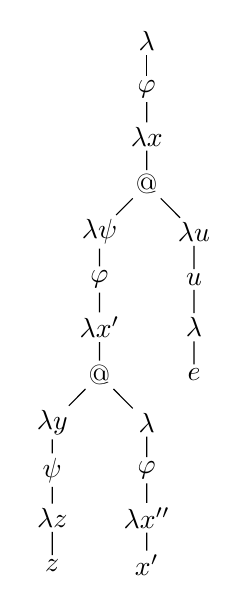
\begin{tikzpicture}[baseline=(root.base),level distance=4ex,inner ysep=0.5mm,sibling distance=12mm]
\node (root) {$\lambda$}
child {node {$\varphi$}
    child {node {$\lambda x$}
        child {node {$@$}
           child{node {$\lambda\psi$}
               child{node {$\varphi$}
                   child{node {$\lambda x'$}
                       child{node {$@$}
                           child{node {$\lambda y$}
                               child{node {$\psi$}
                                   child{node {$\lambda z$}
                                       child{node {$z$}}
                                   }
                               }
                           }
                           child{node {$\lambda$}
                               child{node {$\varphi$}
                                   child{node {$\lambda x''$}
                                       child{node {$x'$}}
                                   }
                               }
                           }
                       }
                   }
               }
           }
           child{node {$\lambda u$}
               child{node {$u$}
                   child{node {$\lambda$}
                       child{node {$e$}}
                   }
               }
           }
        }
    }
};
\end{tikzpicture}
\hspace{2cm} &
\vspace{1cm}
\begin{asparablank}
\item $t = \Pstr[0.7cm]{(n0){\lambda }\ (n1-n0){\varphi}\ (n2-n1){\lambda x}\ (n3){@}\ (n4-n3){\lambda \psi}\ (n5-n0){\varphi}\ (n6-n5){\lambda x'}\ (n7){@}\ (n8-n7){\lambda y}\ (n9-n4){\psi}\ (n10-n3){\lambda u}\ (n11-n10){u}\ (n12-n9){\lambda z}\ (n13-n12){z}\ (n14-n11){\lambda }\ }$
\item $\oview{t} = \Pstr[0.7cm]{(n0){@}\ (n1-n0){\lambda \psi}\ (n2-n1){\psi}\ (n3-n0){\lambda u}\ (n4-n3){u}\ (n5-n2){\lambda z}\ (n6-n5){z}\ (n7-n4){\lambda }\ }$
\item $\oview{t}\filterplus r_0 = \Pstr[0.7cm]{(n0){\lambda \psi}\ (n1-n0){\psi}\ (n2-n1){\lambda z}\ (n3-n2){z}\ }$

\item $t\filterplus r_0 = \Pstr[0.7cm]{(n0){\lambda \psi}\ (n1-n0){\varphi}\ (n2-n1){\lambda x'}\ (n3){@}\ (n4-n3){\lambda y}\ (n5-n0){\psi}\ (n6-n5){\lambda z}\ (n7-n6){z}\ }$
\item $\oview{ t \filterplus r_0 } = \Pstr[0.7cm]{(n0){\lambda \psi}\ (n1-n0){\psi}\ (n2-n1){\lambda z}\ (n3-n2){z}\ }$.
\end{asparablank}
\end{tabular}
\end{example}


\begin{example}
Take the term $e:o \vdash
    (\lambda f g . f (\lambda b . f (\lambda b'. b) (\lambda a' . a' e))
                        (\lambda a . a e))
    (\lambda x y . y (\lambda h . x (h e)) e) e$. Take the traversal:
$$t = \Pstr[1cm]{{\lambda }\ (n1){@}\ (n2-n1){\lambda f g}\ (n3-n2){f}\ (n4-n1){\lambda x y}\ (n5-n4){y}\ (n6-n3){\lambda a}\ (n7-n6){a}\ (n8-n5){\lambda h}\ (n9-n4){x}\ (n10-n3){\lambda b}\ (n11-n2){f}\ (n12-n1){\lambda x y}\ (n13-n12){y}\ (n14-n11){\lambda a'}\ (n15-n14){a'}\ (n16-n13){\lambda h}\ (n17-n12){x}\ (n18-n11){\lambda b'}\ (n19-n10){b}\ (n20-n9){\lambda }\ (n21-n8){h}\ }$$
then we have the following relations:
\smallskip

\begin{tabular}{lp{6cm}}
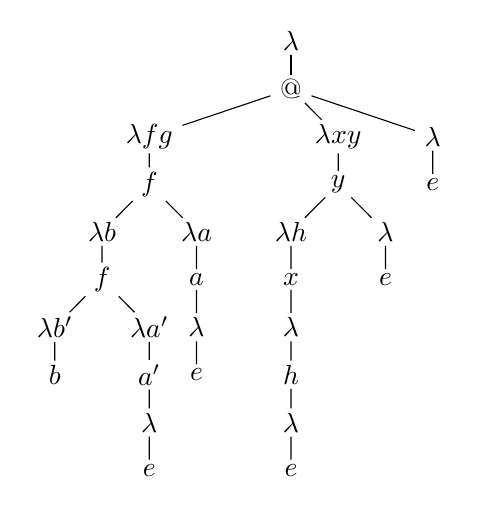
\begin{tikzpicture}[baseline=(root.base),level distance=4ex,inner ysep=0.5mm,sibling distance=12mm]
\node (root) {$\lambda$}
child {node {$@$}
    child {node {$\lambda f g$}
        child {node {$f$}
           child{node {$\lambda b$}
               child{node {$f$}
                   child{node {$\lambda b'$}
                       child{node {$b$}}
                   }
                   child{node {$\lambda a'$}
                       child{node {$a'$}
                           child{node {$\lambda$}
                               child{node {$e$}}
                           }
                       }
                   }
               }
           }
           child{node {$\lambda a$}
             child{node {$a$}
               child{node {$\lambda$}
                   child{node {$e$}}
               }
             }
           }
        }
    }
    child[missing]{}
    child {node {$\lambda x y$}
        child {node {$y$}
           child{node {$\lambda h$}
               child{node {$x$}
                   child{node {$\lambda$}
                       child{node {$h$}
                           child{node {$\lambda$}
                               child{node {$e$}}
                           }
                       }
                   }
               }
           }
           child{node{$\lambda$}
               child{node {$e$}}
           }
        }
    }
    child{node {$\lambda$}
       child{node {$e$}}
    }
};
\end{tikzpicture}
\hspace{0.5cm} &
\begin{asparablank}
\item $\oview{t} = \Pstr[0.7cm]{(n0){@}\ (n1-n0){\lambda f g}\ (n2-n1){f}\ (n3-n0){\lambda x y}\ (n4-n3){y}\ (n5-n2){\lambda a}\ (n6-n5){a}\ (n7-n4){\lambda h}\ (n8-n7){h}\ }$
\item $\oview{t}\filterplus r_0 = \Pstr[0.7cm]{(n0){\lambda f g}\ (n1-n0){f}\ (n2-n1){\lambda a}\ (n3-n2){a}\ }$
\item $t\filterplus r_0  = \Pstr[0.7cm]{(n0){\lambda f g}\ (n1-n0){f}\ (n2-n1){\lambda a}\ (n3-n2){a}\ (n4-n1){\lambda b}\ (n5-n0){f}\ (n6-n5){\lambda a'}\ (n7-n6){a'}\ (n8-n5){\lambda b'}\ (n9-n4){b}\ }$
\item $\oview{ t \filterplus r_0 } = \Pstr[0.7cm]{(n0){\lambda f g}\ (n1-n0){f}\ (n2-n1){\lambda a}\ (n3-n2){a}\ (n4-n1){\lambda b}\ (n5-n4){b}\ }$.
\end{asparablank}
\end{tabular}
\end{example}

\subsubsection{Subterm projections are sub-traversals}

We are now in a position to prove an important result that will require us to use all the lemmas and propositions from the previous two sections:
\begin{proposition}[Subterm projections are sub-traversals]
    \label{prop:trav_projection}
    Let $t \in \travset(M)$. For any occurrence $r_0$ in $t$ of some lambda node
    $r'\in N_\lambda$ we have $t\filterplus r_0 \in \travset(M^{(r')})$.
\end{proposition}
\proof
    We proceed by induction on the traversal rules. The base cases \rulenamet{Empty} and
    \rulenamet{Root} are trivial. \emph{Step case:} Take a traversal $t \in \travset(M)$ and suppose that the result holds for any traversal shorter than $t$.

    Suppose that $t^\omega$ does not appear in $t \filterplus r_0$ then
    the result follows by applying the induction hypothesis on $\ip(t)$.
    Suppose that $t^\omega$ appears in $t \filterplus r_0$ then we do a case analysis on the last traversal rule used to form $t$:
    \begin{itemize}
    \item \rulenamet{Lam}
        We have  $t = t' \cdot n$ with $t' = \ldots \cdot \lambda \overline{\xi}$. By the induction hypothesis, $t' \filterplus r_0 \in  \travset(M^{(r')})$.

        Since $n$ is a variable node appearing in $t\filterplus r_0$, by definition of $t\filterplus r_0$ its immediate predecessor
        $\lambda \overline{\xi}$ must occur in $t\filterplus r_0$ and therefore must be the last occurrence in $t'\filterplus r_0$. Thus we can use the rule \rulenamet{Lam} in $\tau(M^{(r')})$ to produce the traversal $u = (t'\filterplus r_0) \cdot n$ of $M^{(r')}$.

        We have $t \filterplus r_0 = (t'\filterplus r_0) \cdot n$, but in order to state that $u = t \filterplus r_0$ it remains to prove that $n$ has the same link in $t \filterplus r_0$ and in $u$.

        Suppose $n \in N_@ \union N_\Sigma$ then $n$ has no justifier in both $u$ and $t\filterplus r_0$. Otherwise $n \in N_{\sf var}$. Let us write $m_u$ to denote the occurrence in $t$ of $n$'s justifier in $u$, $m_t$ for the occurrence in $t$ of $n$'s justifier in $t$, and $m$ for the occurrence in $t$ of $n$'s justifier in $t \filterplus r_0$. We want to show that $m_u = m$.
        By the rule \rulenamet{Var}, $m_u$ is defined as the only occurrence of $n$'s enabler in $\pview{t'\filterplus r_0}$ and $m_t$ is the only occurrence of $n$'s enabler in $\pview{t'}$.

        If $r_0$ occurs before $m_t$ then by Lemma \ref{lem:pviewproj_traversal}(ii), $m_t$ appears in $t \filterplus r_0$ thus by definition of $\_ \filterplus$ we have $m = m_t$. Moreover, since $m_t$ appears in $t\filterplus r_0$, it must appear
        after $r_0$ by Lemma \ref{lem:pviewproj_traversal}(i.a), thus since it is in the P-view at $t'$, it must be
        in $\pview{t}_{\suffixof r_0}$ which is equal to $\pview{t'\filterplus r_0}$ by Lemma \ref{lem:pviewproj_traversal}(i.b)
        Hence we necessarily have $m_u = m_t$ (since $r'$ occurs only once in the P-view $\pview{t'\filterplus r_0}$).

        If $r_0$ occurs after $m_t$ then $m_t$ does not appear in $t\filterplus r_0$ thus $m = r_0$ by definition of $\_ \filterplus$. Moreover by Lemma \ref{lem:pviewproj_traversal}(i), $n$'s binder occurs in the path from $r'$ to the root $\theroot$. Thus $n$ is a free variable in $\tau(M^{(r')})$ and consequently the only enabler of $n$ occurring in $\pview{t'\filterplus r_0}$ is necessarily $r_0$: $m_u = r_0$.

        This proves the equality $t \filterplus r_0 = u$ and thus $t \filterplus r_0$ is a valid traversal of $M^{(r')}$.

    \item \rulenamet{App} $t = \ldots \cdot \lambda \overline{\xi} \cdot @ \cdot n$.
        Since $n$ appears in $t\filterplus r_0$, so does $@$ (by definition of $t\filterplus r_0$). Hence @ is the last occurrence in $t'\filterplus r_0$. By the induction hypothesis, $t' \filterplus r_0$ is a traversal of $\tau(M^{(r')})$ therefore we can use the rule \rulenamet{App} in $\tau(M^{(r')})$ to produce the traversal $(t'\filterplus r_0) \cdot n = t \filterplus r_0$ of $M^{(r')}$.


    \item \rulenamet{Value^{@\mapsto\lambda}} Take \Pstr[0.5cm]{t = t' \cdot (lmd){\lambda
        \overline{\xi}} \cdot (x){@}  \ldots  (xv-x,50:v){v}_@  \cdot
        (lmdv-lmd,30:v){v}_{\lambda \overline{\xi}} }.

        The occurrence $v_{\lambda \overline{\xi}}$ appears
        $t\filterplus r_0$ therefore since $r_0$ is not a lambda
        node, its justifier $\lambda \overline{\xi}$ also appear in
        $t\filterplus r_0$. Moreover since $@$ and $v_@$ are her.\
        just.\ by $\lambda \overline{\xi}$, they must also appear in
        $t\filterplus r_0$.

        By the induction hypothesis $t' \filterplus r_0$ is a
        traversal of $\tau(M^{(r')})$ therefore since the occurence
        $\lambda \overline{\xi}$, @, $v_@$, $v_{\lambda
        \overline{\xi}}$ all appear in $t\filterplus r_0$ we can use
        the rule \rulenamet{Value^{@\mapsto\lambda}} in $M^{(r')}$
        to form the traversal $(t'\filterplus r_0) \cdot n = t
        \filterplus r_0$ of $M^{(r')}$.

    \item \rulenamet{Value^{\lambda\mapsto @}}
          Take \Pstr[0.7cm]{t = t' \cdot (app){@} \cdot
        (lz-app,60){\lambda \overline{z}} \ldots
        (lzv-lz,60:v){v}_{\lambda \overline{z}} \cdot
        (appv-app,45:v){v}_@}. Again, since $v_@$ appears in $t
        \filterplus r_0$, necessarily the occurrences @, $\lambda
        \overline{z}$, $v_{\lambda \overline{z}}$ and $v_@$ must all
        appear in $t \filterplus r_0$. Hence using the induction
        hypothesis and the rule
        \rulenamet{Value^{\lambda\mapsto @}} in $M^{(r')}$ we
        obtain that $t \filterplus r_0$ is a traversal of
        $M^{(r')}$.

    \item \rulenamet{Value^{{\sf var}\mapsto\lambda}} Take \Pstr[0.5cm]{t = t' \cdot (lmd){\lambda
    \overline{\xi}} \cdot (x){x}  \ldots  (xv-x,50:v){v}_x  \cdot (lmdv-lmd,30:v){v}_{\lambda \overline{\xi}} }. Since $v_{\lambda \overline{\xi}}$ is in $t \filterplus r_0$, so must be $x$, $v_x$ and $\lambda \overline{\xi}$, by definition of $t \filterplus r_0$. Hence we can use the I.H.\ to form the traversal $t \filterplus r_0$ of $M^{(r')}$.

   \item \rulenamet{InputValue} Take \Pstr[0.4cm]{t =
    t_1 \cdot (x){x} \cdot t_2 \cdot (xv-x,38:v){v_x} } for some
    $v \in \mathcal{D}$ where $x$ is the pending node in $t_1 \cdot x \cdot t_2$ and $x \in N_{\sf var}^{\theroot\vdash}$.

    Since $v_x$ appears in $t\filterplus r_0$, so does $x$ hence
    by Lemma \ref{lem:projplus_pendingnode}, $x$ is also the
    pending node in $(t_1 \cdot x \cdot t_2)\filterplus r_0$.
    Furthermore since $M^{(r')}$ is a subterm of $M$, $x$ is
    necessarily an input-variable node in $\tau(M^{(r')})$.
    Hence we can conclude using the I.H.\ and the rule
    \rulenamet{InputValue}.

    \item \rulenamet{InputVar}  Take $t =  t' \cdot n$ where $n \in N_\lambda$ points to an occurrence of its parent node $y \in N_{\sf var}^{\theroot\vdash}$ in $\oview{t}$.
    By Lemma \ref{lem:ifin_projplus_so_does_justifier}(a), $y$
    must also appear in $t\filterplus r_0$, therefore $y$ also
    occurs in $\oview{t\filterplus r_0} \subseqof
    \oview{t}\filterplus r_0$. Hence we can conclude using the
    rule \rulenamet{InputVar} in $M^{(r')}$.


    \item \rulenamet{Var}
    Take \Pstr[0.6cm]{ t = t' \cdot (p){p} \cdot (lx){\lambda
        \overline{x}} \ldots (x-lx,30:i){x_i}  \cdot
        (letai-p,40:i){\lambda \overline{\eta_i}} } for some
        variable $x_i$ in $N_{\sf var}^{@\vdash}$.
    If $\lambda \overline{\eta_i}$ is the occurrence $r_0$ then
    the traversal $t\filterplus r_0 = r_0$ can be formed using
    the rule \rulenamet{Root}.

    Suppose that $\lambda \overline{\eta_i}$ is not the occurrence $r_0$. Then both $\lambda \overline{\eta_i}$ and its justifier $p$ must appear in $t\filterplus r_0$. The nodes $\lambda
    \overline{x}$ and $x_i$, however, do not necessarily appear in    $t\filterplus r_0$.

    Consider the node @ that initiates the thread of $\lambda \overline{\eta_i}$.

    \begin{compactitem}
    \item Suppose that $r_0$ precedes @ in $t$ then
    by Lemma \ref{lem:thread_projplus}(i), the nodes $\lambda
    \overline{\eta_i}$, $p$, $\lambda \overline{x}$ and $x_i$ as
    well as @ all appear in $t\filterplus r_0$. Moreover since @
    appear in $t\filterplus r_0$, it must be an occurrence of an
    application node that appear in the subtree rooted at $r'$
    thus $@ \in N_{\sf var}^{r'\vdash}$.  Hence we can use the
    use the rule \rulenamet{Var} in $M^{(r')}$ to form the
    traversal $t \filterplus r_0$ of $M^{(r')}$.

    \item Suppose that @ precedes $r_0$ in $t$ then
    by Lemma \ref{lem:thread_projplus}(ii), $p$ is necessarily
    an input variable node in $\tau(M^{(r')})$.

    We have $p \in \oview{t} \filterplus r_0 \subseqof \oview{t\filterplus r_0}$ by Proposition \ref{prop:oview_trav_projection}. Furthermore we can easily check that the last node in $\ip(t\filterplus r_0)$ is necessarily in $N_{\sf var} \union L_\lambda$ (using alternation and the fact that if an occurrence in $N_\lambda \union L_{\sf var} \union L_@ \union L_\Sigma \union N_@ \union N_\Sigma$ appears in $t\filterplus r_0$ then so does its immediate successor). Hence we can make use of the rule \rulenamet{InputVar} in $M^{(r')}$ (in its alternative form) to produce the traversal $t \filterplus r_0$ of $M^{(r')}$.
    \end{compactitem}

    \item \rulenamet{Value^{\lambda\mapsto{\sf var}}} Take \Pstr[0.7cm]{t = t' \cdot (y){y} \cdot (lmd){\lambda \overline{\xi}} \ldots (lmdv-lmd,30:v){v}_{\lambda \overline{\xi}}  \cdot (vy-y,50:v){v}_y } for some variable $y$ in $N_{\sf var}^{@\vdash}$.

    The proof is similar to the previous case using the rule \rulenamet{InputValue} instead of \rulenamet{InputVar} in the second subcase.

    \item \rulenamet{\Sigma}/\rulenamet{\Sigma\mbox{\sf-var}} The proof is similar to the case \rulenamet{App} and \rulenamet{Var}.

    \item \rulenamet{\Sigma\mbox{\sf-Value}} The proof is similar to the case \rulenamet{Value^{\lambda\mapsto{\sf var}}}. \qed
  \end{itemize}
% end of proof

The following Lemma will become useful in the proof of the Correspondence Theorem:

\begin{lemma} \label{lem:tstarproj_eq_tprojplusstar} Let $t$ be a traversal and $r_0$ be an occurrence of a
lambda node $r'$. We have
\begin{equation*}
(t\filterplus r_0)^\star = t^\star \filter V^{(r')} \filter r_0\ .
\end{equation*}
\end{lemma}
\proof By the previous Lemma, $t\filterplus r_0$ is indeed a
traversal (of $\tau(M^{(r')})$) thus the expression ``$(t\filterplus
r_0)^\star$'' is well-defined. We show the result by induction on
$t$: It is true for the empty traversal. Take $t=t'\cdot n$.

If $n$ belongs to $V_@ \union V_\Sigma$ then
\begin{align*}
((t' \cdot n) \filterplus n_0)^\star &= (t' \filterplus n_0)^\star \cdot
                \left\{
                  \begin{array}{ll}
                    n, & \hbox{if $n$ appears in $t\filterplus n_0$;} \\
                    \epsilon, & \hbox{otherwise.}
                  \end{array}
                \right.
 \\
\mbox{and } ((t' \cdot n)^\star \filter V^{(r')}) \filter n_0 &=
(t'^\star \filter V^{(r')}) \filter n_0
\cdot
                \left\{
                  \begin{array}{ll}
                    n, & \hbox{if $n$ is her.\ just.\ by $n_0$ in $t^\star\filter V^{(r')}$;} \\
                    \epsilon, & \hbox{otherwise.}
                  \end{array}
                \right.
\end{align*}
Since $t^\omega \not\in V_@ \union V_\Sigma$, by Lemma
\ref{lem:intfilterstar_iff_hjintstarfiltersubtree} we have that $n$
is her.\ just.\ by $n_0$ in $t^\star\filter V^{(r')}$ if and only if
$n$ appears in $t\filterplus n_0$. Hence we can conclude using the
I.H.\ on $t'$.


If $n$ does not belong to $V_@ \union V_\Sigma$ then
\begin{align*}
((t' \cdot n) \filterplus n_0)^\star &= (t' \filterplus n_0)^\star \\
&= (t'^\star \filter V^{(r')}) \filter n_0 & \mbox{(by the I.H.\ on $t'$)} \\
&= ((t' \cdot n)^\star \filter V^{(r')}) \filter n_0 \ \qed
\end{align*}
% end of proof

Consequently, by Lemma \ref{lem:minus_at_plus_at}, if $t^\omega
\not\in V_@ \union V_\Sigma$ then $t \filterplus r_0 =
(t^\star\filter r_0) +\Sigma+@$.



\subsubsection{O-view and P-view projection with respect to the root}

\begin{lemma}[O-view projection with respect to the root]
\label{lem:oviewproj_wrt_theroot}
Let $t$ be a non-empty traversal of $M$
and $r$ denote the only occurrence of $\tau(M)$'s root in $t$. If
$t^\omega$ appears in $t\filter r$ then:
$$\oview{t\filter r} = \oview{t}\filter r = \oview{t} \ .$$
\end{lemma}
\begin{proof}
It follows immediately from the fact that, by Lemma \ref{lem:trav_oview_single_threaded}, all the occurrences in $\oview{t}$ belong to the same thread and therefore are all hereditarily justified by $r$.
\end{proof}

\begin{lemma}[P-view projection with respect to the root]
\label{lem:pviewproj_wrt_theroot}
Let $t$ be a non-empty traversal of $M$ and $r$ denote the only occurrence of $\tau(M)$'s
root in $t$. If $t^\omega$ appears in $t\filter r$ then:
$$ \pview{t} \filter r \subseqof \pview{t \filter r} \  .$$
\end{lemma}
\proof We just sketch the proof. We proceeds exactly in the same way
as for the proof of Proposition \ref{prop:oview_trav_projection}.
Again we establish an analogy between traversals and plays of game
semantics:
\begin{center}
\begin{tabular}{r|p{5cm}}
{\bf Traversal setting} & {\bf Game-semantic setting} \\
\hline\hline
Traversal $t$ & Play $s$ \\
Nodes in $n \in N_\lambda \union L_{\sf var} \union L_\Sigma \union L_@$ & O-moves $\omove$ \\
Nodes in $n \in N_{\sf var} \union L_\lambda \union N_@ \union N_\Sigma \union \{\diamond\}$ & P-moves $\pmove$\\
P-view $\pview{t}$  & P-view $\pview{s}$\\
O-view $\oview{t}$  & O-view $\oview{s}$\\
Occurrence $n$ her.\ just.\ by $r$ in $t$ & Occurrence $n \in B$ \\
Occurrence $n$ not her.\ just.\ by $r$ in $t$ & Occurrence $n \in A$ \\
\parbox[t]{6cm}{\raggedleft No notion of initiality: all nodes are considered to be non-initial.} & Distinction between initial and non-initial move.
\end{tabular}
\end{center}
Clearly the conditions (w1) to (w8) hold. Hence we can reuse Proposition 4.3 form \cite{hylandong_pcf} which gives the desired result. \qed
% end of proof
\bigskip

The downside of the previous result is that it does not give us an
equality. In the particular case where interpreted constants are
well behaved, however, if we consider the subsequence of a traversal consisting of unanswered nodes only, then we obtain a nice equality:
\begin{lemma}
\label{lem:betanf_wellbehavedconst_trav_pview_red} Suppose that $M$
is in $\beta$-normal form and all the $\Sigma$-constants are
well-behaved. Let $t$ be a non-empty traversal of $M$ and $r$ denote
the only occurrence of $\tau(M)$'s root in $t$. If $t$'s last
occurrence is not a leaf then
$$ \pview{t} \filter r = \pview{?(t) \filter  r }\ .$$
\end{lemma}
\proof By induction. It is trivial for the empty traversal. Step
case: consider a traversal $t$ and suppose that the property (i) is
verified for all traversal shorter than $t$. We first observe that
since $t$ contains at most a single occurrence $r$ of the root
$\theroot$, an occurrence $n$ in $t$ is hereditarily justified by
$r$ if and only if the corresponding node in $\tau(M)$ is
hereditarily enabled by $\theroot$. Thus $t\filter r = t \filter
N^{\theroot \vdash}$. Let us do a case analysis on $t$'s last node:
\begin{itemize}
\item $t^\omega \in N_@$. This case does not happen since $M$ is $\beta$-normal.

\item $t = t' \cdot n$ with $n \in N_{\sf var} \union N_\Sigma$ then $t'^\omega$ is not a leaf (otherwise $n$ would also be a leaf by rule \rulenamet{Value}) thus we can use the I.H.\ on $t'$:
    \begin{align*}
    \pview{t} \filter  r
        &= \pview{t' \cdot n} \filter  r & (\mbox{definition of } t)\\
        &= \pview{t'} \cdot n \filter  r  & (\mbox{P-view computation}) \\
        &= \pview{t'} \filter  r  \cdot (n \filter  r)            & (\mbox{def. of projection $\filter$}) \\
        &= \pview{?(t') \filter r} \cdot (n \filter  r)           & (\mbox{induction hypothesis}) \\
        &= \pview{?(t') \filter  r \cdot (n \filter  r) } & (\mbox{P-view computation, $n \in N_{\sf var} \union N_{\Sigma}$}) \\
        &= \pview{(?(t') \cdot n ) \filter  r }           & (\mbox{def. of projection $\filter$}) \\
        &= \pview{?(t) \filter  r  }
 & (\mbox{definition of } t).
    \end{align*}
\end{itemize}
Suppose that $t^\omega$ is a lambda node. There are three subcases:
\begin{itemize}
\item $t^\omega \in N^{@\vdash}_\lambda$. Since the term is in $\beta$-normal form, there is no
    @-node in $\tau(M)$ so the rules \rulenamet{App} and
    \rulenamet{Var} are unused, hence this case does not happen.

\item $t^\omega \in N^{N_\Sigma\vdash}_\lambda$. We have $t =  t' \cdot \rnode{m}{m} \cdot  u \cdot \rnode{lmd}{n}
    \link[nodesep=1pt]{30}{lmd}{m}$ with $n\in N^{N_\Sigma
    \vdash}_\lambda$ and $m \in N_{\sf var} \union N_\Sigma$.
    The occurrence $n$ is necessarily visited with a
    \rulenamet{\Sigma}-rule. Since, by assumption, these rules
    are well-behaved we have $?(u) = \epsilon$. Hence:
        \begin{align*}
        \pview{t} \filter  r
        &= \pview{t' \cdot \rnode{m}{m} \cdot u \cdot \rnode{n}{n}} \filter  r
               \link[nodesep=1pt]{60}{n}{m}                   & (\mbox{Def. of $t$})\\
        &= (\pview{t'} \cdot \rnode{m}{m} \cdot \rnode{lmd}{n}) \filter  r
               \link[nodesep=1pt]{60}{lmd}{m}                 & (\mbox{P-view computation}) \\
        &= \pview{t'} \filter  r                & (m, n \not\in N^{\theroot \vdash}) \\
        &= \pview{?(t') \filter  r }               & \mbox{(induction hypothesis)} \\
        &= \pview{ ?(t' \cdot \rnode{m}{m} \cdot \rnode{lmd}{n}) \filter r }
\link[nodesep=1pt,ncurv=0.7]{40}{lmd}{m}                                                          & (m, n \not\in N^{\theroot \vdash}) \\
        &= \pview{ ?(t' \cdot \rnode{m}{m} \cdot u \cdot \rnode{lmd}{n}) \filter r }
\link[nodesep=1pt,ncurv=0.7]{40}{lmd}{m}                                                          & (?(u)=\epsilon) \\
        &= \pview{ ?(t) \filter r }                & \mbox{(def. of $t$ \& $u = \epsilon$).}
        \end{align*}

\item $t^\omega \in N^{\theroot\vdash}_\lambda$. If $t=r$ then the result holds trivially.
%%%% THE PREVIOUS CASE MUST BE REPLACED BY THE FOLLOWING COMMENTED LINES IF THE CALCULUS
%%%% CONSIDERED ALLOWS THE USE OF THE TENSOR PRODUCT IN THE SYNTAX (in which case the traversals need to be redefine
%%%% to allow the root to be visited several times).
%\item If $t = t' \cdot r$ then we have:
%    \begin{align*}
%    \pview{t} \filter  r
%        &=  r \filter  r                         & (\mbox{def. P-view})\\
%        &=  r                                                & (\mbox{def. operator $\filter$})\\
%        &=  \pview{(t' \filter  r ) \cdot r }    & (\mbox{def. P-view})\\
%        &=  \pview{(t' \cdot r)  \filter  r }    & (\mbox{def. operator $\filter$})\\
%        &= \pview{t \filter  r }                & (\mbox{def. of } t).
%    \end{align*}
Otherwise $t =  t' \cdot \rnode{m}{m} \cdot u \cdot
\rnode{lmd}{n} \link[nodesep=1pt]{30}{lmd}{m}$ for some $n\in
    N^{\theroot \vdash}_\lambda$ and:
        \begin{align*}
        \pview{t} \filter  r
        &= \pview{t' \cdot \rnode{m}{m} \cdot u \cdot \rnode{n}{n}} \filter  r
               \link[nodesep=1pt]{40}{n}{m}                   & (\mbox{definition of } t)\\
        &= (\pview{t'} \cdot \rnode{m}{m} \cdot  \rnode{lmd}{n} ) \filter  r
               \link[nodesep=1pt]{60}{lmd}{m}                 & (\mbox{P-view computation}) \\
        &= \pview{t'} \filter  r \cdot \rnode{m}{m} \cdot  \rnode{lmd}{n}
               \link[nodesep=1pt]{60}{lmd}{m}                 & (m, n \in N^{\theroot \vdash}) \\
        &= \pview{?(t')\filter r}  \cdot \rnode{m}{m} \cdot  \rnode{lmd}{n}
               \link[nodesep=1pt]{60}{lmd}{m}                 & \mbox{(induction hypothesis)} \\
        &= \pview{ ?(t') \filter r \cdot \rnode{m}{m} \cdot (?(u) \filter r) \cdot \rnode{lmd}{n}}
\link[nodesep=1pt,ncurv=0.6]{35}{lmd}{m}                                                          & (\mbox{P-view computation}) \\
        &= \pview{ (?(t') \cdot \rnode{m}{m} \cdot\ ?(u) \cdot \rnode{lmd}{n}) \filter r }
\link[nodesep=1pt,ncurv=0.7]{35}{lmd}{m}                                                          & (m, n \in N^{\theroot \vdash}) \\
        &= \pview{ ?(t' \cdot \rnode{m}{m} \cdot u \cdot \rnode{lmd}{n}) \filter r }
\link[nodesep=1pt,ncurv=0.7]{35}{lmd}{m}                                                          & \mbox{($m$ and $n$ are unanswered)} \\
        &= \pview{ ?(t) \filter r }                & \mbox{(def. of $t$).} \qed
        \end{align*}
\end{itemize}
% end of proof





\section{Game semantics correspondence}
\label{sec:gamesemcorresp}

{\it Notations and assumptions:}
We work in the general setting of an applied
simply-typed $\lambda$-calculus with a given set of higher-order
constants $\Sigma$. The operational semantics of these constants is
given by certain reduction rules. We assume that a fully abstract
model of the calculus is provided by means of a category of
well-bracketed games. For instance, if $\Sigma$ consists
of the \pcf\ constants then we consider the traditional
category of games and innocent well-bracketed strategies
\cite{hylandong_pcf,abramsky94full}.
A strategy is commonly defined in the literature as a set of plays closed by
even-length prefixing. For our purpose, however, it is more convenient to represent strategies using \emph{prefix-closed} set of plays. This will spare us some considerations on the parity of traversal length when showing the correspondence between traversals and game semantics.
 For the rest of the section we fix a simply-typed term $\Gamma \vdash M :T$. We write $\sem{\Gamma \vdash M : T}$ for its strategy denotation (in the standard cartesian closed category of games and innocent strategies \cite{abramsky94full, hylandong_pcf}). We use the notation $\prefset(S)$ to denote the prefix-closure of the set $S$.

\subsection{Interaction game semantics}
\label{sec:interaction_semantics}

In standard game semantics, terms are denoted by strategies that are computed
inductively on the structure of the term: calculating the denotation of a term boils down to
performing the composition of strategies denoting some of its subterms. Strategy composition consists of a
CSP-like ``composition + hiding'' operation where all the internal moves are hidden.

It is possible to use an alternative notion of composition where the internal moves are not hidden.
Game model based on such notion of composition have appeared in the literature under the name \emph{revealed
semantics} (\cite{willgreenlandthesis})  and \emph{interaction semantics} (\cite{DBLP:conf/sas/DimovskiGL05}).
In such game models, the denotation is computed inductively on the syntax of the term as in the standard game semantics, but certain internal
moves may be uncovered after composition. There is not just one interaction semantics as one may desire to hide/uncover different internal moves.
Moreover, since the denotation is computed inductively on the syntax of the term, the denotation is necessarily sensitive to the syntax and therefore such model cannot provide a full abstraction of the language considered.
However this semantics will prove to be useful to identify a correspondence between the game semantics of a term
and the traversals of its computation tree.

This section presents a general setting in which interaction semantics can be defined.
At the end of the section we will provide an example of such interaction semantics that is
calculated inductively on the syntax of the $\eta$-long normal form of the term.

\subsubsection{Revealed strategies}

\begin{definition} \hfill
\begin{itemize}
\item We call \defname{interaction type tree} or just \defname{interaction type},
a tree whose leaves are labelled with \pcf\ simple types and
inner nodes are labelled with symbol in $\{ ;, \langle \_\ ,\_
\rangle, \Lambda \}$.


Nodes labelled $;$ and $\langle \_\ ,\_ \rangle$ are binary
nodes while nodes labelled by $\Lambda$ are unary nodes. If
$T_1$ and $T_2$ are interaction types we write $\langle T_1, T_2
\rangle$ to denote the interaction type obtained by attaching
$T_1$ and $T_2$ to a $\langle \_\ ,\_ \rangle$-node. Similarly
we use the notations $T_1 ; T_2$ and $\Lambda(T_1)$.

\item To every node we can associate a simple type and we write
    $type(T)$ to denote the type associated to the root node. We
    sometime write the type in exponent {\it e.g.} $T^{A\gamear
    B}$ if $type(T) = A\gamear B$. This type is determined by
    the structure of the tree as follows:
    \begin{itemize}
    \item If $T$ is a leaf then $type(T)$ is define as the type that labels the leaf;

    \item $type\ \Lambda(T_1^{A \gameprod B \gamear C}) = A \gamear (B \gamear C)$

    \item $type\ \langle T_1^{C \gamear A} , T_2^{C \gamear B} \rangle =
    C \gamear A \gameprod B$;

    \item $type\ T_1^{A \gamear B};T_2^{B \gamear C} = A \gamear C$.
    \end{itemize}

\end{itemize}
Note that it is straightforward to generalize the pairing operator to a $p$-tuple operator $\langle \Sigma_1, \ldots, \Sigma_p \rangle$ for $p\geq2$ (in which case the root of the interaction game has $p$ children).

For the interaction type tree to be well-defined, it is required
that types of children nodes are consistent with the meaning of the
parent node; for instance the two children nodes of a ;-node must be
of type $A\gamear B$ and $B\gamear C$.

\end{definition}


Let $T$ be an interaction type tree. Each node of type $A$ in $T$
can be mapped to the (standard) game $\sem{A}$. By taking the image
of $T$ across this mapping we obtain a tree whose leaves and nodes
are labelled by games. This tree, written $\revsem{T}$, is called
an \defname{interaction game}.

A \defname{revealed strategy} $\Sigma$ on the interaction game $\revsem{T}$ is a compositions of several standard strategies in which certain internal moves are not hidden. Formally:
\begin{definition}
A \defname{revealed strategy} $\Sigma$ on an interaction game $\revsem{T}$,
written $\Sigma: \revsem{T}$, is an annotated interaction type
tree $T$ where
\begin{itemize}
\item each leaf $\sem{A}$ of $T$ is annotated with a (standard) strategy $\sigma$ on the game
$\sem{A}$;
\item each $;$-node is annotated with two sets of indices $U_{\sf sup}, U_{\sf prof} \subseteq \nat$ called respectively the
\emph{superficial} and \emph{profound} uncovering indices.
\end{itemize}
\end{definition}

\begin{example}
The diagrams below represent an interaction type tree $T$ (left),
the corresponding interaction game $\revsem{T}$ (middle) and a
revealed strategy $\Sigma$ (right):
\begin{center}
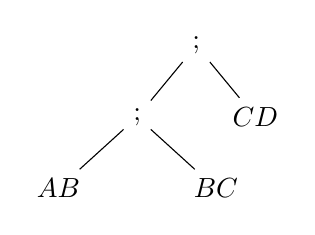
\begin{tikzpicture}[baseline=(root.base),level distance=6ex,sibling distance=15mm,level 2/.style={sibling distance=20mm}]
\node (root) {$;$}
child {node {$;$}
    child{node{$A\gamear B$}}
    child {node {$B\gamear C$}}
}
child{node{$C\gamear D$}};
\end{tikzpicture}
\hspace{5ex}
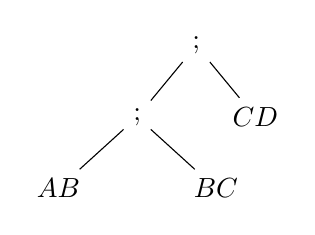
\begin{tikzpicture}[baseline=(root.base),level distance=6ex,sibling distance=15mm,
level 2/.style={sibling distance=20mm}]
\node (root) {$;$}
child {node {$;$}
    child {node {$\sem{A\gamear B}$}}
    child {node {$\sem{B\gamear C}$}}
}
child{node{$\sem{C\gamear D}$}};
\end{tikzpicture}
\hspace{5ex}
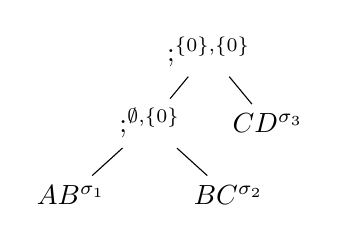
\begin{tikzpicture}[baseline=(root.base),level distance=6ex,sibling distance=15mm,
level 2/.style={sibling distance=20mm}]
\node (root) {$;^{\{0\},\{0\}}$}
child {node {$;^{\emptyset,\{0\}}$}
    child {node {$A\gamear B^{\sigma_1}$}}
    child {node {$B\gamear C^{\sigma_2}$}}
}
child{node{$C\gamear D^{\sigma_3}$}};
\end{tikzpicture}
\end{center}
\end{example}
A revealed strategy can also be written as an expression, for
instance the strategy represented above is given by the expression
$\Sigma = (\sigma_1 ;^{\emptyset,\{0\}} \sigma_2) ;^{\{0\},\{0\}} \sigma_3$.


The intuition behind this definition is that if a $;$-node has
children $\Sigma_1 : \revsem{A\gamear
B}$ and $\Sigma_2 : \revsem{B\gamear C}$ then the two
sets of indices $U_{\sf sup}, U_{\sf prof}$ indicate which components of $B$ should be
uncovered when performing composition. The set $U_{\sf sup}$ permits one to uncover \emph{superficial} internal moves \ie those that are created by the top-level composition (of $\Sigma_1$ with $\Sigma_2$), while the set $U_{\sf prof}$ can be used to cover/uncover the \emph{profound} internal moves \ie those that are already present in the revealed strategies $\Sigma_1$ and $\Sigma_2$.
The precise definition of this uncovering will be unveiled in the definition of the \emph{uncovered positions} of a revealed strategy in
the next paragraph.

\subsubsection{Uncovered play}

The analogous of a play in the interaction semantics is called an
\emph{uncovered play}, it is a play containing internal moves. Each move may belong to several games
from different nodes of the interaction game.
The moves are implicitly tagged so that it is possible to retrieve in
which component of the arena of which node-game the move belongs to.

\begin{definition}
The \defname{set of possible moves} $M_T$ of an interaction game
$\revsem{T}$ is defined as $\mathcal{M}_T/\hspace{-0.5em}\sim_T$,
the quotient of the set $\mathcal{M}_T$ by the equivalence relation
$\sim_T \subseteq \mathcal{M}_T \times \mathcal{M}_T$ defined as follows:
For a single leaf tree $T$ labelled by a type $A$ we define
$\mathcal{M}_T = M_A$ and $\sim_T = id_{M_A}$. For other cases:
    \begin{align*}
        \mathcal{M}_{\Lambda(T)} &= \mathcal{M}_{T} + M_{type(\Lambda(T))}
    \\
        \sim_{\Lambda(T)} &= \left( \sim_{T}
        \union \left(type\ \Lambda(T) \leftrightarrow type\ T\right)
        \right)^\star
    \\
    \\
        \mathcal{M}_{\langle T_1^{C^1 \gamear A^1}, T_2^{C^2 \gamear B^2}\rangle}
        &= \mathcal{M}_{T_1} + \mathcal{M}_{T_2} + M_{C \gamear (A \gameprod B)}
    \\
         \sim_{\langle T_1^{C^1 \gamear A^1}, T_2^{C^2 \gamear B^2}\rangle} &= \left( \sim_{T_1}
        \union \sim_{T_2} \union (C^1 \leftrightarrow C) \union (C^2 \leftrightarrow C)
        \union (A^1 \leftrightarrow A) \union (B^2 \leftrightarrow B)
        \right)^\star
    \\
    \\
        \mathcal{M}_{T_1^{A \gamear B};T_2^{B \gamear C}} &=
            \mathcal{M}_{T_1} + \mathcal{M}_{T_2} + M_{A\gamear C}
        \\
         \sim_{T_1^{A^1 \gamear B^1};T_2^{B^2 \gamear C^2}} &= \left( \sim_{T_1}
        \union \sim_{T_2} \union (A^1 \leftrightarrow A)
        \union (B^1 \leftrightarrow B^2) \union (C \leftrightarrow C^2)
        \right)^\star
    \end{align*}
    where $A\leftrightarrow B$ denotes the canonical bijection between two isomorphic arenas $\sem{A}$ and $\sem{B}$; $R^\star$ denotes the smallest superset of the relation $R$ complete by transitivity, reflexivity and symmetry.
\end{definition}

We call \defname{internal move} of the game $\revsem{T}$, any $\sim$-class from $M_T$ that does not contain any move from $M_{type(T)}$. We denote the set of all internal moves by $M_T^{\sf int}$. The complement of $M_T^{\sf int}$ in $M_T$, called the set of \defname{external moves}, is denoted by
$M_T^{\sf ext}$.

For any subgame $A$ occurring in some node of the interaction game $T$, we write $M_{T,A}^{\sf int}$ (resp. $M_{T,A}^{\sf ext}$) for the subset of moves of $M_T^{\sf int}$ (resp. $M_T^{\sf ext}$) consisting of $\sim$-classes containing some move in $M_A$.
\smallskip

A \defname{justified interaction sequence} of moves on the interaction game $\revsem{T}$ is a sequence of moves from $M_T$ together with pointers where each move in the sequence except the first one has a link attached to it pointing to some preceding move in the sequence.


\begin{definition}[Projection]
\label{def:sub_interstrat_projection}
We define several projection operations
over justified interaction sequences. Let $s$ be a justified
sequence of moves on the interaction game $\revsem{T}$.
\begin{enumerate}[i.]
\item  Let $T'$ be a direct subtree of $T$. We define the projection $s\filter T'$ to be the subsequence of $s$ consisting of moves $\sim$-equivalent to some move in $M_{T'}$. This operation may cause a move to ``lose'' its pointer. This situation corresponds to
    $(s \cdot m) \filter T' = (s \filter T') \cdot m$ where $m$'s justifier does not appear in $s \filter T'$.
    In that case, a new link is reassigned to $m$ that points to the only occurrence of an initial
    $\sem{type(T')}$-move in $\pview{s \filter \sem{type(T')}}$ (where $s \filter \sem{type(T')}$ is defined in iii.).

    Note that since $M_T$ is a set of equivalence classes with respect to $\sim$, the projection operator $\_ \filter T'$ implicitly performs the ``retagging'' of the moves to the appropriate components of each game of the interaction game $\revsem{T'}$.

\item  Let $T'$ be a non-direct subtree of $T$.
    We define the projection $s\filter T'$ as  $(\ldots (s\filter T^0) \filter \ldots \filter T^{k-1}) \filter T^k$
    where $T=T^0$ and $T'=T^k$ and for every $1\leq l \leq k$, $T^l$ is a direct subtree of $T^{l-1}$.

\item Let $T'$ be some subtree of $T$ and $A$ be a sub-game of $\sem{type(T')}$. We define the projection operator $s\filter A$ to be the subsequence of $s\filter T'$ consisting of the $\sim$-classes that contain some move in $M_A$.

\item For any initial move $m$ of the game $\sem{type(T)}$ occurring in $s$, $s \filter m$ is the subsequence of $s$ consisting of moves that are \emph{hereditarily justified} by that particular occurrence of $m$ in $s \filter type(T)$.
% NOTE: it is important to precise ``in $s \filter type(T)$'' because $s$'justification
% pointers differs depending on the sub-interaction game considered.
\end{enumerate}
By extension, we also define these operations on sets of justified interaction sequences.
\end{definition}


\begin{definition}[Legal uncovered positions] We recall
that in the standard game semantics, the set of legal positions
$L_A$ of a game $A$ is the set of justified sequences of moves from
$M_A$ respecting visibility and alternation. We define the set of
\defname{legal uncovered position} $L_T$ of an interaction game $\revsem{T}$ as
follows:
    \begin{itemize}
    \item If $T$ is a leaf annotated by a type $A$ then $L_T =
    L_A$;
    \item If $T$ is a unary node with child node $T'$ then:
    $$L_T = \{ s \in JustSeq(T) \ | \ s \filter type(T) \in L_{type(T)} \zand  s \filter T' \in L_{T'} \} \ ;$$
    \item If $T$ is a binary node with children nodes $T_1$ and $T_2$ then:
    $$L_T = \{ s \in JustSeq(T) \ | \ s \filter type(T) \in L_{type(T)} \zand  s \filter T_1 \in L_{T_1}
    \zand  s \filter T_2 \in L_{T_2} \} \ .$$
    \end{itemize}
    where $JustSeq(T)$ denotes the set of justified interaction sequences on
    $\revsem{T}$.
\end{definition}


We now define a revealed strategy by means of a set of uncovered positions the interaction game.
The set of positions of an interaction strategy is computed from its constituent standard strategies using a bottom-up computation starting from the leaves of the tree representing the strategy. In particular, at each ;-node the composition operation of game semantics will be applied. In contrast with the standard game semantics, however, internal moves will not be all hidden. But in accordance with standard game semantics (see projection $\_ \filter A,C$ in \cite{abramsky:game-semantics-tutorial}), when composing $\Sigma_l:T_l^{A\gamear B}$ with $\Sigma_r:T_r^{B\gamear C}$, the justification pointers are readjusted as follows: if an initial A-move $a$ has link pointing to an initial B-move itself pointing to an initial C-move $c$ then it is replaced by a link pointing directly to $c$. Thus if we take any interaction position $u$ of $\Sigma_l ; \Sigma_r$, by taking the subsequence of $u$ consisting of nodes in $A$ and $C$ only (ignoring the moves in $B$ as well as the internal moves coming from compositions that took place at deeper level in the interaction semantics) then we obtain a valid \emph{standard} position of the standard strategy that underlies the interaction strategy $\Sigma_l ; \Sigma_r$.

Additionally, given a position of an interaction strategy $\Sigma$ and a sub-interaction strategy $\Sigma':T'$ of $\Sigma:T$,
we would like to be be able to obtain a valid position of $\Sigma'$.
At first this may seem problematic since during composition we have lost all the links going from initial A-moves to initial B-moves!
Fortunately, these can be retrieved easily. Indeed, take an interaction sequence $u \cdot a \in Int(A,B,C)$ where $a$ is an initial A-move,
then by P-visibility in the game $A\gamear B$, $a$ points to an initial B-move in $\pview{u\filter A,B}$. But the P-view, by definition, contain at most one initial B-move! Hence the original pointer associated to $a$ can just be retrieved from the P-view $\pview{u\filter A,B}$.
We now observe that this pointer-recovery procedure corresponds precisely to the way the projection operation was defined in Def.\ \ref{def:sub_interstrat_projection}. Consequently, for any position $u$ of $\Sigma_l ; \Sigma_r$ where $\Sigma_l:T_l$ and $\Sigma_r:T_r$,
the sequence $u\filter T_l$ is a valid position of $\Sigma_l$ and $u\filter T_r$ is a valid position of $\Sigma_r$.
More generally, this implies that for any subtree $\Sigma':T'$ of $\Sigma:T$, and any position $u$ of the interaction strategy $\Sigma$, $u\filter T'$ is a valid position of $\Sigma'$.


\begin{definition}
\label{dfn:revealedstrat}
The set of \defname{uncovered positions} of a revealed strategy is defined inductively on the
structure of the annotated interaction type tree underlying the
interaction strategy:
\begin{itemize}[-]
\item Leaf labelled with type $A$ and annotated by the strategy $\sigma$: The set of positions of the revealed strategy is precisely the set of positions of the standard strategy $\sigma$ (which we have taken to be prefix-closed).

\item Currying: $\Lambda(\Sigma' : \revsem{T'}) : \revsem{T} = \{ u \in L_T \ |  u \filter T' \in \Sigma'  \}$.

\item Pairing: $$\begin{array}{lcll}
\langle \Sigma_1 : \revsem{T_1}, \Sigma_2 : \revsem{T_2} \rangle : \revsem{T} &= \{ u \in L_T \ | &
   (u \filter T_1 \in \Sigma_1 \zand\ u \filter T_2 = \epsilon) \\
&&  \zor\  ( u \filter T_1 = \epsilon \zand u \filter T_2 \in \Sigma_2) \}
\end{array}$$
where $type(T_1) = C\gamear A$, $type(T_2) = C\gamear B$
and $type(T) = C\gamear A \gameprod B$.

\item Uncovered composition: Take $\Sigma_1 : \revsem{T_1}$ and $\Sigma_2 :\revsem{T_2}$ then $\Sigma_1\ \| \ \Sigma_2$ is defined on the game $\revsem{T}$ where
$type(T) = A \gamear C$, $type(T_1) = A \gamear B_0 \gameprod
\ldots \gameprod B_l$ and $type(T_2) = B_0 \gameprod \ldots
\gameprod B_l \gamear C$ as
\begin{align*}
\Sigma_1 \| \Sigma_2 = \{ u \in L_T  \ | \
& \ \ u \filter T_2 \in \Sigma_2 \\
& \zand\ \parbox[t]{8.5cm}{for all occurrence $m$ in $u$ of an initial
                $\sem{type(T_1)}$-move, $u \filter T_1 \filter m \in \Sigma_1$} \\
& \zand\ \parbox[t]{8.5cm}{for any initial $m$ in $A$, if $m$ is justified in $u \filter T_1$ by $b\in B_j$,
itself justified by $c \in C^2$ in $u \filter T_2$ then $m$ is justified by $c$ in $u$. \} }
\end{align*}

\item Partially covered composition:
$$ \Sigma_1\ ;^{U_{\sf sup},U_{\sf prof}}\ \Sigma_2 = \{ \cover(u,\{0..l\}\setminus U_{\sf sup}, \{0..l\}\setminus U_{\sf prof}) \ | \ u \in \Sigma_1 \| \Sigma_2 \}$$
where
$$\cover(u,C_{\sf sup},C_{\sf prof}) = u \filter  M_T \setminus \left( \Union_{j\in
C_{\sf sup}} \overbrace{M^{\sf ext}_{T_1,B_j} \union M^{\sf ext}_{T_2,B_j})}^{\hbox{superficial $B_j$-moves}}
\union
\Union_{j\in
C_{\sf prof}} \overbrace{M^{\sf int}_{T_1,B_j} \union M^{\sf int}_{T_2,B_j})}^{\hbox{profound $B_j$-moves}} \right)$$
Observe that $\Sigma_1 \| \Sigma_2 = \Sigma_1;^{\{0..l\},\{0..l\}} \Sigma_2$.
\end{itemize}
\end{definition}


In words, the \emph{uncovered composition}
$\Sigma_1 \|\ \Sigma_2$ is the set of uncovered plays obtained by performing the usual composition of the standard strategies underlying $\Sigma_1$ and $\Sigma_2$ while preserving the internal moves already in $\Sigma_1$ and $\Sigma_2$ as well as the internal move produced by the composition.

Whereas if $B$ is the product game $B_0
\gameprod \ldots \gameprod B_l$ then the \emph{partially covered composition}
$\Sigma_1 ;^{U_{\sf sup}, U_{\sf prof}} \Sigma_2$
only keeps the superficial internal moves from the component $B_k$ for some $k \in U_{\sf sup}$ and the profound internal moves from the component $B_k$ for some $k \in U_{\sf prof}$.
\smallskip



\begin{lemma}[Complete interaction sequence]
\label{lem:inter_complete}
Let $u$ be an interaction sequence of some interaction strategy $\Sigma : \revsem{T}$
and suppose that the standard strategy denoting the leaves of $\Sigma$ are all well-bracketed.

Then for any node game $A$ of $T$ and interaction sequence $u\in
\Sigma$ we have:
\begin{enumerate}[i.]
\item $u \filter A$ is well-bracketed;

\item If $u \filter type(T)$ is complete (all question moves answered) then
    $u \filter A$ is complete.
\end{enumerate}
\end{lemma}
\begin{proof}
By induction on the structure of the interaction game
$\revsem{T}$. The base case is trivial. We only treat composition,
the other cases being trivial: Let $ u \in \Sigma_1 ; ^U \Sigma_2$
for some $U \subseteq \nat$ with $\Sigma_1 : \revsem{T_1^{A\gamear
B}}$ and $\Sigma_2 : \revsem{T_2^{B\gamear C}}$.

i. During composition, pointers attached to answer moves are
preserved with respect to $\sim$ thus non-well-bracketing of
$u\filter A\gamear C$ implies either non-well-bracketing of
$u\filter A\gamear B$ or $u\filter B\gamear C$.

For ii., suppose $u \filter type(T) = \Pstr{(q)q\ u'\ (a-q)a }$. By
well-bracketing (i.) and since $q$ and $a$ belong to $C$ we must
have $u \filter B\gamear C = \Pstr{(q)q \ldots (a-q)a}$ thus $u
\filter B\gamear C$ is complete. Suppose that $u \filter A\gamear B$
is not complete, then its first move is unanswered, but since this
is a $B$-move, it must also occur unanswered in $u \filter B\gamear
C$ which is a contradiction since we have just prove that $u \filter
B\gamear C$ is complete. Thus $u \filter A\gamear B$ is also
complete.

The induction hypothesis permits to conclude.
\end{proof}
Consequently if $u\filter type(T)$ is complete then $u$ is maximal {\em i.e.~no move (and in particular no internal move) can be played after $u$}.

\subsubsection{Fully-revealed and syntactically-revealed semantics}

We call \emph{revealed semantics} any game model of a language in which a term is denoted by some revealed strategy as defined in the previous section. As we have already observed, depending on the internal moves that we wish to hide, we obtain different possible revealed strategies for a given term. Hence there is not a unique way to define a revealed semantics. In this section we give two examples of such semantics.

Let $\pi_i$ denote the $i^{th}$ projection strategy $\pi_i : \sem{X_1 \gameprod
\ldots \gameprod X_l} \gamear \sem{X_i}$.

\begin{definition}[The fully-revealed semantics]
\label{dfn:fully_revealed_semantics}
The \defname{fully-revealed game denotation} of $M$ written $\revsem{\Gamma \vdash M : A}$ is defined by structural induction on the \emph{$\eta$-long normal form of $M$}:
\begin{eqnarray*}
\revsem{\Gamma \vdash \alpha : o} &=&
\sem{\Gamma \vdash \alpha : o} \quad \mbox{where } \alpha \in \Gamma \union \Sigma,\\
\revsem{\Gamma \vdash \lambda \overline{\xi} . M  : A} &=& \Lambda^{|\overline{\xi}|}(\revsem{\Gamma, \overline{\xi} \vdash M : o })  \\
\revsem{\Gamma  \vdash x_i N_1 \ldots N_p :o} &=& \langle \pi_i, \revsem{\Gamma \vdash N_1 : A_1}, \ldots, \revsem{\Gamma \vdash N_p : A_p}  \rangle \| ev^p, \quad X_i = A_0 \\
\revsem{\Gamma \vdash f N_1 \ldots N_p : o} &=& \langle \revsem{\Gamma \vdash N_1 : A_1}, \ldots, \revsem{\Gamma \vdash N_p : A_p} \rangle\ \|\ \sem{f}, \quad f : A_0 \in \Sigma \\
\revsem{\Gamma \vdash N_0 \ldots N_p : o} &=& \langle \revsem{\Gamma \vdash N_0 : A_0}, \ldots, \revsem{\Gamma \vdash N_p : A_p}  \rangle\ \|\ ev^p
\end{eqnarray*}
where $\Gamma = x_1 : X_1 \ldots x_l : X_l$, $A_0 =
(A_1,\ldots,A_p,o)$ and $ev^p$ denotes the evaluation strategy with
$p$ parameters where $p\geq 1$.
\end{definition}

Figure \ref{fig:interaction_strategy_denotations} shows tree representations of the interaction games involved in the revealed strategy $\revsem{\Gamma \vdash M : A}$ for the two application cases. These two trees give us information about the constituent strategies involved in $\revsem{M}$. For instance the revealed strategy $\revsem{N_0}$ is defined on the interaction game $\revsem{T^{00}}$ whose root game is $A \gamear B_0$, and the strategy $ev$ is defined on the interaction game $\revsem{T^1}$ whose underlying tree is constituted of a single game-node $B_0 \gameprod \ldots \gameprod B_p \gamear o$ (thus plays of $ev$ do not contain any uncovered move).

    \begin{figure}[htbp]
       \begin{center}
\begin{tikzpicture}[baseline=(root.base),level distance=5ex,inner ysep=0.5mm,
level 1/.style={sibling distance=70mm},
level 2/.style={sibling distance=30mm}]
\node (root) {$\revsem{N_0 N_1 \ldots N_p :o}:T [A\gamear o]$}
child {node {$\langle \revsem{N_0}, \ldots, \revsem{N_p} \rangle:T^{0}[A\gamear B_0\gameprod \ldots \gameprod B_p]$}
    child{node {$\revsem{N_0}:T^{00}[A\gamear B_0]$}
       child[child anchor=north,level distance=1ex] {node[isosceles triangle,draw,anchor=north,shape border rotate=90]{\hspace*{20pt}}}
    }
    child {node {$\ldots$}}
    child{node {$\revsem{N_p}:T^{0p}[A\gamear B_p]$}
       child[child anchor=north,level distance=1ex] {node[isosceles triangle,draw,anchor=north,shape border rotate=90]{\hspace*{20pt}}}
    }
}
child{node{$ev:T^1[B_0 \gameprod \ldots \gameprod B_p \gamear o]$}};
\end{tikzpicture}
\bigskip

       \emph{Tree-representation of the revealed strategy $\revsem{\Gamma \vdash N_0 N_1 \ldots N_p :o}$.}
       \end{center}

       \begin{center}
\begin{tikzpicture}[baseline=(root.base),level distance=7ex,inner ysep=0.5mm,
level 1/.style={sibling distance=70mm},
level 2/.style={sibling distance=35mm}]
\node (root) {$\revsem{x_i N_1 \ldots N_p :o}:T [A\gamear o]$}
child {node {$\langle \revsem{N_0}, \ldots, \revsem{N_p} \rangle:T^{0}[A\gamear B_0\gameprod \ldots \gameprod B_p]$}
    child{node {$\pi_i:T^{00}[A\gamear B_0]$}}
    child{node {$\revsem{N_1}:T^{01}[A\gamear B_1]$}
       child[child anchor=north,level distance=1ex] {node[isosceles triangle,draw,anchor=north,shape border rotate=90]{\hspace*{20pt}}}
    }
    child {node {$\ldots$}}
    child{node {$\revsem{N_p}:T^{0p}[A\gamear B_p]$}
       child[child anchor=north,level distance=1ex] {node[isosceles triangle,draw,anchor=north,shape border rotate=90]{\hspace*{20pt}}}
    }
}
child{node{$ev:T^1[B_0 \gameprod \ldots \gameprod B_p \gamear o]$}};
\end{tikzpicture}
\bigskip

       \emph{Tree-representation of the revealed strategy $\revsem{\overline{x}:\overline{X}\vdash x_i N_1 \ldots N_p :o}$.}
       \end{center}
    \bigskip
    {\small
     Node labels are of the form $\Pi : T[G]$ where $\Pi$ is a strategy, $T$ is the corresponding interaction game and $G$
     is the standard game that lies at the root of $T$.

     Each game is annotated with a string $s \in \{ 0..p \}^*$ in the exponent to indicate the path from the root to the corresponding node in the tree. (The digits in $s$ tell the direction to take at each branch of the tree).

    The games $A$ and $B$ are given by:
    \begin{eqnarray*}
        A &=& X_1 \gameprod \ldots \gameprod X_n\\
        B &=& \underbrace{((B_1' \gameprod \ldots \gameprod B_p') \gamear o')}_{B_0} \gameprod B_1 \gameprod \ldots \gameprod B_p
    \end{eqnarray*}
   }
       \caption{Tree-representation of the revealed strategy in the application case.}
      \label{fig:interaction_strategy_denotations}
    \end{figure}

\begin{example}
Take the term $\lambda x . (\lambda f . f x) (\lambda y . y)$.
Its fully-revealed denotation is $$\Lambda ( \langle \sem{ x:X \vdash \lambda f . f
x : (o\typear o) \typear o} , \sem{ x:X \vdash \lambda y . y
: o \typear o} \rangle \| ev^2 ) \ .$$
\end{example}

Note that the set of fully-revealed strategy is not a category (composition is not associative and there is no identity  strategy).


\begin{definition}[Syntactically-revealed semantics]
\label{dfn:syntactic_revealed_semantics} The \defname{syntactically-revealed game denotation} of $M$ written $\syntrevsem{\Gamma \vdash M : A}$ is defined by structural induction on the \emph{$\eta$-long normal form of $M$}. The equations are the same as in definition \ref{dfn:fully_revealed_semantics} except for the third case:
\begin{eqnarray*}
\syntrevsem{\Gamma  \vdash x_i N_1 \ldots N_p :o} &=& \langle \pi_i, \syntrevsem{\Gamma \vdash N_1 : A_1}, \ldots, \syntrevsem{\Gamma \vdash N_p : A_p}  \rangle ; ^{\emptyset,\{1..p\}} ev^p, \quad X_i = A_0 \ .
\end{eqnarray*}
\end{definition}

The syntactically-revealed denotation differs from the fully-revealed one in that only certain internal moves are preserved during composition: when computing the denotation of an application joint by an @-node in the computation tree, all the internal moves are preserved.
When computing the denotation of
$\revsem{y_i N_1 \ldots N_p}$ for some variable $y_i$, however, we only preserve the internal moves of
$N_1$, \ldots, $N_p$ while omitting the internal moves produced by the copy-cat projection strategy denoting $y_i$.


\subsubsection{Relating the two revealed denotations}
    \label{subsub:defdelta}

    As one would expect, the two revealed denotations that we have just introduced are in fact isomorphic: there is a transformation that maps $\revsem{\Gamma \vdash M : A}$ to $\syntrevsem{\Gamma \vdash M : A}$ and another one mapping $\syntrevsem{\Gamma \vdash M : A}$ to $\revsem{\Gamma \vdash M : A}$. That is what we are about to show in this section.

    \paragraph{The two revealed denotations are isomorphic}

    Take a term $M$ of the form $x_i N_1 \ldots N_p$ (This is the only case where the two revealed denotations differ). We use the notations introduced in Figure \ref{fig:interaction_strategy_denotations}.
    We have $\revsem{\Gamma \vdash M : o} =  \Sigma \|  ev$ and $\syntrevsem{\Gamma \vdash M : o} =  \Sigma_s ;^{\emptyset,\{1..p\}} ev$ where $\Sigma = \langle \pi_i, \revsem{\Gamma \vdash N_1 : B_1}, \ldots, \revsem{\Gamma \vdash N_p : B_p} \rangle$ and $\Sigma_s = \langle \pi_i, \syntrevsem{\Gamma \vdash N_1 : B_1}, \ldots, \syntrevsem{\Gamma \vdash N_p : B_p} \rangle$. For both denotations, the compositions takes place on the game
    $$ X_1 \times \ldots \overbrace{((B_1'' \times \ldots \times B_p'') \typear o'')}^{X_i} \ldots \times X_n \stackrel\Sigma\longrightarrow \psframebox[linestyle=dashed]{ \overbrace{((B_1' \times \ldots \times B_p') \typear o')}^{B_0} \times B_1 \times \ldots \times B_p }\stackrel{ev}\longrightarrow o$$
    where the dashed-line frame contains the internal components of the game. We will represent the superficial internal moves using the symbols $\opmove$, $\pomove$, $\omove$, $\pmove$ for OP-move, PO-move, O-move and P-move respectively.

    In $\revsem{\Gamma \vdash M : o}$, all the internal moves (including the profound ones) from $B_k$ for $k\in \{0..p\}$ are preserved, whereas in $\syntrevsem{\Gamma \vdash M : o}$, the internal moves from $B_0$ as well as the superficial internal moves in $B_k$ for $k\in \{1..p\}$ are hidden.


    Clearly, $\syntrevsem{\Gamma \vdash M : o}$ can be obtained from $\Sigma_s \| ev$ and conversely. Every play $u$ of $\Sigma_s \| ev$ corresponds to the play of $\syntrevsem{\Gamma \vdash M : o}$ obtained by removing all the superficial $B_k$-moves from $u$; and for any $u \in \syntrevsem{\Gamma \vdash M : o}$, there is a unique play $v$ of $\Sigma_s \| ev$ ending with an external move such that we obtain $u$ back after removing the superficial internal moves from $v$.
    Hence by repeating the same argument recursively at every subterm of $M$ of the form $y_i N_1 \ldots N_p$, we obtain that
    there exists a reversible transformation mapping $\syntrevsem{\Gamma \vdash M : o}$ to $\revsem{\Gamma \vdash M : o}$.

    \paragraph{Recovering the fully-revealed semantics from the syntactically-revealed semantics}


    We now explicitly define the transformation that turns $\syntrevsem{\Gamma \vdash M : o}$ into $\revsem{\Gamma \vdash M : o}$. To achieve this, it suffices to define constructively the function mentioned in the previous paragraph which given an interaction play $u$ of $\syntrevsem{\Gamma \vdash M : o}$ returns $v$, the unique play of $\syntrevsem{\Gamma \vdash M : o}$ ending with an external move such that removing the superficial internal moves from $v$ gives us back $u$. Let us call $\delta$ this transformation.

    Let us analyse the structure of an interaction play of $\Sigma \|  ev$. The diagram in Figure \ref{fig:flowdiag_moves_interplay_varcase} gives us a precise description of the flow of an interaction play. The nodes of the diagram represent the moves. A node label is of the form $A,\alpha$ where $\alpha \in \{\omove,\pmove,\pomove,\opmove\}$: the first component is the game in which the move is played and the second indicates which player is making the move. The notation $X_i.B''_k$ is used to denote the sub-component $B''_k$ of $X_i$. The edges indicate the moves that are allowed in a given state of the game. The game starts at node $C,\omove$ which correspond to the initial move of the overall game. Each edge is labelled with the strategy that plays the corresponding move. For instance the edge $B_k,\pomove \stackrel{ev}\longrightarrow B_0,\opmove$ tells us that if $B_k,\pomove$ is the last move played then the evaluation strategy allows the other user to respond with the move $B_k,\pomove$. The copy-cat strategies are highlighted with dashed-edges.

    We observe that every (superficial) internal move played in some component $B_k$ for $k\in \{0..p\}$ is either a copy of a previous external move, or it is subsequently copied to a external component by the copy-cat strategy $ev$ or $\pi_i$.  For instance, the $\opmove$-moves from $B_0$ are copies by $ev$ of O-moves from $C$ and $\pomove$-moves from $B_k$ for $k \in \{1..p\}$; the $\pomove$-moves from $B_0$ are copies by $\pi_i$ of O-move from $X_i$; and $\opmove$-moves from $B_k$ for every $k \in \{1..p\}$ are copies by $ev$ of $\pomove$-moves from the components $B_k'$ of $B_0$.

    Moreover, each move on the diagram of Figure \ref{fig:flowdiag_moves_interplay_varcase} has either a single outgoing copy-cat edge in which case the following move is uniquely determined, or it has multiple out-going edges all labelled by $\Sigma$ in which case the strategy $\Sigma$ determines which moves will be played next.
    Hence for any two consecutive move in a play of $\syntrevsem{\Gamma \vdash M : o}$ we can uniquely recover all the internal moves occurring between the two moves in the corresponding play of $\revsem{\Gamma \vdash M : o}$ by following the arrows of the flow diagram.
    \begin{figure}
    \begin{center}
    $\psset{linewidth=0.5pt}
    \begin{psmatrix}[rowsep=15pt,colsep=2cm]%
          [name=B0_op]B_0, \opmove & & & [name=C_o] C, \omove \\
                      & [name=Xi_p] X_i, \pmove \\
                      & [name=XiBk_o] X_i.B_k'', \omove & [name=Xio_o] X_i.o'',\omove \\[0pt]
          [name=B0Bk_po] B_0.B'_k, \pomove & & [name=B0o_po] B_0.o',\pomove & [name=C_p] C,\pmove \\[0pt]
          [name=Bk_op]B_k,\opmove \\
          & [name=Xj_p]{X_j}_{j\neq i},\pmove \\
          & [name=Xj_o]{X_j}_{j\neq i},\omove \\[0pt]
          [name=Bk_po]B_k,\pomove
        \end{psmatrix}
    \ncline[linestyle=dashed]{->}{C_o}{B0_op}\nbput{ev}
    \ncline[linestyle=dashed]{->}{B0_op}{Xi_p}\naput{\pi_i}
    \ncline[linestyle=dashed]{->}{XiBk_o}{B0Bk_po}\nbput{\pi_i}\ncline[linestyle=dashed]{->}{Xio_o}{B0o_po}\naput{\pi_i}
    \ncline[linestyle=dashed]{->}{B0o_po}{C_p}\naput{ev}
    \ncline[linestyle=dashed]{->}{B0Bk_po}{Bk_op}\naput{ev}
    \ncarc[arcangle=45,linestyle=dashed]{->}{Bk_po}{B0_op}\naput{ev}
    % non-copycat moves
    \ncline{->}{Bk_op}{Bk_po}\naput{\Sigma}
    \ncline{->}{Bk_op}{Xj_p}\naput{\Sigma}
    \ncline[offset=4pt]{->}{Xj_p}{Xj_o}\naput{env}
    \ncline[offset=4pt]{->}{Xj_o}{Xj_p}\naput{\Sigma}
    \ncline{->}{Xj_o}{Bk_po}\naput{\Sigma}
    \ncline{->}{Xj_p}{XiBk_o}\naput{env}
    \ncline{->}{Xi_p}{XiBk_o}\nbput{env}
    \ncline{->}{Xi_p}{Xio_o}\naput{env}
    \nccurve[angleA=160,angleB=170]{->}{Bk_op}{Xi_p}\naput{\Sigma}
    \nccurve[angleA=40,angleB=-30]{<->}{Xj_o}{Xi_p}\nbput{\Sigma}
    $%
    \end{center}
    where $k\in\{1..p\}$ and $i,j \in \{1..n\}$.
    \caption{Flow-diagram for interaction plays of $\revsem{\Gamma \vdash x_i N_1 \ldots N_p}$.}
    \label{fig:flowdiag_moves_interplay_varcase}
    \end{figure}


\subsubsection{Revealed semantics versus standard game semantics}
\label{subsec:relating_revealed_and_standard_denotation}

In the standard semantics, given two strategies $\sigma : A
\gamear B$, $\tau : B \gamear C$ and a sequence $s \in
\sigma ; \tau$, it is possible to (uniquely) recover the
internal moves from the sequence $s$ that have been hidden during composition. The algorithm to obtain this unique uncovering, written ${\bf u}(s, \sigma, \tau)$, is given in \cite[part II]{hylandong_pcf}. By performing recursively this uncovering for every application occurring in a given term, one can completely uncover the internal moves from a play of the term's denotation.
Hence the revealed denotation can be recovered from the standard game denotation.

Conversely, the standard denotation can be obtained from the revealed denotation by filtering out all the internal moves:
\begin{eqnarray}
 \sem{\Gamma \vdash M : T} = \revsem{\Gamma \vdash M : T} \filter \sem{\Gamma \gamear T} \label{eqn:int_std_gamsem}
\end{eqnarray}
Of course, this equality remains valid if we use the syntactically revealed semantics instead of the fully revealed semantics.


Observe that the two set of plays $\revsem{\Gamma \vdash M : T}$ and $\sem{\Gamma \vdash M : T}$ are not in bijection.  Indeed, by definition the revealed denotation is prefix-closed therefore it also contains plays ending with an internal move. Thus the revealed denotation contains more plays than the standard denotation.

In fact, the set of plays $\sem{\Gamma \vdash M : T}$ is in bijection with the subset of $\revsem{\Gamma \vdash M : T}$ consisting of plays ending with an external move. Additionally, the set of complete plays of $\sem{\Gamma \vdash M : T}$ is in bijection with the set of complete interaction plays of $\revsem{\Gamma \vdash M : T}$.


\subsection{Relating computation trees and games}
In this paragraph we are interested in showing a relation between nodes of the computation tree and moves of the game arena.
Let us first get the insight from an example before giving the formal definition.
\subsubsection{Example}
Consider the following term $M \equiv \lambda f z . (\lambda g x . f (f x)) (\lambda y. y) z$ of type $(o \typear o) \typear o \typear o$.
Its $\eta$-long normal form is $\lambda f z . (\lambda g x . f (f x)) (\lambda y. y) (\lambda .z)$.
The following figure represents the computation tree of $M$ on the left and the
arena of the game $\sem{(o \typear o) \typear o \typear o}$ on the right:
\begin{center}
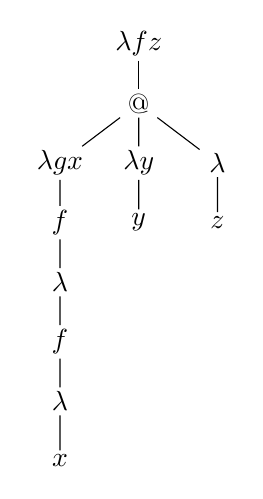
\begin{tikzpicture}[baseline=(root.base),level distance=5ex,inner ysep=0.5mm,sibling distance=10mm]
\node (root) {$\lambda f z$}
child {node {$@$}
    child {node {$\lambda g x$}
        child {node {$f$}
            child {node {$\lambda$}
                child {node {$f$}
                    child {node {$\lambda$}
                        child {node {$x$}}
                    }
                }
            }
        }
    }
    child {node {$\lambda y$}
           child {node {$y$}}
    }
    child {node {$\lambda$}
           child {node {$z$}}
    }
};
\end{tikzpicture}
\hspace{3cm}
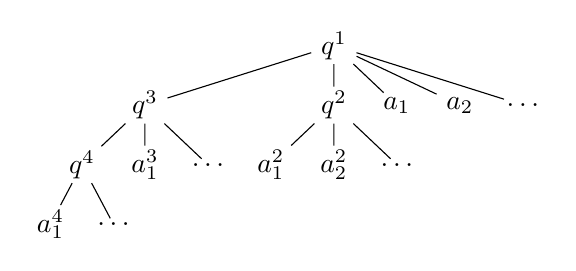
\begin{tikzpicture}[baseline=(root.base),level distance=5ex,inner ysep=0.5mm,sibling distance=8mm]
\node (root) {$q^1$}
child {node {$q^3$}
    child {node {$q^4$}
           child {node {$a_1^4$}}
           child {node {$\ldots$}}
    }
    child {node {$a_1^3$}}
    child {node {$\ldots$}}
    }
child[missing]{}
child[missing]{}
child {node {$q^2$}
       child {node {$a_1^2$}}
       child {node {$a_2^2$}}
       child {node {$\ldots$}}
    }
child {node {$a_1$}}
child {node {$a_2$}}
child {node {$\ldots$}};
\end{tikzpicture}
\end{center}

\newlength{\yNull}
\def\bow{\quad\psarc{->}(0,\yNull){1.5ex}{90}{270}}

The figure below represents the computation tree (left) and the
arena (right). The dashed line defines a partial function $\psi$
from the set of nodes in the computation tree to the set of moves.
For simplicity, we now omit answer moves when representing arenas.
\begin{center}
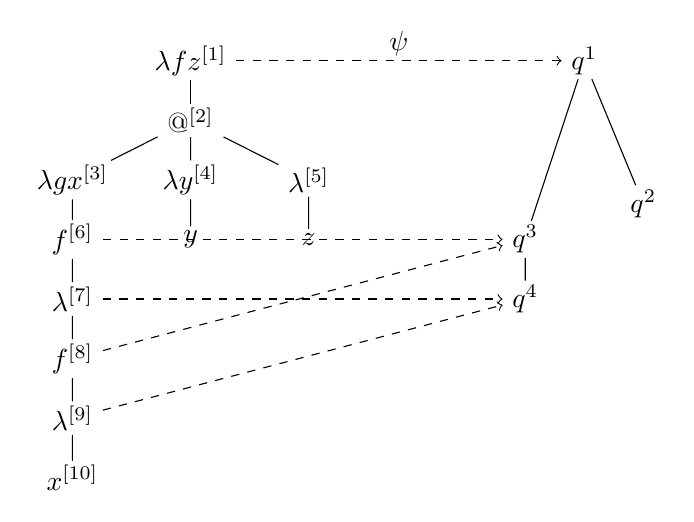
\begin{tikzpicture}[baseline=(root.base),level distance=5ex,inner ysep=0.5mm,sibling distance=15mm]
\path
node (root) {$\lambda f z^{[1]}$}
child{node {$@^{[2]}$}
    child{node {$\lambda g x^{[3]}$}
        child{node (f6) {$f^{[6]}$}
            child{node (l7) {$\lambda^{[7]}$}
                child{node (f8) {$f^{[8]}$}
                    child{node (l9) {$\lambda^{[9]}$}
                        child{node (l10) {$x^{[10]}$}}
                    }
                }
            }
        }
    }
    child {node {$\lambda y^{[4]}$}
           child {node {$y$}}
    }
    child {node {$\lambda^{[5]}$}
           child {node {$z$}}
    }
}
+(5cm,0)
node (q1){$q^1$}
child[level distance=15ex]{node(q3){$q^3$}
    child[level distance=5ex]{node(q4){$q^4$}}
    }
child[level distance=12ex]{node {$q^2$}};
\draw[dashed,->] (f6) -- (q3);
\draw[dashed,->] (f8) -- (q3);
\draw[dashed,->] (l7) -- (q4);
\draw[dashed,->] (l9) -- (q4);
\draw[dashed,->] (root) -- node[above]{$\psi$} (q1);
\end{tikzpicture}
\end{center}

Consider the justified sequence of moves $s \in \sem{M}$:
 $$s = \Pstr[12pt][5pt]{(q1){q}^1\ (q3-q1,60){q}^3\ (q4-q3,60){q}^4\ (q3b-q1){q}^3\ (q4b-q3b,60){q}^4\ (q2-q1,30){q}^2 }
\in \sem{M}$$

There is a corresponding justified sequence of nodes in the computation tree:
$$r = \Pstr[0.8cm]{
        (q1){\lambda f z} \cdot
        (q3-q1,60){f}^{[6]} \cdot
        (q4-q3,60){\lambda^{[7]}} \cdot
        (q3b-q1,60){f}^{[8]} \cdot
        (q4b-q3b,50){\lambda^{[9]}} \cdot
        (q2-q1,50){z} }$$
such that $s_i = \psi(r_i)$ for all $i < |s|$.

The sequence $r$ is in fact the reduction of the following
traversal:
$$t = \pstr[1.1cm]{ \nd(q1){\lambda f z} \cdot
            \nd(n2){@^{[2]}} \cdot \nd(n3-n2,60){\lambda g x^{[3]}} \cdot
            \nd(q3-q1,60){f}^{[6]} \cdot \nd(q4-q3,60){\lambda^{[7]}} \cdot
            \nd(q3b-q1,40){f}^{[8]} \cdot \nd(q4b-q3b,70){\lambda^{[9]}} \cdot
            \nd(n8-n3,35){x^{[10]}} \cdot
            \nd(n9-n2,30){\lambda^{[5]}} \cdot
            \nd(q2-q1,35){z}}
$$

By representing side-by-side the computation tree and the type arena of a term in $\eta$-normal form we have observed
that some nodes of the computation tree can be mapped to question moves of the arena.
In the next section, we show how to define this mapping in a systematic manner.

\subsubsection{Formal definition}

We now establish formally the relationship between games and
computation trees. We assume that a term $\Gamma \vdash M : T$ in $\eta$-long
normal form is given.

\emph{Notations:} We suppose that computation tree $\tau(M)$ is given by
a pair $(V,E)$ where $V$ is the set of vertices and $E \subseteq
V \times V$ is the parent-child relation. We have $V = N \union L$
where $N$ and $L$ are the set of nodes and value-leaves respectively.
Let $\mathcal{D}$ be the set of values of the base type $o$. If $n$
is a node in $N$ then the value-leaves attached to the node $n$ are
written $v_n$ where $v$ ranges in $\mathcal{D}$. Similarly, if $q$
is a question in $A$ then the answer moves enabled by $q$ are
written $v_q$ where $v$ ranges in $\mathcal{D}$.

\begin{definition}[Mapping from nodes to moves of the standard game-semantics]\hfill
\label{def:psi mapping}

    \begin{itemize}
    \item Let $n$ be a node in $N_\lambda \union N_{\sf var}$ and $q$ be a question move of some game $A$
such that $n$ and $q$ are of type $(A_1,\ldots,A_p,o)$ for some
$p\geq 0$. Let $\{ q^1, \ldots, q^p \}$ (resp.\  $\{ v_q \ | \ v \in \mathcal{D} \}$)
be the set of question (resp.\ answer) moves enabled by $q$ in $A$ (each $q^i$ being of type $A_i$).

We define the function $\psi^{n,q}_A$ from $V^{n \vdash}$
(the nodes from $V$ that are hereditarily enabled by $n$)
to moves of $A$ as:
        \begin{eqnarray*}
        \psi^{n,q}_A &=& \{ n \mapsto q \} \union  \{ v_n \mapsto v_q \ | \ v \in \mathcal{D} \}\\
         &&\union \left\{
                        \begin{array}{ll}
                          \Union_{m \in N_{\sf var} | n \vdash_i m} \psi^{m, q^i}_A, & \hbox{if $n\in N_{\lambda}$\ ;} \\
                          \Union_{i=1..p} \psi^{n.i, q^i}_A, & \hbox{if $n\in N_{\sf var}$\ .}
                        \end{array}
                      \right.
        \end{eqnarray*}

    \item Suppose $\Gamma = x_1:X_1, \ldots ,
    x_k:X_k$. Let $q_0$ denote $\sem{\Gamma\gamear T}$'s
    initial move\footnote{Arenas involved in the game semantics
    of simply-typed $\lambda$-calculus are all trees: they have
    a single initial move.} and suppose that the set of moves
    enabled by $q_0$ in $\sem{\Gamma\gamear T}$ is
     $\{ q_{x_1}, \ldots, q_{x_k}, q^1, \ldots, q^p \} \union \{
    v_q \ | \ v \in \mathcal{D} \}$ where each $q^i$ is of type
    $A_i$ and $q_{x_j}$ of type $X_j$.

    We define $\psi_M : V^{\theroot\vdash} \rightarrow
    \sem{\Gamma\gamear T}$ (or just $\psi$ if there is
    no ambiguity) as:
    \begin{eqnarray*}
     \psi_M = && \{ r \mapsto q_0 \}  \union  \{ v_r \mapsto v_{q_0} \ | \ v \in \mathcal{D} \}\\
& \union& \Union_{n \in N_{\sf var} | \theroot\vdash_i n} \psi^{n, q^i}_\sem{\Gamma\gamear T} \\
& \union& \Union_{n \in N_{\sf fv} | n \mbox{ \small labelled } x_j, j \in \{ 1..k \} } \psi^{n, q_{x_j}}_\sem{\Gamma\gamear T} \ .
    \end{eqnarray*}
    \end{itemize}
\end{definition}

It can easily be checked that the domain of definition of $\psi^{n,q}_A$
is indeed the set of nodes that are hereditarily enabled by $n$ and similarly,
the domain of $\psi_M$ is the set of nodes that are hereditarily enabled by
the root (this includes free variable nodes and nodes that are hereditarily enabled by free variable nodes).
Also, if $M$ is closed then we have $\psi_M = \psi^{\theroot,q_0}_{\sem{\gamear T}}$.
\smallskip

The construction of the function $\psi^{n,q}_A$, defined above, goes as follows. Let $p$ be the arity of the type of $n$ and $q$.
\begin{itemize}
\item If $p=0$ then $n$ is a dummy $\lambda$-node or a ground type variable: $\psi^{n,q}_A$ maps $n$ to the initial move $q$.

\item  If $p\geq 1$ and $n \in N_{\lambda}$ with $n$ labelled $\lambda \overline{\xi} = \lambda \xi_1 \ldots \xi_p$ then the sub-computation tree rooted at $n$ and the
 arena $A$ have the following forms (value-leaves and answer
 moves are not represented for simplicity):
\begin{center}
\begin{tikzpicture}[baseline=(root.base),level distance=5ex,sibling distance=15mm]
\node (root){$\lambda \overline{\xi}^{[n]}$} child{node{$\alpha$}child{node{}child[dotted]{node{}}}child{node{$\ldots$}}child{node{}child[dotted]{node{}}}}
+(7cm,0)
node (qlx){$q$} child{node{$q^1$} child[dotted]{node{}}child[dotted]{node{}}} child{node{$q^2$}child[dotted]{node{}}child[dotted]{node{}}} child{node{$\ldots $}} child{node{$q^p$}child[dotted]{node{}}child[dotted]{node{}}};
\draw[dashed,->] (root) -- node[fill=white]{$\psi_A^{n,q}$} (qlx) ;
\end{tikzpicture}
\end{center}
    For each abstracted variable $\xi_i$ there exists a
    corresponding question move $q^i$ of the same order in the
    arena. $\psi^{n,q}_A$ maps each free occurrence of $\xi_i$
    in the computation tree to the move $q^i$.

\item If $p\geq 1$ and $n\in N_{\sf var}$ then $n$ is labelled with a variable $x:(A_1,\ldots,A_p,o)$
with children nodes $\lambda \overline{\eta}_1$, \ldots,
$\lambda \overline{\eta}_p$. The computation tree $\tau(M)$
rooted at $n$ and the arena $A$ have the following forms:
\begin{center}
\begin{tikzpicture}[baseline=(root.base),level distance=5ex,sibling distance=15mm]
\node (root){$x^{[n]}$} child{node{$\lambda\overline\eta_1$}child[dotted]{node{}}}child{node{$\ldots$}}child{node{$\lambda\overline\eta_p$}child[dotted]{node{}}}
+(7cm,0)
node (qlx){$q$} child{node{$q^1$} child[dotted]{node{}}child[dotted]{node{}}} child{node{$q^2$}child[dotted]{node{}}child[dotted]{node{}}} child{node{$\ldots $}} child{node{$q^p$}child[dotted]{node{}}child[dotted]{node{}}};
\draw[dashed,->] (root) -- node[fill=white]{$\psi_A^{n,q}$} (qlx) ;
\end{tikzpicture}
\end{center}
    and $\psi^{n,q}_A$ maps each node $\lambda
    \overline{\eta}_i$ to the question move $q^i$.
\end{itemize}


\begin{example} For each of the following examples of term $\Gamma \vdash M :T$, we represent the
computation tree $\tau(M)$, the arena of the game  $\sem{\Gamma \gamear T}$, and
the function $\psi_M$ (in dashed lines):
\begin{compactitem}
\item $M = \lambda x^o . x$
\begin{center}
\begin{tikzpicture}[baseline=(root.base),level distance=5ex,sibling distance=15mm]
\node (root){$\lambda x$} child{node(x){$x$}}
+(5cm,0)
node (qlx){$q_{\lambda x}$} child{node(qx){$q_x$}};
\draw[dashed,->] (root) -- node[fill=white]{$\psi_M$} (qlx) ;
\draw[dashed,->]  (x) -- (qx);
\end{tikzpicture}
\end{center}

\item $M = \lambda f^{(o,o,o)} . f x y$
\begin{center}
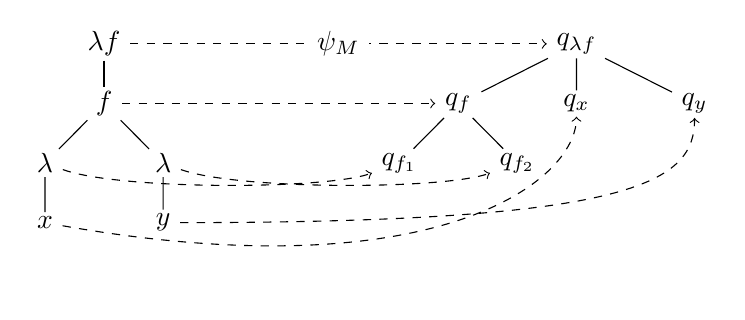
\begin{tikzpicture}[baseline=(root.base),level distance=5ex,inner ysep=0.5mm,sibling distance=15mm]
\path
node (root){$\lambda f$}
child{node(f){$f$}
 child{node(l1){$\lambda$} child{node(x){$x$}}}
 child{node(l2){$\lambda$} child{node(y){$y$}}}
}
+(6cm,0)
node (qlf){$q_{\lambda f}$}
child{node(qf){$q_f$}
    child{node(qf1){$q_{f_1}$}}
    child{node(qf2){$q_{f_2}$}}
    }
child{node(qx){$q_x$}}
child{node(qy){$q_y$}};
\draw[dashed,->] (root) -- node[fill=white]{$\psi_M$} (qlf);
\draw[dashed,->] (f) -- (qf);
\draw[dashed,->] (l1) .. controls +(-20:1cm) and +(200:1cm) ..  (qf1);
\draw[dashed,->] (l2) .. controls +(-20:1cm) and +(200:1cm) .. (qf2);
\draw[dashed,->] (x) .. controls +(-10:5cm) and +(-90:1cm) .. (qx);
\draw[dashed,->] (y) .. controls +(0:6cm) and +(-90:1cm) ..  (qy);
\end{tikzpicture}
\end{center}


\item $M = \lambda f^{(o,o)} . (\lambda g^{(o,o,o)} . g (f x) z) (\lambda y^o w^o . y)$
\begin{center}
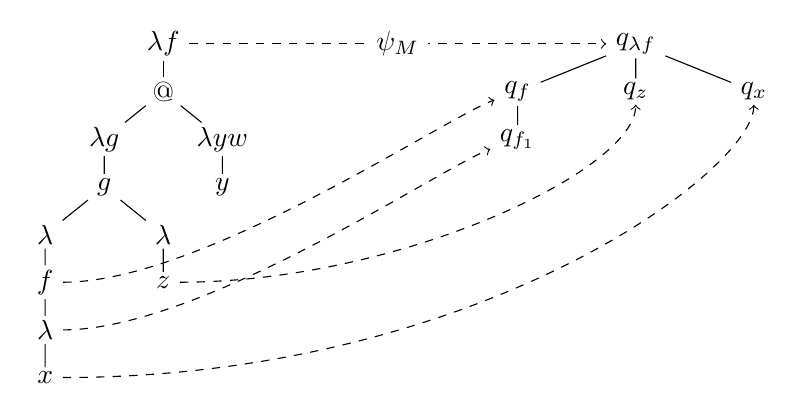
\begin{tikzpicture}[baseline=(root.base),level distance=4ex,inner ysep=0.5mm,sibling distance=15mm]
\path
node (root){$\lambda f$}
child{node{$@$}
 child{node(l1){$\lambda g$}
 child{node{$g$} child{node{$\lambda$} child{node(f){$f$}child{node(l){$\lambda$}child{node(x){$x$}}}}}
 child{node{$\lambda$}child{node(z){$z$}}}}
 }
 child{node{$\lambda y w$} child{node{$y$}}}
}
+(6cm,0)
node (qlf){$q_{\lambda f}$}
child{node(qf){$q_f$} child{node(qf1){$q_{f_1}$}}}
child{node(qz){$q_z$}}
child{node(qx){$q_x$}};
\draw[dashed,->] (root) -- node[fill=white]{$\psi_M$} (qlf);
\draw[dashed,->] (f) .. controls +(0:2cm) and +(200:1cm) .. (qf);
\draw[dashed,->] (l) .. controls +(0:2cm) and +(200:1cm) ..  (qf1);
\draw[dashed,->] (x) .. controls +(0:5.5cm) and +(-90:1cm) .. (qx);
\draw[dashed,->] (z) .. controls +(0:3cm) and +(-90:1cm) ..  (qz);
\end{tikzpicture}
\end{center}
\end{compactitem}
\end{example}

\begin{property} \
\label{proper:psi_properties}
\begin{enumerate}[(i)]
\item $\psi_M$ maps $\lambda$-nodes to O-questions, variable nodes to
P-questions, value-leaves of $\lambda$-nodes to P-answers and
value-leaves of variable nodes to O-answers;

\item $\psi_M$ preserves hereditary enabling: a node $n \in V^{\theroot\vdash}$ is hereditarily
 enabled by some node $n' \in V^{\theroot\vdash}$ in $\tau(M)$ if and only if
the move $\psi_M(n)$ is hereditarily enabled by $\psi_M(n')$ in $\sem{\Gamma \gamear T}$;

\item $\psi_M$ maps a node of a given order to a move of the same order;

\item Let $s \in \travset(M)^{\filter \theroot}$. The P-view (resp. O-view) of $\psi_M(s)$ and $s$ are computed
identically {\it i.e.}~the set of occurrence positions that must be removed
from each sequences in order to obtain their respective P-view (resp. O-view) is the same for both sequence.
\end{enumerate}
\end{property}
\begin{proof}
(i), (ii) and (iii) are direct consequences of the definition.

(iv) Because of (i) and since $t$ and $\psi_M(t)$ have the
same pointers, the computations of the P-view (resp. O-view) of the
sequence of moves and the P-view (resp. O-view) of the sequence of
nodes follow the same steps.
\end{proof}
The convention chosen to define the order of the root node (see Def.\ \ref{def:nodeorder}) permits us to have property (iii).
This explains why the order of the root node and other lambda nodes were defined differently.
\smallskip

By extension, we can define the function $\psi_M$ on $\travset(M)^{\filter \theroot}$, the set of traversal reductions, as follows:
\begin{definition}[Mapping sequences of nodes to sequences of moves]
The function $\psi_M$ maps
any traversal reduction $u = u_0 u_1 \ldots \in \travset(M)^{\filter \theroot}$ to
the following justified sequence of moves of the arena $\sem{\Gamma \gamear T}$: $\psi_M(u) = \psi_M(u_0)\ \psi_M(u_1)\  \psi_M(u_2) \ldots$ where $\psi_M(u)$ is equipped with $u$'s pointers.

The pointer-free function underlying $\psi_M$ is thus a monoid homomorphism.
\end{definition}



\subsection{Mapping traversals to interaction plays}

    Let $I$ be the interaction game of the revealed strategy $\syntrevsem{\Gamma \vdash M : T}$ and
    $M_I$ be the set of equivalence class of moves from $\mathcal{M}_I$.

    Let $r'$ be a lambda node in $N_{\sf spawn}$. We write $\Gamma(r') \vdash \kappa(r') : T(r')$ to denote the subterm of $\elnf{M}$ rooted at $r'$ (thus $\Gamma(r')\subseteq \Gamma$).
    We consider the function $\psi_{\kappa(r')}$ which maps nodes of $V^{r'\vdash}$
    to moves of $\sem{\Gamma(r') \gamear T(r')}$. Since $\mathcal{M}_I$ contains the
    moves from the standard game $\sem{\Gamma(r') \gamear A(r')}$, we can consider $\psi_{\kappa(r')}$ as a function from $V^{r'\vdash}$ to $\mathcal{M}_I$.

    Every node in $n \in V\setminus (V_@ \union V_\Sigma)$ is either hereditarily enabled by the root or by some $\lambda$-node in $N_{\sf spawn}$ (the children nodes of @/$\Sigma$-nodes). Therefore we can define the following relation $\psi^*_M$ from
    $V\setminus (V_@ \union V_\Sigma)$ to $\mathcal{M}_I$:
    $$ \psi^*_M = \psi_{M} \quad \union \Union_{r' \in N_{\sf spawn}} \psi_{\kappa(r')} \ .$$
    This relation is totally defined on $V\setminus (V_@ \union V_\Sigma)$ since those nodes are either hereditarily justified by the root, by an @-node or by a $\Sigma$-node. Moreover it is a relation and \emph{not} a function since for a given variable node $x$,
for every spawn node $r'$ occurring in the path from $x$ to $\theroot$, $x$ is hereditarily enabled by $r'$ \emph{with respect to the computation tree $\tau(\kappa(r'))$}. Thus the domains of definition of the relations $\psi_{\kappa(r')}$ for such nodes $r'$ overlap.    It can be easily check, however, that for any node $n \in V\setminus (V_@ \union V_\Sigma)$,
    the moves in $\psi^*_M (n)$ are all $\sim$-equivalent, which leads us to the following definition:

\begin{definition}[Mapping from nodes to moves of the syntactically-revealed semantics]
    \label{def:phi mapping}
    We define the \emph{function}
    $\varphi_M:V\setminus (V_@ \union V_\Sigma) \rightarrow M_I$ as follows: for $n \in V\setminus (V_@ \union V_\Sigma)$,     $\varphi_M(n)$ is defined as the $\sim$-equivalence class containing the set $\psi^*_M (n)$. We omit the subscript in $\varphi_M$ if there is no ambiguity.
\end{definition}

\begin{definition}[Mapping sequences of nodes to sequences of moves]
\label{dfn:phi_for_justsequ} We define the function $\varphi_M$ from
$\travset(M)^\star$ to justified sequence of moves in $M_I$
as follows. If $u = u_0 u_1 \ldots \in \travset(M)^\star$ then:
$$\varphi_M(s) = \varphi_M(u_0)\ \varphi_M(u_1)\  \varphi_M(u_2) \ldots$$
where $\varphi_M(u)$ is equipped with $u$'s pointers.
\end{definition}

\begin{example}
Take $M = \lambda x^o . (\lambda g^{(o,o)} . g x z) (\lambda y^o .
y)$. The diagram below represents the computation tree (middle) and
the relation $\psi^*_M = \psi_{\lambda x}\union \psi_{\lambda g. g x}
\union \psi_{\lambda y.y}$ (dashed-lines).
\begin{center}
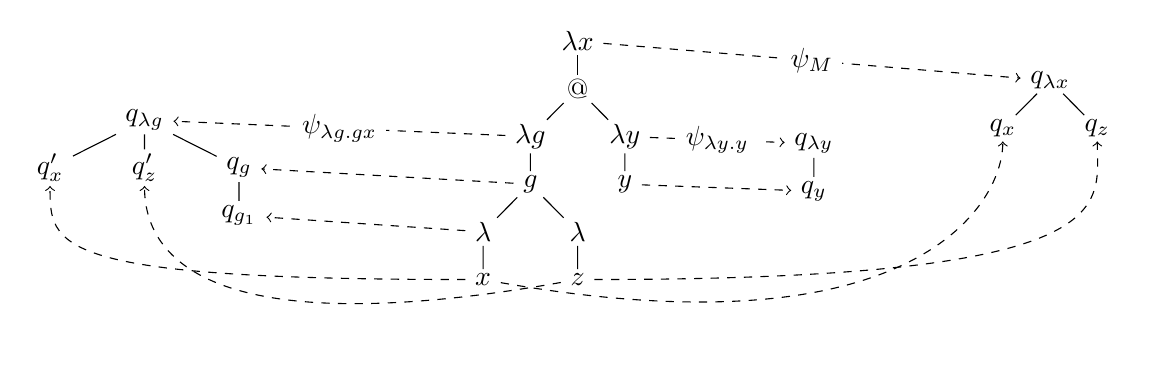
\begin{tikzpicture}[baseline=(root.base),level distance=4ex,inner ysep=0.5mm,sibling distance=12mm]
\path
node (root){$\lambda x$}
child{node{$@$}
 child{node(lg){$\lambda g$}
 child{node(g){$g$} child{node(l1){$\lambda$} child{node(x){$x$}}}
 child{node{$\lambda$}child{node(z){$z$}}}}}
 child{node(ly){$\lambda y$} child{node(y){$y$}}}}
+(6cm,-0.5)
node (qlx){$q_{\lambda x}$}
child{node(qx){$q_x$}}
child{node(qz){$q_z$}}
+(3cm,-1.3cm)
node (qly){$q_{\lambda y}$}
child{node(qy){$q_y$}}
+(-5.5cm,-1cm)
node (qlg){$q_{\lambda g}$}
child{node(qpx){$q'_x$}}
child{node(qpz){$q'_z$}}
child{node(qg){$q_g$} child{node(qg1){$q_{g_1}$}}};
\draw[dashed,->] (root) -- node[fill=white]{$\psi_M$} (qlx);
\draw[dashed,->] (x) .. controls +(-10:5.5cm) and +(-90:1cm) .. (qx);
\draw[dashed,->] (z) .. controls +(0:7cm) and +(-90:1cm) ..  (qz);
\draw[dashed,->] (ly) -- node[fill=white]{$\psi_{\lambda y.y}$} (qly);
\draw[dashed,->] (y) -- (qy);
\draw[dashed,->] (lg) -- node[fill=white]{$\psi_{\lambda g.gx}$} (qlg);
\draw[dashed,->] (g) -- (qg);
\draw[dashed,->] (l1) -- (qg1);
\draw[dashed,->] (x) .. controls +(180:5.5cm) and +(-90:1cm) .. (qpx);
\draw[dashed,->] (z) .. controls +(190:5cm) and +(-90:1cm) ..  (qpz);
\end{tikzpicture}
\end{center}
where $q_x'\sim q_x$, $q_z'\sim q_z$, $q_g\sim q_{\lambda y}$,
$q_{g_1}\sim q_y$ and $q_{\lambda g}\sim q_{\lambda x}$.
\end{example}

\begin{lemma}[Traversal projection lemma]
\label{lem:varphi_proj} Let $\odot$ denote a lambda node in $N_\lambda$, $\Delta \vdash
M^{(\odot)} : A$ be the subterm of $\elnf{M}$ rooted at $\odot$,
$t\in\travset(M)$, $r_0$ be an occurrence of $\odot$ in $t$ and $m_0$ be the occurrence of the initial $A$-move $\varphi_M(r_0)$ in
$\varphi_M(t^\star)$ then:
$$\begin{array}{rrcl}
(i)& \varphi_{M^{(\odot)}}(t^\star \filter V^{(\odot)} \filter r_0) &=& \varphi_M(t^\star) \filter \revsem{\Delta \vdash A} \filter m_0 \\ \\
(ii) & \varphi_M(\travset(M)^\star) \filter \sem{\Gamma \gamear T} &=& \psi_M(\travset(M)^{\filter \theroot})
\end{array}
$$
where $\revsem{\Delta \vdash A }$ is the interaction game of the interaction strategy denoting the subterm $M^{(\odot)}$.
\end{lemma}
\proof ($i$) Firstly we observe that the expression ``$\varphi_{M^{(\odot)}}(t^\star \filter V^{(\odot)} \filter r_0)$'' is well-defined. Indeed, by Proposition \ref{prop:trav_projection} $t\filterplus r_0$ is a traversal of $\travset(M^{(\odot)})$ therefore
the sequence $t^\star \filter V^{(\odot)} \filter r_0$, which is equal to $(t\filterplus r_0)^\star$ by Lemma \ref{lem:tstarproj_eq_tprojplusstar},
does belong to $\travset(M^{(\odot)})^\star$.

We now make the assumption that $\odot$ is a level-$2$ lambda nodes ({\it i.e.}\ a grand-child of the root $\theroot$). The proof can easily
be generalized to any lambda node by iterating the argument at every lambda nodes occurring in the path from $\odot$ to the root $\theroot$.


\emph{Claim:} The justification pointers in the sequences of nodes $t^\star \filter V^{(\odot)}$ are the same as those
of the sequence of moves $\varphi_M(t^\star) \filter \revsem{\Delta \vdash A }$.

By Definition \ref{dfn:phi_for_justsequ}, the sequences $\varphi_M(t^\star)$ and $t^\star$ have the same justification pointers,
The projection operations $\_ \filter V^{(\odot)}$ (Definition \ref{def:subterm_trav_projection})
and $\_ \filter \revsem{\Delta \vdash A}$ (Definition \ref{def:sub_interstrat_projection}) may alter the
pointers in the sequences $\varphi_M(t^\star)$ and $t^\star$, but fortunately they do so identically!
Indeed, the operation $\_ \filter V^{(\odot)}$ changes pointers only for variable nodes that are free in $V^{(\odot)}$: it makes them point to
the only occurrence of $\odot$ in the P-view at that point (which is also the only occurrence of a level-2 lambda node in the P-view).
Similarly, the operation $\_ \filter \revsem{\Delta \vdash A}$ changes pointers only for initial A-moves: it makes them point to
the only occurrence of an initial B-move in  the P-view at that point.
But free variables in $V^{(\odot)}$ are precisely mapped by $\varphi_M$ to initial A-moves and level-2 lambda nodes are mapped to
initial B-moves. Hence the claim holds.

Since the sequences $t^\star \filter V^{(\odot)}$ and  $\varphi_M(t^\star) \filter \revsem{\Delta \vdash A }$ have the same justification pointers,
the hereditary projections $\_ \filter r_0$ and $\_ \filter  m_0$ preserve exactly the same occurrence positions, thus we have
$\varphi_{M}(t^\star \filter V^{(\odot)} \filter r_0) = \varphi_M(t^\star) \filter \revsem{\Delta \vdash A} \filter m_0$.
Finally, because the function $\varphi$ is defined inductively on the structure of the computation tree we have that $\varphi_{M^{(\odot)}}$ coincides with the restriction of $\varphi_{M}$ to $M^{(\odot)}$.


($ii$) Let $H$ be the set of nodes of $\tau(M)$ which are mapped by
$\psi^*(M)$ to moves that are $\sim$-equivalent to moves in
$\sem{\Gamma \gamear T}$. We need to show that $H = V^{\theroot\vdash}$.

Since $\psi_M \subseteq \psi^*(M)$ and the image of $\psi(M)$ is
$\sem{\Gamma \gamear T}$, $H$ must contain the domain of
$\psi(M)$ which is $V^{\theroot\vdash}$.

Conversely, suppose that a node $n \in V\setminus (V_@\union V_\Sigma)$ is mapped by
$\varphi^*(M)$ to some move $m\in \mathcal{M}_I$ which is $\sim$-equivalent
to some move in $\sem{\Gamma \gamear T}$.
 If $m = \psi_M(n)$ then $n\in V^{\theroot\vdash}$. Otherwise,
$m = \psi_{\kappa(\odot)}(n)$ for some $\odot \in N_{\sf spawn}$. There
may be several node $\odot$ such that $n$ belongs to the domain of
definition of $\psi_{\kappa(\odot)}$. W.l.o.g.\ we can take $\odot$ to be
the one which is closest to the root $r$. Let $\Gamma(\odot) \vdash
\kappa(\odot) : T(\odot)$.
    \begin{compactitem}
    \item Suppose that $m$ is $\sim$-equivalent to a move in the subgame $\sem{\Gamma}$ of $\sem{\Gamma \gamear T}$
    then this means that $n$ is hereditarily justified by a free variable node in $M$ and therefore $n \in V^{\theroot\vdash}$.

    \item Suppose that $m$ is $\sim$-equivalent to a move in the subgame $\sem{T}$ of $\sem{\Gamma \gamear T}$
    then $m$ necessarily belongs to the subgame $\Gamma(\odot)$ of $\sem{\Gamma(\odot)\gamear T(\odot)}$ .
    Indeed, since $\odot$'s parent node is an application node, moves in the subgame
    $\sem{T(\odot)}$ correspond to internal moves of the application. By definition of
    the interaction strategy for the application case, such moves can only be $\sim$-equivalent to other internal
    moves and thus cannot be equivalent to move in $\sem{T}$.

    Consequently, $n$ is her.\ just.\ by a free variable node $z$ in $\kappa(\odot)$. By assumption, $\odot$ is the closest node to the root $r$ (excluding $r$ itself) for which $n$ belongs to $V^{\odot\vdash}$ (the domain of definition of $\psi_{\kappa(\odot)}$). Hence $z$ is not bound by any $\lambda$-node occurring in the path to the root. Thus $z\in
    V^{\theroot\vdash}$ and therefore $n \in V^{\theroot\vdash}$.
    \end{compactitem}
Hence $H = V^{\theroot\vdash}$. Consequently, for any traversal $t$
of $M$ we have $\varphi_M(t^\star) \filter \sem{\Gamma \gamear T} = \varphi_M(t^\star\filter V^{\theroot\vdash})$ which is equal to
$ \varphi_M(t\filter r)$ by Lemma
\ref{lem:he_proj_root_is_hj_proj_r}. \qed


\subsection{The correspondence theorem for the pure simply-typed lambda-calculus}
In this section, we establish a connection between the interaction
semantics of a pure simply-typed term (\ie without constants interpreted constants, $\Sigma = \emptyset$) and the traversals of its computation tree: we show that
the set $\travset(M)$ of traversals of the computation tree is
isomorphic to the set of uncovered plays of the strategy denotation
(this is the counterpart of the ``Path-Traversal Correspondence'' of
\cite{OngLics2006}), and that the set of traversal reductions is
isomorphic to the strategy denotation.


\emph{Notation:} For any node occurrence $n$ in a justified sequence
(of nodes or of moves) $u$ we write $\ptrdist_u(n)$, or just
$\ptrdist(n)$ if there is no ambiguity, to denote the distance
between $n$ and its justifier in $u$ if it has one, and $0$
otherwise.

\begin{lemma}[Preleminary lemma]
\label{lem:varphiinjective:prelem}
\begin{equation*}
\left(
  \begin{array}{ll}
    t \cdot n_1, t \cdot n_2 \in \travset(M) \\
    \zand\ n_1 \neq n_2
  \end{array}
\right)
 \mbox{ implies } n_1,n_2 \in V^{\theroot\vdash}_{\lambda} \zand ( \psi(n_1) \neq \psi(n_2) \zor \ptrdist(n_1) \neq \ptrdist(n_2) ) \ .
 \end{equation*}
\end{lemma}
\proof Take $t \cdot n_1, t \cdot n_2 \in \travset(M)$. Suppose that
$n_1$ and $n_2$ belong to two distinct categories of node ($N_{\sf
var}$, $N_@$, $N_\lambda$, $N_\Sigma$, $L_{\sf var}$, $L_@$, or $L_\lambda$, $L_\Sigma$)
then necessarily one must be visited with the rule
\rulenamet{InputVar} and the other by \rulenamet{InputVal} (they are
the only rules that have a common domain of definition), thus one is
a leaf-node and the other is an inner node which implies that
$\psi(n_1) \neq \psi(n_2)$.

Otherwise $n_1$ and $n_2$ belong to the same category of nodes and we proceed by case analysis:
\begin{compactitem}
\item If $n_1, n_2 \in N_@$ then $t
\cdot n_1$ and $t \cdot n_2$ are formed using the \rulenamet{App}
rule. Since this rule is deterministic we must have $n_1=n_2$ which
violates the second hypothesis.

\item If $n_1, n_2 \in L_@$ then the traversals are formed using the deterministic rule
\rulenamet{Value^{@\mapsto\lambda}} which again violates the
second hypothesis.

\item If $n_1, n_2 \in N_\Sigma$ then they are formed using a deterministic constant rule (see Def.\ \ref{def:constant_traversal}).

\item If $n_1, n_2 \in L_\Sigma$  then they are formed using a deterministic value-constant rule.

\item If $n_1,n_2\in N_{\sf var}$ then
     $t \cdot n_1$ and $t \cdot n_2$ were formed using either rule \rulenamet{Lam} or \rulenamet{App}.
     But these two rules are deterministic and their domains of definition are disjoint. Hence again the second
     hypothesis is violated.

\item If  $n_1, n_2 \in L_{\sf var}$ then either the traversals were both formed using the deterministic rule
\rulenamet{Value^{{\sf var}\mapsto\lambda}} in which case the
second hypothesis is violated; or they were formed with
\rulenamet{InputValue} in which case $n_1$ and $n_2$ are two
different value leaves belonging to $V^{\theroot\vdash}_\lambda$ and
justified by the same input variable node. Thus by definition of
$\psi$, $\psi(n_1)\neq\psi(n_2)$.

\item If  $n_1,n_2\in N_\lambda$ then the traversals $t \cdot n_1$
    and $t \cdot n_2$ must have been formed using either rule
    \rulenamet{Root}, \rulenamet{App}, \rulenamet{Var} or \rulenamet{InputVar}. Since all these rules have
    disjoint domains of definition, the same rule must have been use to
    form $t \cdot n_1$ and $t \cdot n_2$.
    But since the rules \rulenamet{Root}, \rulenamet{App} and \rulenamet{Var} are all deterministic,
    the rule used is necessarily \rulenamet{InputVar}.

    By definition of \rulenamet{InputVar}, $n_1,n_2\in N_\lambda^{\theroot\vdash}$ and the parent node of $n_1$ and the parent node of $n_2$  occur in  $\oview{t_{\prefixof x}}$ where $x \in N^{\theroot\vdash}_{\sf var}$
    denotes the pending node at $t$. If $n_1$ and $n_2$ have the same
    parent node in $\tau(M)$ then since $n_1\neq n_2$, by definition of
    $\psi$, $\psi(n_1)\neq \psi(n_2)$. If their parent node is
    different, then $n_1$ and $n_2$ are necessarily justified by two different
    occurrences in $t$ therefore $\ptrdist(n_1) \neq \ptrdist(n_2)$.

\item If  $n_1,n_2\in L_\lambda$ then either the traversals $t \cdot n_1$
    and $t \cdot n_2$ were formed using
    \rulenamet{Value^{\lambda\mapsto{\sf var}}} or they were formed with
    \rulenamet{Value^{\lambda\mapsto @}} but this is impossible since these two rules are
    deterministic and $n_1 \neq n_2$. \qed
\end{compactitem}
%end of proof




The function $\varphi_M$ regarded as a function from the set of
vertices $V \setminus V_@$ of the computation tree to moves in
arenas is not injective. (For instance the two occurrences of $x$ in
the computation tree of $\lambda f x. f x x$ are mapped to the same
question move.) However the function $\varphi_M$ defined on the set
of @-free traversals is injective, and similarly the function
$\psi_M$ defined on the set of traversal reduction is injective:

\begin{lemma}[$\psi_M$ and $\varphi_M$ are injective]
\label{lem:varphiinjective}
For any two traversals $t_1$ and $t_2$:
\begin{itemize}
\item[(i)] If $\varphi (t_1^\star) = \varphi (t_2^\star)$ then $t_1^\star =t_2^\star$\ ;
\item[(ii)] if $\psi (t_1 \filter \theroot ) = \psi (t_2 \filter \theroot )$ then $t_1\filter \theroot = t_2\filter \theroot$\ .
\end{itemize}
\end{lemma}
\proof \noindent (i) The result is trivial if either $t_1$ or $t_2$
is empty. Otherwise, suppose that $t_1^\star\neq t_2^\star$ then
necessarily $t_1 \neq t_2$. W.l.o.g.\ we can assume that the two
traversals differ only by their last node (or last node's pointer).
Thus we have $t_1 = t \cdot n_1$ and $t_2 = t \cdot n_2$ for some
sequence $t$ and some occurrences $n_1, n_2$ where either $n_1$ and
$n_2$ are two distinct node in the computation tree or
$\ptrdist(n_1) \neq \ptrdist(n_2)$.

If $n_1 = n_2$ and $\ptrdist(n_1) \neq \ptrdist(n_2)$ then $n_1,n_2$
are not @-nodes nor $\Sigma$-nodes (since for such nodes we would
have $\ptrdist(n_1) = 0 = \ptrdist(n_2)$). By definition of the
sequence $\varphi(t_1)$ we have $\ptrdist(\varphi(n_1)) =
\ptrdist(n_1)$ and similarly $\ptrdist(\varphi(n_2)) =
\ptrdist(n_2)$ thus $\varphi(t' \cdot n_1) \neq \varphi(t' \cdot
n_2)$. Finally since $n_1,n_2 \not\in (N_@ \union N_\Sigma)$ we also
have $\varphi((t' \cdot n_1)^\star) \neq \varphi((t' \cdot
n_2)^\star)$. Hence $\varphi(t_1^\star) \neq \varphi(t_2^\star)$.

If $n_1 \neq n_2$ then by Lemma \ref{lem:varphiinjective:prelem}
$n_1,n_2$ are not @-nodes or $\Sigma$-nodes (since such nodes are
not her.\ just.\ by the root) and we have either $\ptrdist(n_1) \neq
\ptrdist(n_2)$ or $\varphi(n_1) = \psi(n_1) \neq \psi(n_2) =
\varphi(n_2)$. Clearly both cases imply $\varphi(t_1^\star) \neq
\varphi(t_2^\star)$.
\smallskip

\noindent (ii) Suppose that $t_1 \filter \theroot \neq t_2 \filter \theroot$ then
necessarily $t_1 \neq t_2$. W.l.o.g.\ we can assume that the two
sequences differ only by their last occurrence. Hence we have $t_1 =
t \cdot n_1$, $t_2 = t' \cdot n_2$ for some sequence $t$ and some
nodes $n_1, n_2$ where either $n_1\neq n_2$ or $\ptrdist(n_1) \neq
\ptrdist(n_2)$.

If $n_1 \neq n_2$ then Lemma \ref{lem:varphiinjective:prelem} gives
$\psi( t_1\filter \theroot ) \neq \psi( t_2\filter \theroot )$.

If $n_1 = n_2$ then $\ptrdist(n_1) \neq \ptrdist(n_2)$.
\rulenamet{InputVar} and \rulenamet{InputValue} are the only rules
that can visit the same node with two different pointers, thus $n_1$
and $n_2$ must be in $V_\lambda^{\theroot\vdash}$. Hence:
\begin{equation*}
\psi(t_i\filter \theroot) = \psi(t\filter \theroot) \cdot \psi(n_i) \mbox{ for $i
\in \{1..2\}$}
\end{equation*}
where $\ptrdist_{\psi(t_i\filter r)}(\psi(n_i)) =
\ptrdist_{t_i\filter r}(n_i)$.

Furthermore, since $\ptrdist(n_1) \neq \ptrdist(n_2)$ and
${t_1}_{<n_1} = {t_2}_{<n_2}$ we have $\ptrdist_{t_1\filter \theroot}(n_1)
\neq \ptrdist_{t_2\filter \theroot}(n_2)$. Thus $\psi(t_1\filter \theroot) \neq
\psi(t_2\filter \theroot)$. \qed
%end of proof


\begin{corollary} \hfill
\label{cor:varphi_bij}
\begin{itemize}
\item[(i)] $\varphi$ defines a bijection from $\travset(M)^\star$
to $\varphi(\travset(M)^\star)$\ ;
\item[(ii)] $\psi$ defines a bijection from $\travset(M)^{\filter \theroot}$ to
$\psi(\travset(M)^{\filter \theroot})$\ .
\end{itemize}
\end{corollary}

\subsubsection{The correspondence theorem}
We now state and prove the correspondence theorem for the
simply-typed $\lambda$-calculus without interpreted constants
($\Sigma = \emptyset$). The result extends immediately to the
simply-typed $\lambda$-calculus with \emph{uninterpreted} constants
since we can regard constants as being free variables.


The following preliminary lemma says that extending a traversal locally also extends the
traversal globally: the traversal $t$ of $M$ can be extended by
extending a sub-traversal $t'$ of some subterm of $M$. This is
not obvious since $t'$ is a subsequence of $t$ which means that the
nodes in $t'$ are also present in $t$ with the same pointers but
with some other nodes interleaved in between. However these
interleaved nodes are inserted in a preservative way which allows us
to apply on $t$ the rule that was used to extend sub-traversal $t'$:
\begin{lemma}[Sub-traversal progression]
\label{lem:subtraversal_progression} Let $\theroot_j$ be a lambda node in $\tau(M)$,
$t$ be a justified sequence of nodes of $\tau(M)$, and $r_j$ be an occurrence of $\theroot_j$ in $t$ different from $t^\omega$.
Suppose that $\ip(t)$ is a traversal of $\tau(M)$ and $t^\omega$ appears in $t\filterplus r_j$.

If $t \filterplus r_j$ is a traversal of $\tau(M^{(\theroot_j)})$
and its last node is visited using a rule different from \rulenamet{InputVar} and $\rulename{InputVar^{val}}$
then $t$ is a traversal of $\tau(M)$.
\end{lemma}
\proof Let $t_j = t \filterplus r_j$. Since $\ip(t)$ is a traversal of
$M$, by Prop.\ \ref{prop:trav_projection} $\ip(t_j) = \ip(t)
\filterplus r_j$ is a traversal of $\tau(M^{(\theroot_j)})$.
  We proceed by case analysis on the last rule used to produce the traversal $t_j$ and we show that $t$ is a traversal of $M$:
  \begin{itemize}
    \item \rulenamet{Empty}, \rulenamet{Root}. These cases do not occur since $|t_j| \geq 2$. Indeed, $t_j$ contains at least $t^\omega$ and $r_j$ which are two different occurrences.

    \item \rulenamet{Lam}
        We have  $t_j = \ldots \cdot \lambda \overline{\xi} \cdot n$.

        Since $t_j \subseqof t$, the node $\lambda \overline{\xi}$ also occurs in $t$.
        Therefore using the rule \rulenamet{Lam} in $M$ we can form the traversal
        $t_{\prefixof \lambda \overline{\xi}} \cdot n$. But then we have $(t_{\prefixof \lambda \overline{\xi}} \cdot n) \filterplus r_j =
        t_{\prefixof \lambda \overline{\xi}} \filterplus r_j \cdot n
        = {t_j}_{\prefixof \lambda \overline{\xi}} \cdot n = t_j = t \filterplus r_j$.
        Thus, since $t$'s last node and $n$ both appear in $t\filterplus r_j$, this implies that
         $t_{\prefixof \lambda \overline{\xi}} \cdot n = t$.
        Hence $t$ is a traversal of $M$.

    \item \rulenamet{App} $t_j = \ldots \cdot \lambda \overline{\xi} \cdot @ \cdot n$.
    The same reasoning as in the previous case permits to conclude.


    \item \rulenamet{Value^{@\mapsto\lambda}} \Pstr[0.5cm]{t_j = \ldots \cdot (lmd){\lambda
        \overline{\xi}} \cdot (x){@}  \ldots  (xv-x,50:v){v}_@  \cdot
        (lmdv-lmd,30:v){v}_{\lambda \overline{\xi}} }.

    Since $t_j\subseqof t$, the nodes
    $\lambda \overline{\xi}$, $@$, $v_@$ and $v_{\lambda \overline{\xi}}$
    all appear in $t$. Moreover, since $\lambda \overline{\xi}$ is lambda node
    appearing in $t\filterplus r_j$, its immediate successor must also appear in
    $t\filterplus r_j$. Thus the two nodes $\lambda \overline{\xi}$ and $@$ are also consecutive in $t$. Hence
    we can use the rule \rulenamet{Value^{@\mapsto\lambda}} in the computation tree $\tau(M)$ to produce
    the traversal $t_{\prefixof v_{\lambda \overline{\xi}}} \cdot n$ and by the same reasoning as in the previous case, we
    conclude that necessarily $t = t_{\prefixof v_{\lambda \overline{\xi}}} \cdot n$.

    \item \rulenamet{Value^{{\sf var}\mapsto\lambda}} \Pstr[0.5cm]{t_j = \ldots \cdot (lmd){\lambda
    \overline{\xi}} \cdot (x){x}  \ldots  (xv-x,50:v){v}_x  \cdot
    (lmdv-lmd,30:v){v}_{\lambda \overline{\xi}} }. This case is identical to the previous case.

    \item \rulenamet{Value^{\lambda\mapsto @}}
          \Pstr[0.5cm]{t_j = \ldots \cdot (app){@} \cdot
        (lz-app,60){\lambda \overline{z}} \ldots
        (lzv-lz,60:v){v}_{\lambda \overline{z}} \cdot
        (appv-app,45:v){v}_@}. Same as in the previous case by observing that @ and $\lambda \overline{z}$
are necessarily consecutive in $t$.

    \item \rulenamet{InputValue} and \rulenamet{InputVar}. By assumption these cases do not happen.

    \item \rulenamet{Var}
    \Pstr[0.6cm]{ t_j = \ldots \cdot (p){p} \cdot (lx){\lambda
        \overline{x}} \ldots (x-lx,30:i){x_i}  \cdot
        (letai-p,40:i){\lambda \overline{\eta_i}} } for some
        variable $x_i \in N_{\sf var}^{@\vdash}$.

In general, two nodes $p$ and $\lambda \overline{x}$ appearing consecutively in $t_j$ are not necessarily consecutive in $t$. For in $M$, $t$ can ``jump'' from $p$ to a node that do not belong to the subterm $M^{(\theroot_j)}$, and thus not appearing in $t_j = t\filterplus r_j$.
This situation cannot happen here, however. Indeed, suppose that $t_{\prefixof p}$ extends to $t_{\prefixof p} \cdot m$ in $\tau(M)$.
 All the nodes in the thread of $\lambda \overline{\eta_i}$, in
$t_j$, are her.\ just.\ by the same initial @-node $\alpha$
which necessarily occurs after $r_j$ (the first node of $t_j$).
Consequently $p$ belongs to $N_{\sf var}^{@\vdash}$ and
therefore the traversal $t_{\prefixof p}\cdot m$ must have been
formed using the rule \rulenamet{Var} in $\tau(M)$. Since $p$
appears in $t\filterplus r_j$, by Lemma
\ref{lem:thread_projplus}(i), all the nodes in the thread of $p$
in $t$ appear in $t\filterplus r_j$. Thus $m$ appears in
$t\filterplus r_j$ (since by O-visibility it points in the
thread of $p$). Hence $(t_{\prefixof p} \cdot m)\filterplus r_0
=  t_{<p}\filterplus r_0 \cdot p \cdot m$ which implies that $m$
is precisely the occurrence $\lambda \overline{x}$.

Hence the nodes $p$, $\lambda \overline{x}$, $x_i$ and $\lambda \overline{\eta_i}$ all appear in $t$
with the two nodes $p$ and $\lambda \overline{x}$ appearing consecutively. We can therefore use the rule \rulenamet{Var} in $M$ to form the traversal $t$.

    \item \rulenamet{Value^{\lambda\mapsto{\sf var}}}. Same proof as in the previous case.
    \item \rulenamet{\Sigma}/\rulenamet{\Sigma\mbox{\sf-var}} Same as \rulenamet{App} and \rulenamet{Var}.
    \item \rulenamet{\Sigma\mbox{\sf-Value}} Same as  \rulenamet{Value^{\lambda\mapsto{\sf var}}}.
\qed
  \end{itemize}
%end of proof



The following theorem establishes a correspondence between the
game-denotation of a term and the set of traversals of its
computation tree:
\begin{theorem}[The Correspondence Theorem]
\label{thm:correspondence}
 For any simply-typed term $\Gamma \vdash M :T$,
$\varphi_M$ defines a bijection from $\travset(M)^\star$ to $\syntrevsem{\Gamma \vdash M : T}$ and $\psi_M$ defines a bijection from $\travset(M)^{\filter
\theroot}$ to $\sem{\Gamma \vdash M : T}$:
\begin{eqnarray*}
 \varphi_M  &:& \travset(\Gamma \vdash M : T)^\star \stackrel{\cong}{\longrightarrow} \syntrevsem{\Gamma \vdash M :T} \\
 \psi_M  &:& \travset(\Gamma \vdash M : T)^{\filter \theroot} \stackrel{\cong}{\longrightarrow} \sem{\Gamma \vdash M :T} \ .
\end{eqnarray*}
\end{theorem}

\begin{remark}
\label{rem:corresp_proofreduction}
    By corollary \ref{cor:varphi_bij}, we just need to show that
    $\varphi_M$ and $\psi_M$ are \emph{surjective}, that is to
    say: $\varphi_M(\travset(M)^\star) = \syntrevsem{\Gamma \vdash M : T}$
    and $\psi_M(\travset(M)^{\filter \theroot}) = \sem{\Gamma \vdash M : T}$.
    Moreover the former implies the latter, indeed:
    \begin{align*}
    \sem{\Gamma \vdash M : T} &= \syntrevsem{\Gamma \vdash M : T} \filter \sem{\Gamma \gamear T} & \mbox{by Eq.\ \ref{eqn:int_std_gamsem} from Sec.\ \ref{subsec:relating_revealed_and_standard_denotation}} \\
            &= \varphi_M(\travset(M)^\star) \filter \sem{\Gamma \gamear T} & \mbox{by assumption}\\
            &= \psi_M(\travset(M)^{\filter \theroot}) & \mbox{by lemma \ref{lem:varphi_proj}(ii)}
    \end{align*}
    therefore we just need to prove $\varphi_M(\travset(M)^\star) = \syntrevsem{\Gamma \vdash M : T}$.
\end{remark}
\smallskip

    Let us give an overview of the proof before giving it in full details.
    It proceeds by induction on the structure of the computation tree.
    The only non-trivial case is the application: the computation tree
    $\tau(M)$ has the following form:
\begin{center}
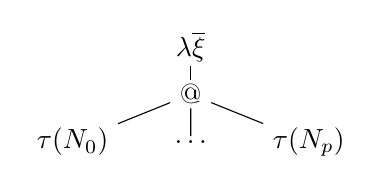
\begin{tikzpicture}[baseline=(root.base),level distance=4ex,inner ysep=0.5mm,sibling distance=15mm]
\node (root) {$\lambda\overline\xi$}
child {node {$@$}
    child{node {$\tau(N_0)$}}
    child{node{$\ldots$}}
    child{node {$\tau(N_p)$}}};
\end{tikzpicture}
\end{center}

    A traversal of $\tau(M)$ proceeds as follows: it starts at the root $\lambda \overline{\xi}$ of the tree $\tau(M)$ (rule \rulenamet{Root}), it then passes the node @ (rule \rulenamet{Lam}).
    After this initialization part, it proceeds by traversing the term $N_0$ (rule \rulenamet{App}).
    At some point, while traversing $N_0$, some variable $y_i$ bound by the root of $N_0$ is visited. The traversal
    of $N_0$ is interrupted and jumps (rule \rulenamet{Var}) to the root of $\tau(N_i)$. The process then goes on with $\tau(N_i)$.
    When traversing $N_i$, if the traversal encounters a variable bound by the root of $\tau(N_i)$ then the traversal of $N_i$
    is interrupted and
    the traversal of $N_0$ resumes.  This schema is repeated until the traversal of $\tau(N_0)$ is completed\footnote{Since we are considering
    simply-typed terms, the traversal does indeed terminate. However this will not be true anymore in the \pcf\ case.}.

    The traversal of $M$ is therefore made of an initialization part followed by an interleaving of a traversal of $N_0$ and
    several traversals of $N_i$ for $i=1..p$. This schema is reminiscent of the way the evaluation copycat map $ev$ works in game semantics.

    The key idea is that every time the traversal pauses the traversal of a subterm and switches to another one,
    the jump is permitted by one of the ``copycat'' rules \rulenamet{Var}, \rulenamet{Value^{\lambda\mapsto @}}, \rulenamet{Value^{{\sf var}\mapsto\lambda}} or \rulenamet{Value-var}.
    We show by (a second) induction that these copycat rules define precisely what the copycat strategy $ev$ performs on sets of plays.
\smallskip

\proof
Let $\Gamma \vdash M : T$ be a simply-typed term where $\Gamma =
x_1:X_1,\ldots x_n:X_n$. We assume that $M$ is already in
$\eta$-long normal form. By remark \ref{rem:corresp_proofreduction} we just need to
show that $\varphi_M(\travset(M)^\star) = \syntrevsem{\Gamma \vdash M : T}$.
We proceed by induction on the structure of $M$:
\begin{itemize}[$\bullet$]
    \item (abstraction) $M \equiv \lambda \overline{\xi}. N : \overline{Y} \typear B$ where $\overline{\xi} = \xi_1:Y_1,\ldots \xi_n:Y_n$. On the first hand we have:
\begin{eqnarray*}
\syntrevsem{\Gamma \vdash \lambda \overline{\xi}. N:T} &=& \Lambda^n( \syntrevsem{\overline{\xi}, \Gamma \vdash N: B } ) \\
        &\simeq& \syntrevsem{\overline{\xi}, \Gamma \vdash N: B } \ .
\end{eqnarray*}
On the other hand, the computation tree $\tau(N)$ is isomorphic to
$\tau(\lambda \xi_1\ldots \xi_n . N)$ (up to a renaming of the root
of the computation tree) and $\travset(N)$ is isomorphic to
$\travset(\lambda \xi_1\ldots \xi_n . N)$.
Hence we can conclude using the induction hypothesis.

  \item (variable) $M \equiv x_i$. Since $M$ is in $\eta$-long normal form, $x$ must be of ground
      type. The computation tree $\tau(M)$ and the arena $\syntrevsem{\Gamma \gamear o}$ are represented below
      (value leaves and answer moves are not represented):
\begin{center}
\begin{tikzpicture}[baseline=(root.base),level distance=4ex,sibling distance=12mm,level 2/.style={sibling distance=8mm}]
\path node (root) {$\lambda$} child[level distance=6ex] {node {$x_i$}}
+(5cm,0)
node {$q_0$}
child {node {$q_1$}
    child[dotted]{node{}}
    child[dotted]{node{}}
    }
child {node {$q_2$}
    child[dotted]{node{}}
    child[dotted]{node{}}
    }
child{node{$\ldots$}}
child {node {$q_n$}
    child[dotted]{node{}}
    child[dotted]{node{}}
    };
\end{tikzpicture}
\end{center}
        Let $\pi_i$ denote the $i$th projection of the interaction game
        semantics. We have:
        \begin{align*}
        \syntrevsem{M} &= \pi_i = \prefset(\{ \Pstr{(q0){q_0} \cdot (qi){q^i} \cdot (vqi-qi){v_{q^i}} \cdot (vq0-q0){v_{q_0}} } \ | \ v\in \mathcal{D} \})\ .
        \end{align*}

        It is easy to see that traversals of $M$ are precisely
        the prefixes of $ \Pstr{ (lmd)\lambda \cdot (xi){x_i}
        \cdot (vxi-xi){v_{x_i}} \cdot (vlmd-lmd){v_{\lambda}}}$.
        $M$ is in $\beta$-normal therefore $\travset(M)^\star =
        \travset(M)$ and since $\varphi_M(\lambda) = q_0$ and
        $\varphi_M(x_i) = q^i$, we have:
        $$ \varphi_M(\travset(M)^\star) = \varphi_M(\travset(M)) = \varphi_M(\prefset( \lambda \cdot x_i \cdot v_{x_i} \cdot v_{\lambda}))
         = \syntrevsem{M} \ .
        $$


    \item (@-application) $M = N_0 N_1 \ldots N_p :o$ where $N_0$ is not a variable.
    We have the typing judgments $\Gamma \vdash N_0 N_1 \ldots
    N_p : o$ and $\Gamma \vdash N_i : B_i$ for $i\in 0..p$ where
    $B_0 = (B_1,\ldots,B_p,o)$ and $p\geq 1$.

    The tree $\tau(M)$ has the following form:
\begin{center}
\begin{tikzpicture}[baseline=(root.base),level distance=5ex,inner ysep=0.5mm,
sibling distance=20mm]
\node(root){$\lambda^{[\theroot]}$}
child{node{$@$}
    child{node{$\lambda y_1 \ldots y_p^{[\theroot_0]}$}
       child[child anchor=north,level distance=1ex] {node[isosceles triangle,draw,anchor=north,shape border rotate=90]{$\tau(N_0)$}}
    }
    child{node{$[\theroot_1]$}
       child[child anchor=north,level distance=1ex] {node[isosceles triangle,draw,anchor=north,shape border rotate=90]{$\tau(N_1)$}}
    }
    child{node{$\ldots$}}
    child{node{$[\theroot_p]$}
       child[child anchor=north,level distance=1ex] {node[isosceles triangle,draw,anchor=north,shape border rotate=90]{$\tau(N_p)$}}
    }
};
\end{tikzpicture}
\end{center}
    where $\theroot_j$ denote the root of $\tau(N_j)$ for $j\in
    \{0..p\}$.

    We have:
    $$
    \syntrevsem{\Gamma \vdash M : o}
            =  \underbrace{\langle \syntrevsem{\Gamma \vdash N_0 : B_0}, \ldots, \syntrevsem{\Gamma \vdash N_p : B_p} \rangle}_{\Sigma}\ \| \ ev
    $$

    We refer the reader to Figure \ref{fig:interaction_strategy_denotations} from the previous section for a tree-representation of $\syntrevsem{M}$ which fixes the names of the different games involved in the interaction strategy. In particular the games $A$, $B$ and $C$ are defined as:
    \begin{eqnarray*}
        A &=& X_1 \gameprod \ldots \gameprod X_n\\
        B &=& \underbrace{((B_1' \gameprod \ldots \gameprod B_p') \gamear o')}_{B_0} \gameprod B_1 \gameprod \ldots \gameprod B_p\\
        C &=& o \ .
    \end{eqnarray*}


    Let $q_0$ and $q_0'$ be the initial
    question of $C$ and $B_0$ respectively.

%    Since $\varphi_M = \psi_M \union \varphi_{N_0} \union
%    \varphi_{N_1}$ the induction hypothesis gives us:
%    \begin{align}
%    \varphi_{M} (\travset(N_0)^\star) &= \syntrevsem{\Gamma \vdash N_0 : B_0} \label{eqn:ih_1} \\
%    \varphi_{M}(\travset(N_1)^\star) &= \syntrevsem{\Gamma \vdash N_1 : B_1} \label{eqn:ih_2}
%    \end{align}
\begin{enumerate}
\item[$\subseteq$]
    We first prove that $\syntrevsem{\Gamma \vdash M : T}
    \subseteq \varphi_{M}( \travset(M)^\star )$. Suppose $u
    \in \syntrevsem{\Gamma \vdash M : T}$. We give a
    constructive proof that there is a traversal $t$
    such that $\varphi_M(t^\star) = u$ by induction on
    $u$.

    For the base case $u=\epsilon$, take $t$ to be the empty traversal formed with \rulenamet{Empty}.
    \emph{Step case:} Suppose that $u = u' \cdot m \in
    \syntrevsem{\Gamma \vdash M : T}$ for some move $m \in
    M_T$ where $u' = \varphi_M(t'^\star)$ for some traversal
    $t'$ of $\tau(M)$.

    By unraveling the definition of $u \in \syntrevsem{\Gamma \vdash M : T}$ we have:
    \begin{equation}
    \left\{
    \begin{array}{ll}
        u \in L_T ;  \\
        \hbox{For any occurrence $b$ in $u$ of an initial $B_k$-move, for some $k \in \{0..p\}$:} \\
        \left\{\begin{array}{ll}
            u \filter T^{0k} \filter b  \in \syntrevsem{N_k} \\
            u \filter T^{0k'} \filter b  = \epsilon \quad \mbox{ for every } k'\in \{0..p\}\setminus\{k\};
        \end{array}
        \right. \\
        u \filter B_0 = u \filter B_1, \ldots, B_p, C \ .
    \end{array}
    \right.
      \label{eqn:u_in_app_intersem}
    \end{equation}

We recall that $m \in M_T$ is an equivalence class of moves
from $\mathcal{M}_T$. For any game $A$ appearing in the
interaction game $T$ we will write ``$m \in A$'' to mean
that some citizen of the class $m$ belongs to the set of
moves $M_A$. Similarly, for any sub-interaction game $T'$ of
$T$, we write ``$m \in T'$'' to mean that some citizen of
the class $m$ belongs to the set of moves
$\mathcal{M}_{T'}$. We proceed by case analysis on $m$; we either have $m\in C$ or $m\in T^0$. In the last case $m$ is either in $A$, a superficial internal move in $B$ or a profound internal move in $B$:
    \begin{itemize}
    \item Suppose $m \in C$. Moves in $C$ are played by the standard strategy $ev$ that does not contain any internal move. Hence $m$ is either $q_0$ or $v_{q_0}$ for some $v\in\mathcal{D}$.

    Suppose that $m=q_0$. Since $q_0$ can occur only once in
    $u$ we have $u=q_0$ and the traversal $t=\lambda^{[\theroot]}$ formed with \rulenamet{Root} clearly verifies $\varphi(t^\star) = u$.

    Suppose that $m=v_{q_0}$. Since $m$ is a P-move played by the
    copy-cat strategy $ev$ in $B,C$, it must be the copy of some move $v_{q_0'}$ that answers the question $q_0'$ in the sub-game $o'$.

    In fact $v_{q_0'}$ is precisely $u'$'s last move. Indeed
    suppose that $u' = \ldots v_{q_0'} \cdot u''$. The play
    $u'_{\prefixof v_{q_0'}}\filter A,B$ is complete since its
    first move $q_0'$ is answered by $v_{q_0'}$. Therefore by
    Lemma \ref{lem:inter_complete}(ii), $u'_{\prefixof
    v_{q_0'}}\filter T^0$ is maximal. Thus moves in $u''$ must
    be played in $T^1$ by $ev$, but since $ev$ does not play internal
    moves, $u''$ is necessarily empty.

    Consequently, by the induction hypothesis, the last move in $t'$ is $\varphi(v_{q_0'}) = v_{\lambda y_1}$.
    The rules \rulenamet{Value^{\lambda\mapsto @}} and \rulenamet{Value^{@\mapsto\lambda}} permits us to extend
    the traversal $t'$ into $t' \cdot v_@ \cdot v_{\lambda \overline{\xi}}$ where $v_@$ and $v_{\lambda
    \overline{\xi}}$ point to the second and first node of $t'$ respectively. Clearly we have $\varphi_M((t'\cdot v_@ \cdot v_{\lambda \overline{\xi}})^\star) = u$.

    \item Suppose $m\in T^0$ and $m$ is an initial move in $B_0$.
    Then necessarily $m$ is $q_0' \in \sem{o'}$, the copy-cat move of the initial move $q_0 \in C$ of $u$. Hence $u = q_0 \cdot q_0'$. The rules \rulenamet{Root}, \rulenamet{App}
and \rulenamet{Lam} permit us to build the traversal $t =
\lambda^{[\theroot]} \cdot @ \cdot \lambda
\overline{y}^{[\theroot_0]}$ which clearly verifies
$\varphi_M(t^\star) = u$.

    \item Suppose $m\in T^0$ and $m$ is an initial move in $B_k$ for some $k\in \{1..p\}$.

    Then $m$ is necessarily a copy-cat move played by the evaluation strategy, and the move $m^1$ immediately preceding $m$ in $u$ is an initial move of the component $B'_k$ of $B_0$.

    Thus since $\varphi_M(t'^\omega) = m^1$, $t'^\omega$ must be an occurrence of the node $y_k$, the $k^{th}$ variable bound by $\lambda \overline{y}$. Hence using the rule \rulenamet{Var} we can form the traversal $t= t' \cdot \theroot_k$ verifying $\varphi_M(t^\star) = \varphi_M(t'^\star) \cdot m = u$.


    \item Suppose $m\in T^0$ and $m$ is not initial in $B$. In $u \filter T^0$, $m$ must be hereditarily justified by some initial move $b$ in $B_k$ for some $k\in \{0..p\}$. Since $u \filter T^{0k} \filter b \in \syntrevsem{N_k}$, the outermost induction hypothesis gives us:
        \begin{equation}
        u \filter T^{0k} \filter b = \varphi_{N_k}(t_k^\star)  \label{eqn:corresp_outmost_ih}
        \end{equation}
        for some traversal $t_k \in \travset(N_k)$ where w.l.o.g.\ we can assume that $t_k^\omega \not\in V_@$. We have:
        \begin{align*}
            \varphi_M (t_k^\omega) &= (\varphi_M (t_k^\star))^\omega & \mbox{($t_k^\omega \not\in V_@$)}\\
                                   &= ((u' \cdot m) \filter T^{0k}\filter b)^\omega & \mbox{(by Eq.\ \ref{eqn:corresp_outmost_ih})}\\
                                   &= ((u' \filter T^{0k}\filter b) \cdot m))^\omega & \mbox{($m$ is h.j. by $b$ and belongs to $T^{0k}$)}\\
                                   &= m \ .
        \end{align*}

        Take $t = t'\cdot t_k^\omega$ where $t_k^\omega$ points in $t'$ to the image by $\varphi_M$ of the occurrence justifying $m$ in $u$. Since $t_k^\omega \neq @$ we have  $t^\star = t'^\star \cdot t_k^\omega$ where $t_k^\omega$ justifier in $t'^\star$ is the same as its justifier in $t$.


        Hence we have $\varphi_{M}(t^\star) =  \varphi_{M}(t'^\star)  \cdot \varphi_{M}(t_k^\omega)$ which, by the innermost I.H.\ together with the previous equation, is equal to $u' \cdot m$ where $m$'s justifier in $u'$ corresponds to $\varphi_{M}(t_k^\omega)$'s justifier in $\varphi_{M}(t'^\star)$. Consequently:
        \begin{equation}
                \varphi_M(t^\star) =  u  \label{eqn:corresp_phi_t_minu_at_eq_u}
        \end{equation}
\smallskip

        We are half-done at this point: it remains to show that $t$ is indeed a traversal of $\tau(M)$.

        Let $r_k$ denote the occurrence of the root
        $\theroot_k$ in $t$ that is mapped to the
        occurrence $b$ in $\varphi_{M}(t^\star)$. We make the following claim:
        \begin{equation}
            t_k = t \filterplus r_k \ . \label{equ:claim_tk}
        \end{equation}

        Indeed we have:
        \begin{align*}
        \varphi_{N_k}(t_k^\star) &= u \filter T^{0k}\filter b
            & \mbox{(By Eq.\ \ref{eqn:corresp_outmost_ih})} \\
         &= \varphi_{M}(t^\star) \filter T^{0k}\filter b
            & \mbox{(By Eq.\ \ref{eqn:corresp_phi_t_minu_at_eq_u})} \\
         &= \varphi_{N_k}(t^\star \filter V^{(\theroot_k)} \filter r_k )
            & \mbox{(By Lemma \ref{lem:varphi_proj}(i)).}
        \end{align*}
        Since $\varphi_{N_k}$ is a bijection from  $\travset(N_k)^\star$ to $\varphi_{N_k}(\travset(N_k)^\star )$ (by Corollary \ref{cor:varphi_bij}) this implies that  $t_k^\star = t^\star \filter V^{(\theroot_k)} \filter r_k$ which in turn is equal to $(t\filterplus r_k)^\star$ by Lemma \ref{lem:tstarproj_eq_tprojplusstar} from Section \ref{sec:tstar}. But since $t_k$ and $t$ do not end with an @-node, this implies the equality from Equation \ref{equ:claim_tk}.
    \smallskip

    We now show that $t$ is indeed a traversal by case analysis on the rule used to visit the last occurrence of $t_k$ in the tree $\tau(N_k)$:
    \begin{enumerate}[(a)]
    \item  Suppose the rule used to visit $t_k^\omega$ is \emph{not} \rulenamet{InputVar} nor $\rulename{InputVar^{val}}$.
        Then by Lemma \ref{lem:subtraversal_progression}, $t$ is a traversal of $M$.

    \item Suppose $t_k^\omega$ is visited with \rulenamet{InputVar}. Then $t_k$ is of the form
        $$\Pstr[17pt]{ t_k = \ldots \cdot (z)z \cdot \ldots \cdot (n-z){t_k^\omega}}$$
        for some input-variable $z \in
        N^{\theroot_k\vdash}_{\sf var}$ occurring in
        $\oview{t_k}$ and where $t_k^\omega \in N_\lambda^{\theroot_k\vdash}$.


        Thus:
        $$u = \Pstr[0.5cm]{ \ldots \cdot (m3){\stk{\psi_{N_k}(z)}{=m^3}} \cdot
                    \ldots \cdot (m-m3,30){\stk{\psi_{N_k}(t_k^\omega)}{=m}} } $$


%        Since $z$ is her.\ enabled by the $\theroot_k$ and
%        appears in $\ip(t_k) = t' \filterplus r_k$, it is
%        necessarily her.\ \emph{justified} by $r_k$ in
%        $t_k$. Thus $\psi_{N_k}(z)$ is her.\ just.\ by $b \in B_k$ in $\psi_{N_k}(t_k\filter r_k)$
%        (and therefore so is $\psi_{N_k}(t_k^\omega)$).

        Since $t_k^\omega$ is her.\ enabled by the the root $\theroot_k$ which itself is enabled by an application node, it cannot be her.\ enabled by the root $\theroot$ in $M$. Therefore the move $\psi_{N_k}(t_k^\omega)$ is not played in $A$ (since only node that are her.\ enabled by the root are mapped to move in $A$). Hence $\psi_{N_k}(t_k^\omega) \in B_k$. Similarly, $\psi_{N_k}(z) \in B_k$.

        Now let us consider the top-most composition in the interaction strategy $\syntrevsem{M}$: the interaction strategy $\Sigma: A \gamear B$ get composed with the evaluation copy-cat strategy $ev:B \gamear o$. Consider $ u \filter A,B,C$ - the sub-sequence of $u$ containing only moves involved in this top-most composition ({\it i.e.}\ where the internal moves coming from other compositions at deeper level in the interaction semantics are removed). Since $z$ is a variable node, the move $m^3 = \psi_{N_k}(z) \in B_k$ is a P-move with \emph{respect to the game} $\sem{A \gamear B_k}$, and therefore it is an O-move in the game $\sem{B \gamear o}$. Consequently the strategy $ev$ is responsible to play at $u_{\prefixof m^3} \filter A, B, C$. Let us call $m^2$ the move played by $ev$ which immediately follows $m^1$ in $u\filter A,B,C$.

        We claim that $m^3$ and $m^2$ are also consecutive in $u$. That is to say that no internal moves generated from the        other compositions at deeper levels in the interaction strategy can ever be played between $m^3$ and $m^2$. Indeed, firstly the strategy $ev$ is a pure standard strategy thus it does not play any internal move. Furthermore, suppose that the strategy $\Sigma$ comes from the composition $\Sigma_l \| \Sigma_r$ of two interaction strategies $\Sigma_l: A \gamear D$ and $\Sigma_r: D\gamear B$ for some game $D$, then by the Switching Condition for function-space game (\cite{hylandong_pcf}) the Opponent cannot switch of component, and thus the move following $m^3$ in the interaction sequence $u \filter A,D,B$ must belong to $B$. Hence internal moves from $D$ cannot be played immediately after $m^3$.

        Similarly, we can show that the move $m$ is played by the strategy $ev$ and is the copy of the move $m^1$ immediately preceding it in $u\filter A,B,C$ as well as in $u$.

        Hence the sequence $u$ has the following form:
        $$u = \Pstr[0.6cm]{ \ldots \cdot (m3){m^3} \cdot
                    (m2){m^2} \cdot \ldots \cdot
                    (m1-m2,30:i){m^1} \cdot (m-m3,37:i){m} } $$
        Consequently we have:
        \begin{align*}
        t_k &= \Pstr{ \ldots \cdot (m)z \cdot \ldots \cdot (n-m,30:i){t_k^\omega} }  &
        t'&= \Pstr[0.5cm]{ \ldots \cdot z \cdot (n2){\lambda \overline{y}} \cdot \ldots \cdot (n1-n2,30:i){y} }
        \end{align*}

        The first equation implies that $t_k^\omega$ is the $i^{th}$ child of $z$ in the computation tree,
        thus since $z\not\in N^{\theroot\vdash}$, we can apply the (Var) rule to the second equation which produces the traversal of $\tau(M)$:
        \begin{eqnarray*}
            t' \cdot t_k^\omega = \Pstr[0.5cm]{ \ldots \cdot (n3){z} \cdot (n2){\lambda \overline{y}} \cdot \ldots \cdot (n1-n2,30:i){y} \cdot (n-n3,35:i){t_k^\omega} }
        \end{eqnarray*}
        which is precisely the sequence $t$. Hence $t$ is indeed a traversal of $\tau(M)$.

    The diagram on figure \ref{fig:example_seq_u} shows an example of such interaction sequence $u$.
    \begin{figure}[htbp]
    \centering
    \begin{tikzpicture}[style={anchor=base}]   
    \matrix [matrix of math nodes, column sep=1ex, row sep=0pt]
    {   & A & \longrightarrow & ( (B_1' &\gamear & o') & \gameprod & B_1 ) & \longrightarrow & o  \\
      &&& &&&&&& \node(q0){q_0 (\lambda \overline{\xi})}; & O\\
      &&& &&&&&  \\
    O &&& && \node(q1){q_0' (\lambda \overline{z})}; &&&&& P \\
    P &&& \node(m3){m^3 (z)}; &&&&&&& O \\
    O &&& &&&& \node(m2){m^2 (\lambda \overline{y})}; &&& P \\
    P &&& &&&& \node(m1){m^1 (y)}; &&& O \\
    O &&& \node(m){m (t_k^\omega)}; &&&&&&& P \\
    }; 
    \path[->,draw] (q1) -- node[fill=white]{@} (q0);
    \path[->,draw] (m1.west) .. controls +(160:7pt) and +(200:5pt) .. (m2.west);
    \path[->,draw] (m3) -- (q1);
    \path[->,draw] (m) --  (m3);
    \path[->,draw] (m2) -- (q0);
    \end{tikzpicture}
    \caption{Example of a sequence $u\filter A,B,C$ for $u\in\syntrevsem{M}$ and $l=1$.}
    \label{fig:example_seq_u}
    \end{figure}


    \item Suppose $t_k$'s last move is visited with the rule $\rulename{InputVar^{val}}$ then the proof is the same as in the previous case but with $\rulename{InputVar^{val}}$ substituted for $\rulename{InputVar}$.
    \end{enumerate}

    \end{itemize}

\item[$\supseteq$]
  The converse, $\varphi_{M}( \travset(M)^\star) \subseteq \syntrevsem{M}$, is the easy part of the proof.

  Let $u$ be as sequence of $\varphi_{M}( \travset(M)^\star)$. Then
  $u = \varphi_{M}(t^\star)$ for some traversal $t$ of $\tau(M)$. To show that
  $u$ is a position of $\syntrevsem{\Gamma \vdash M : T}$ we have to prove that it satisfies condition (\ref{eqn:u_in_app_intersem}):
\begin{itemize}
    \item $\varphi_{M}(t^\star) \in L_T$: It suffices to show that $\varphi_{M}(t^\star) \filter \sem{type(T)}$ is a legal
    standard position for any subtree $T'$ of $T$. This reduces to showing that for any lambda node $n$ in the $\tau(M)$,
    $t^\star \filter V^{(n)}$ is well-bracketed, satisfy visibility and alternation. But this follows immediately from the fact that $t$ verifies these properties (since $t$ is a traversal).

    \item Take an initial $B$-move $b \in B_k$, for some $k\in\{0..p\}$, occurring in $\varphi_{M}(t^\star)$. There is a corresponding occurrence $r_k$ in $t$ of a level-$2$ lambda node $\theroot_k$ of $\tau(M)$.

    By definition, the function $\varphi_{M}$ maps nodes from the subtree of $\tau(M)$ rooted at $\theroot_{k'}$, for any $k'\in \{0..p\}$, to moves of the game $\syntrevsem{\Gamma \vdash B_{k'}}$ that are hereditarily justified by some occurrence of $\varphi_M(\theroot_{k'})$.
    Hence for any $k'\in \{0..p\}\setminus\{k\}$ we clearly have $\varphi_{M}(t^\star) \filter T^{0k'} \filter b = \epsilon$.
    Moreover:
    \begin{align*}
        u \filter T^{0k}\filter b &= \varphi_{M}(t^\star) \filter T^{0k}\filter b \\
         &= \varphi_{M}(t^\star \filter V^{(\theroot_k)} \filter r_k ) & \mbox{by Lemma \ref{lem:varphi_proj}(i)} \\
         &= \varphi_{M}((t\filterplus r_k)^\star) & \mbox{by Lemma \ref{lem:tstarproj_eq_tprojplusstar}} \\
         &= \varphi_{N_k}((t\filterplus r_k)^\star) & \mbox{since $t\filterplus r_k$ is a traversal of $N_k$ by Prop.\ \ref{prop:trav_projection}} \\
         &\in \varphi_{N_k}(\travset(N_k)^\star) \\
         &\quad = \syntrevsem{N_k} & \mbox{by the induction hypothesis.}
    \end{align*}
    \item  Finally we can show that $\varphi_{M}(t^\star) \filter B_0 = \varphi_{M}(t^\star) \filter B_1, \ldots, B_p, C$ by a trivial induction on the traversal $t$. (This property holds thanks to the copycat traversal rules which mimic the behaviour of the evaluation strategy).
    \end{itemize}

\end{enumerate}


    \item (Var-application) $M = x_i N_1 \ldots N_p :o$.

    The revealed denotation is
    $\syntrevsem{\Gamma \vdash M : o} =  \underbrace{\langle
            \pi_i, \syntrevsem{\Gamma \vdash N_1 : B_1}, \ldots,
            \syntrevsem{\Gamma \vdash N_p : B_p} \rangle}_{\Sigma}
            ;^{\emptyset,\{1..p\}} \ ev$
    and the computation tree is
%\parpic(5.5cm,4cm)[r]
{\begin{center}
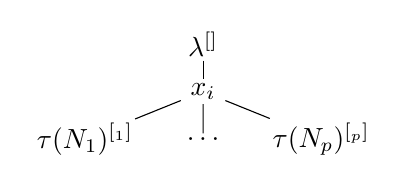
\begin{tikzpicture}[baseline=(root.base),level distance=4ex,inner ysep=0.5mm,sibling distance=15mm]
\node (root) {$\lambda^{[\theroot]}$}
child {node {$x_i$}
    child{node{$\tau(N_1)^{[\theroot_1]}$}}
    child{node{$\ldots$}}
    child{node{$\tau(N_p)^{[\theroot_p]}$}}};
\end{tikzpicture}
\end{center}
   }.

    Figure \ref{fig:interaction_strategy_denotations} from the previous section fixes the names of the different games involved in the interaction strategy.
    The composition of $\Sigma$ with $ev$ takes place on the game
    $$ \overbrace{X_1 \times \ldots \overbrace{((B_1'' \times \ldots \times B_p'') \typear o'')}^{X_i} \ldots \times X_n}^A \stackrel\Sigma\longrightarrow \overbrace{\psframebox[linestyle=dashed]{ \overbrace{((B_1' \times \ldots \times B_p') \typear o')}^{B_0} \times B_1 \times \ldots B_p }}^B \stackrel{ev}\longrightarrow \overbrace{o}^C$$

    Let $q_0$, $q_0'$ and $q_0''$ be the initial
    question of $C$, $B_0$ and $X_i$ respectively.
    \begin{description}
        \item[$\syntrevsem{\Gamma \vdash M : T} \subseteq \varphi_{M}( \travset(M)^\star )$.] We show (constructively) by induction that for any $v \in \Sigma \| ev$, there is some traversal $t$ such that
        the sequence $u = \cover(v, \{0..p\}, \{0\})$ is equal to $\varphi_M(t^\star)$.

    The base case $v=\epsilon$ is trivial. Suppose that $v = v' \cdot m \in  \Sigma   \| ev$  where $\cover(v', \{0..p\}, \{0\}) = \varphi_M(t'^\star)$ for some traversal $t'$ of $\tau(M)$ and move $m \in M_T$. Unraveling the definition of $v \in \Sigma \| ev$ gives
    \begin{equation}
    \left\{
    \begin{array}{ll}
              & v \in L_T \\
        \zand & \hbox{For any occurrence $b$ in $v$ of an initial $B_k$-move for some $k \in \{0..p\}$:} \\
        & \left\{\begin{array}{ll}
            v \filter T^{00} \filter b  \in \pi_i \hbox{ if $k=0$ and } v \filter T^{0k} \filter b  \in \syntrevsem{N_k} \hbox{ if $k>0$;} \\
            \hbox{and } \forall k'\in \{0..p\}\setminus\{k\} .\ v \filter T^{0k'} \filter b  = \epsilon
        \end{array}
        \right. \\
        \zand & v \filter B_0 = v \filter B_1, \ldots, B_p, C \ .
    \end{array}
    \right.
    \label{eqn:u_in_varapp_intersem}
    \end{equation}



    We proceed by case analysis on $m$. It is either played in $A$, $B$ or $C$.
        \begin{enumerate}[1.]
            \item $m\in C$. The proof is the same as in the @-application case except that the rules \rulenamet{Value^{\lambda\mapsto{\sf var}}} and \rulenamet{Value^{{\sf var}\mapsto\lambda}} are used instead of \rulenamet{Value^{\lambda\mapsto @}} and \rulenamet{Value^{@\mapsto\lambda}} respectively.

            \item $m$ is a superficial internal $B$-move. Then $\cover(v,\{0..p\}, \{0\}) = \cover(v', \{0..p\}, \{0\})$ so we can directly conclude from the I.H.

            \item $m$ is a profound internal $B$-move. Then necessarily $m$ belongs to $B_k$ for some $k\in \{1..p\}$ (since $\pi_i$ does not contain internal moves). Thus $m$ must be hereditarily justified by some $b \in B_k$. The treatment of this case is identical to the @-application case where $m\in T^0$ is not initial in $B$ and $b \in B_k$ for some $k\in \{0..p\}$.

            \item $m \in A$. Let $b$ denote the initial $B_k$-move that hereditarily justifies $m$ for some $k \in\{0..p\}$.
                  If $k>0$ then the treatment is the same as in case 3. Otherwise $b \in B_0$:

                   \begin{itemize}
                     \item Suppose $m$ is an occurrence of the initial $o''$-move $q_0''$. Then $m$ is played by $\pi_i$ and therefore is the copy of $q_0'$ itself the copy of the initial move $q_0$ of $v$. Thus $v = q_0 \cdot q_0' \cdot q_0''$ and $u = q_0 \cdot q_0''$. The traversal $t = \lambda^{[\theroot]} \cdot x_i$ formed using the rules \rulenamet{Root} and \rulenamet{Lam} meets the requirement.

                   \item Otherwise since $v \filter b \in \pi_i$ we have $ v \filter b \filter X_i = v \filter b \filter B_0$ therefore $m$ must necessarily be hereditarily justified by the \emph{first} occurrence of $q_0''$ in $v$.

                       \begin{itemize}
                         \item Suppose $m$ is an $\omove$-question.

                       Then the preceding move in $v$ is necessarily a $\pmove$-move also played in $A$ by the strategy $\pi_i$ and therefore it is also her.\ just.\ by the first occurrence of $q_0''$.

                       Then by definition of $\varphi_M$, the last node in  $t'$ is a variable node (if the preceding move is a $\pmove$-question) or a value-leaf of a lambda node (if the preceding move is a $\pmove$-answer) that is hereditarily justified by the node $x_i$. Hence the  rule \rulenamet{InputVar} can be applied at $t'$.

                       Let $m'$ be $m$'s justifier in $v'$ and $\alpha'$ be the corresponding node in $t'$ that $\varphi_M$ maps to $m'$.
                       Suppose $m$ is the $i$th move enabled by $m'$ in the arena, then let us write $\alpha$ be the $i$th child node of $\alpha'$ in $\tau(M)$. By definition of $\varphi_M$ we have $\varphi_M(\alpha) = m$.
                       We want to show that \rulenamet{InputVar} can extend $t'$ with $\alpha$. Since we have $v\filter A,C \in \sem{M}$, by O-visibility $m'$ appears in $\oview{v'\filter A,C}$, and by the induction hypothesis we have $v'\filter A,C = \psi_M (t'\filter r)$. Hence \begin{align*}
                       m' \in \oview{\psi_M (t'\filter r)} &= \psi_M ( \oview{t'\filter r}) \\
                          &= \varphi_M ( \oview{t' \filter r}) & \mbox{Since $\varphi_M$ and $\psi_M$ coincide on $V^{\theroot \vdash}$.} \\
                        &= \varphi_M ( \oview{t'}) & \mbox{By Lemma \ref{lem:oviewproj_wrt_theroot}} \end{align*}
               This implies that $\alpha'$ appears in $\oview{t'}$ which allows us to use the rule \rulenamet{InputVar} to form the traversal $t = t'\cdot \alpha$ verifying $\varphi_M(t^\star) =               \cover(v,\{0..p\},\{0\})$.

                \item Suppose $m$ is a $\pmove$-answer. The same argument holds using the rule \rulenamet{InputValue} instead of \rulenamet{InputVar}.

               \item  Suppose $m$ is an $\omove$-question.
                   We proceed identically using the rule \rulenamet{Lam} instead of \rulenamet{InputVar}.                   The justification that
                   $\alpha'$ appears in the P-view $\pview{t'}$ is as follows:

                   Let $\pview{v}$ denote the \emph{core} of the interaction sequence $v$ as defined in \cite{McCusker-GamesandFullAbstrac}.

                   By P-visibility in $v\filter A,C$, $m$ occurs in $\pview{v' \filter A,C}$. We have the equality $\pview{v' \filter A,C} = \pview{v'} \filter A,C$ (see \cite{McCusker-GamesandFullAbstrac}), and clearly $\pview{v'} \filter A,C$ is equal to $\pview{\cover(v', \{0..p\}, \{0\})}\filter A,C$.
                   Hence
                    \begin{align*}
                       m' \in \pview{\varphi_M (t'^\star)} \filter A,C &\subseqof  \pview{\varphi_M (t'^\star)}
                   \end{align*}
                   This implies that $\alpha'$ occurs in $\pview{t'^\star}$ which is a subsequence of $\pview{t'}$ by Eq.\ \ref{eqn:pview_tstar}
                   from Sec.\ \ref{subsec:tstar}.

               \item  If $m$ is a $\pmove$-answer then we use the rule \rulenamet{Value} instead.
               \end{itemize}
               \end{itemize}

\item[$\varphi_{M}( \travset(M)^\star) \subseteq \syntrevsem{M}$.]
  Let $t$ be some traversal of $\tau(M)$. To show that
  $\varphi_{M}(t^\star)$ is a position of $\syntrevsem{\Gamma \vdash M : T}$ we have to prove that $\varphi_{M}(t^\star) = \cover(v, \{0..p\}, \{0\})$ for some $v$ satisfying condition (\ref{eqn:u_in_varapp_intersem}).

  It suffices to take $v = \delta(\varphi_{M}(t^\star))$
  where $\delta$ is the function sketched in Sec.\ \ref{subsub:defdelta} that transforms plays of the syntactically-revealed semantics to their corresponding plays of the fully-revealed semantics. The argument is then the same as in the @-application case. \qed

        \end{enumerate}

    \end{description}

\end{itemize}
%end of proof


\begin{corollary} \hfill
If $M$ is in $\beta$-normal form then for any traversal $t$,
$\varphi_M(t)$ is a maximal play if and only if $t$ is a maximal
traversal.
\end{corollary}
\begin{proof}
If $M$ is in $\beta$-normal form then
$\travset(M)^{\filter \theroot} = \travset(M)$ therefore
$\varphi$ defines a bijection on $\travset(M)$. Let $t$ be a
traversal such that $\varphi(t)$ is a maximal play. Let $t'$ be
a traversal such that $t \sqsubseteq t'$. By monotonicity of
$\varphi$ we have $\varphi(t) \sqsubseteq \varphi(t')$ which
implies $\varphi(t) = \varphi(t')$ by maximality of $\varphi(t)$
which in turn implies $t'=t$ by injectivity of $\varphi$. The
other direction is proved identically using injectivity and
monotonicity of $\varphi^{-1}$.
\end{proof}
\smallskip The diagram on figure \ref{fig:correspondence} recapitulates the main results of
this section.
\begin{figure}[htbp]
\centering
\begin{tikzpicture}[style={anchor=base}]
  \matrix (m) [matrix of math nodes, column sep=3cm, row sep=0.7cm]
  {
   & \travset(M)^\star  & \syntrevsem{M} \\
    \travset(M)  & &  \\
   & \travset(M)^{\filter \theroot} & \sem{M} \\
  };

\draw[->] ([yshift=3pt]m-2-1.east) to [out=30,in=180] node[above]{$\_^\star = \_\ -@-\Sigma$} ([yshift=3pt]m-1-2.west) ;
\draw[<-] ([yshift=0pt]m-2-1.east) to [out=0,in=210]  node[below]{$\_\ +@+\Sigma$} ([yshift=0pt]m-1-2.west) ;
\draw[->] ([yshift=-3pt]m-2-1.east) to [out=-30,in=180] node[above]{$\_ \filter r$} ([yshift=-3pt]m-3-2.west)  ;

\draw[->] ([yshift=3pt]m-1-2.east) -- node[above]{$\varphi_M$} ([yshift=3pt]m-1-3.west) ;
\draw[<-] ([yshift=-3pt]m-1-2.east) -- node[below]{$\varphi_M^{-1}$}  ([yshift=-3pt]m-1-3.west) ;

\draw[->] ([yshift=3pt]m-3-2.east) -- node[above]{$\varphi_M$} ([yshift=3pt]m-3-3.west);
\draw[<-] ([yshift=-3pt]m-3-2.east) -- node[below]{$\varphi_M^{-1}$} ([yshift=-3pt]m-3-3.west);

\draw[->] ([xshift=-3pt]m-3-3.north) -- node[left]{full uncovering} ([xshift=-3pt]m-1-3.south);
\draw[<-] ([xshift=3pt]m-3-3.north)  -- node[right]{$\_ \filter \sem{\Gamma\gamear T}$} ([xshift=3pt]m-1-3.south);
\end{tikzpicture}

\noindent where an arrow `$A \stackrel{f}\longrightarrow B$' indicates that
$f(A) = B$.

\caption{Transformations involved in the Correspondence Theorem.}
\label{fig:correspondence}
\end{figure}
% SAME DIAGRAM USING XYPIC
%$$
%\xymatrix @C=6pc{
%                                           & \travset(M)^\star \ar@/^/[dl]^{\_\ +@+\Sigma}  \ar@/^/[r]^{\varphi_M}
%                                           & \syntrevsem{M}
%                                           \ar@/^/[l]^{\varphi_M^{-1}} \ar@/^/[dd]^{\_ \filter \sem{\Gamma\gamear T}} \\
%\travset(M) \ar@/^/[ur]^{\_^\star = \_\ -@-\Sigma}^{} \ar[dr]^{\_ \filter r}  \\
%                                           & \travset(M)^{\filter \theroot} \ar@/^/[r]^{\varphi_M} & \sem{M}
%                                           \ar@/^/[l]^{\varphi_M^{-1}}
%                                           \ar@/^/[uu]^{\mbox{full uncovering}}
%}
%$$


\begin{example}
Take $M = \lambda f z . (\lambda g x . f x) (\lambda y. y) (f z) :
((o,o),o, o)$.  The figure below represents the computation tree
(left tree), the arena $\sem{((o,o),o, o)}$ (right tree) and
$\psi_M$ (dashed line). (Only question moves are shown for clarity.)
The justified sequence of nodes $t$ defined hereunder is an example
of traversal:
\bigskip

\noindent\begin{tabular}{cc}
\begin{minipage}{6cm}
\centering
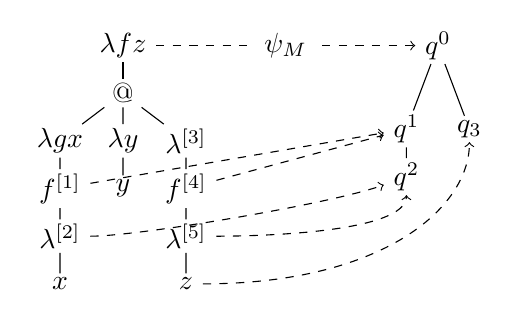
\begin{tikzpicture}[baseline=(root.base),level distance=4ex,sibling distance=8mm,inner ysep=0.5mm]
\path
node (root){$\lambda f z$}
child{node{$@$}
 child{node{$\lambda g x$} child{node(f1){$f^{[1]}$}child{node(l2){$\lambda^{[2]}$}child{node{$x$}}}}}
 child{node{$\lambda y$} child{node{$y$}}}
 child{node{$\lambda^{[3]}$} child{node(f4){$f^{[4]}$} child{node(l5){$\lambda^{[5]}$}child{node(z){$z$}}}}}
}
+(4cm,0)
node (q0){$q^0$}
child[level distance=7ex]{node(q1){$q^1$} child[level distance=4ex]{node(q2){$q^2$}}}
child[level distance=7ex]{node(q3){$q_3$}};
\draw[dashed,->] (root) -- node[fill=white]{$\psi_M$} (q0);
\draw[dashed,->] (f1) -- (q1);
\draw[dashed,->] (f4) --  (q1);
\draw[dashed,->] (l2) .. controls +(0:1cm) and +(200:1cm) .. (q2);
\draw[dashed,->] (l5) .. controls +(0:1cm) and +(-90:20pt) .. (q2);
\draw[dashed,->] (z) .. controls +(0:2.5cm) and +(-90:1cm) ..  (q3);
\end{tikzpicture}
\end{minipage}
&
\begin{minipage}{8cm}
\begin{asparablank}
  \item  \Pstr[1cm]{
t = (n){\lambda f z} \cdot
(n2){@} \cdot
(n3-n2,60){\lambda g x} \cdot
(n4-n,45){f^{[1]}}\cdot
(n5-n4,45){\lambda^{[2]}} \cdot
(n6-n3,45){x} \cdot
(n7-n2,35){\lambda^{[3]}} \cdot
(n8-n,35){f^{[4]}} \cdot
(n9-n8,45){\lambda^{[5]}} \cdot
(n10-n,35){z}
}

\item \Pstr[1.2cm]{
t\filter r = (n){\lambda f z} \cdot (n4-n,50){f}^{[1]} \cdot
(n5-n4,60){\lambda}^{[2]} \cdot (n8-n,45){f}^{[4]} \cdot
(n9-n8,60){\lambda}^{[5]} \cdot (n10-n,40){z}}
\item
\Pstr[1.2cm]{ {\varphi_M(t\filter r) =\ } (n){q^0}\cdot
(n4-n,60){q^1}\cdot (n5-n4,60){q^2}\cdot (n8-n,45){q^1}\cdot
(n9-n8,60){q^2}\cdot (n10-n,38){q^3} \in \sem{M}\ .}
\end{asparablank}
\end{minipage}
\end{tabular}
\end{example}



\section{Application of the theory of traversals}

\todo{Ong's work on MSO decidability of infinite trees generated by HORS.}

\todo{Automata characterization of recursion scheme: CPDA = HORS, analyzing the effect of safety constraints on the game model (safe lambda calculus), Colin Stirling's proof of decidability of higher-order matching.}


\section{Related works}

\todo{Pointer Abstract Machine, Krivine Abstract Machine (Danos), head linear reduction.}

\section{Conclusion}

The traversal theory gives us a way to compute beta-reduction locally without having to perform any kind of global substitution.
In effect, what the traversal theory does is to reduce the term using the \emph{head linear reduction strategy}\todo{reference}.
Although the idea of evaluating a term using this strategy is not new, we believe that our presentation presents several advantages and novelties.
Firstly, the Correspondence theorem establishes a clear correspondence with game semantics, namely that traversals gives you a way to compute precisely the revealed game denotation of a term. To our knowledge, although the notion of revealed game semantics was mentioned in previous works (\cite{willgreenlandthesis}), it was never formally defined.
Secondly, the traversal theory reveals the algorithmic aspect of game semantics in the sense that the definition of the traversal rules lends itself very well to automaton characterization. This was testified in \cite{hmos-lics08}, where an automata characterization of Higher-order recursion schemes was established using this theory.
\smallskip

Another advantage of the traversal theory is its efficiency for effectively computing the game semantic denotations of a term.
The traditional approach is to proceed bottom-up by appealing to compositionality.
Although the compositional nature of game semantics is very attractive from a theoretical point of view, in practice it is not efficient to compute a denotation in that way. Indeed, for every subterm one has to compute all the possible ways to interact with the environment for that subterm. But this denotation is then immediately composed with another subterm, which determines part of the environment's behaviour, thus it was wasteful in the first place to consider all the possible environment's behaviour for the first term.

The traversal theory follows a top-down approach which means that we only consider possible behaviour of the outermost environment.
Moreover contrary to the compositional method, there is no need to implement any composition mechanism: the set of traversals is just obtained by following the traversal rules; hiding of internal nodes is postponed until the end.

The lazy nature of the traversal evaluation provides a further source of efficiency: the beta-redexes are computed ``on-demand'' instead of performing a global substitution.
\smallskip

Last but not least, we believe that the syntactic correspondence between game semantics and its syntax
is of pedagogical interest. Game semantics is often found hard to understand due to some obscure technical definitions.
A concrete presentation such as the one given by the traversal theory, allows one to explain game-semantic concepts
(such as P-view, innocence, visibility) from a programmer point of view.


\section{Further works}

\subsection{Verification} As mentioned before, the theory of traversals was first applied to the domain of verification of infinite structures by Ong.
 \todo{Application to the reachability problem.}


\subsection{Automata theory} The traversal theory was also used in \cite{hmos-lics08} to establish an equi-expressivity result between a certain type of automaton device called Collapsible Pushdown Automaton (CPDA) and higher-order recursion schemes (HORS).
One direction of this proof relies on the traversal theory: for a given HORS, a CPDA is constructed that computes precisely the set of traversals over the computation tree of the HORS.
A crucial point which makes this encoding possible is that the structures generated by these devices are of ground type. Such structures cannot interact with their environment which makes their game-semantic denotation very simple: more precisely, the O-view of the traversal does not play any role in the traversal rules and therefore the automaton does not need to keep track of it. A natural question to ask is whether it is possible to find similar automata-characterization for infinite structures of a higher-order.

\subsection{Further correspondences}
The traversal theory that we have presented here captures the lambda calculus fragment of the game model of call-by-name programming languages such as PCF and Idealized Algol. A natural way to extend this work would be to define the appropriate notion of traversal
corresponding to the call-by-value games \cite{plotkin-75, abramsky98callbyvalue}.
